%\documentclass[b5paper,twoside,10pt,sabonnumbers]{RJWThesis}
\documentclass[a4paper,oneside,12pt,sabonnumbers]{RJWThesis}

\usepackage{amsthm}
\usepackage[plain,chapter]{algorithm}
\usepackage{algorithmic}

\includeonly{fractals/fractals}

%% Use scalable, PostScript Type 1 versions of the Computer Modern fonts.
\usepackage{type1cm}

%% Replace the standard Computer Modern Typewriter font LaTeX uses
%% for monospace text with the PostScript font Adobe Courier.
\usepackage{courier}

% To print crop marks
%\usepackage[a4,cam,center]{crop}
%\crop[font=\upshape\mdseries\small\textsf]

\bibliographystyle{abbrv}

\usepackage[pdfborder=0 0 0,draft=false]{hyperref}
\usepackage{graphicx}
\usepackage{pslatex}
\usepackage{sabon}
\usepackage{stmaryrd}
\usepackage{amsmath}
\usepackage{amssymb}
\usepackage{url}

% Global macros used throughout thesis

\newtheorem{thm}{Theorem}
\newtheorem{cor}{Corollary}
\newtheorem{alg}{Algorithm}
\newenvironment{proof}[1][Proof]{\begin{trivlist}
\item[\hskip \labelsep {\bfseries #1}]}{\qed\end{trivlist}}
\newcommand{\magof}[1]{\left\Vert #1 \right\Vert}
\newcommand{\sinc}{\mathrm{sinc}}
\newcommand{\cperp}{c_\perp}
\newcommand{\cpar}{c_\parallel}
\newcommand{\rinterp}{\mathrm{rinterp}}
\newcommand{\linterp}{\mathrm{linterp}}
\newcommand{\qinterp}{\mathrm{qinterp}}
\newcommand{\interp}{\mathrm{interp}}
\newcommand{\slerp}{\mathrm{slerp}}
\newcommand{\qed}{\hfill$\boxempty$}
\newcommand{\libcga}{{\tt libcga}}
\newcommand{\libcgadraw}{{\tt libcgadraw}}

\newcommand{\hugewedge}{\bigwedge}

\renewcommand{\rmdefault}{psb}
\renewcommand{\ttdefault}{pcr}


\begin{document}

\begin{frontmatter}
\renewcommand{\baselinestretch}{1.2}\selectfont
\title{Computer Graphics using Conformal Geometric Algebra}
\subtitle{A dissertation submitted to the\\{\sc University of 
    Cambridge}\\for the degree of\\{\sc Doctor of Philosophy}}
\author{Richard James Wareham\thanks{Robinson College}}
\group{Signal Processing Group}
\department{Department of Engineering}
\maketitle
\cleardoublepage

% Front matter
\vspace*{0.2\textheight}
\noindent Copyright \copyright \number\year\ Richard James Wareham.
\vspace*{1em}\\
\noindent Draft version.\\
\noindent Approximate word count: \input{wordcount.txt}.
\vfill
\noindent Typeset using the \LaTeX{} document preparation system
in the Sabon, Georgia and Computer Modern fonts.
\vfill
\noindent {\sc Signal Processing Group,}\newline
Department of Engineering,\newline
University of Cambridge,\newline
Trumpington Street,\newline
Cambridge, CB2 1PZ, U.K.
\cleardoublepage

\dedication{Dedication}

\tableofcontents
\end{frontmatter}

\begin{mainmatter}
\renewcommand{\baselinestretch}{1.75}\selectfont
\begin{savequote}
\quoteperson{You know we all became mathematicians for the same reason: 
  we were lazy.}{Max Rosenlicht}
\end{savequote}

\chapter{Introduction}
\label{chap:introduction}

It is generally accepted that a four-dimensional projective description of
three-dimensional Euclidean geometry can have various advantages, particularly
when intersections of planes and lines are required. Such projective
descriptions are used extensively in computer vision and graphics where
rotations and translations are usually described by a single $4\times 4$
matrix. Since its inception in the mid-1970s, computer graphics (CG) has
almost universally used linear vector algebra as its mathematical framework.
This is due primarily to two factors; most early practitioners of computer
graphics were mathematicians familiar with it and linear algebra provided a
compact, efficient way of representing points, transformations, lines, etc.

In the early-1980s CG moved out of the realm of Computer Science research and
started to be used in the broader scientific community as an important
research tool both for simulation and visualisation.  Computer Graphics was
then, and to an extent still is, tied to classical vector algebra which has
started to show a number of problems when applied to the problems being
investigated. Amongst these problems were poor generalisation to spaces other
than $\mathbb{R}^3$, great conceptual difficulty in extending problems to
non-Euclidean geometries and manipulating geometric objects other than simple
lines, planes and points.

As computing power becomes cheaper, the opportunity arises to investigate new
frameworks for CG which, although perhaps not providing the time and space
efficiency of vector algebra, may provide a conceptually simpler system or one
of greater analytical power. This thesis investigates the suitability of
Geometric Algebra (GA) as one such approach. As one might hope the original
four-dimensional description of projective geometry fits very nicely into the
Geometric Algebra framework\cite{HZ91,IJPR00}. 

\section{A Brief Overview of Geometric Algebra}

As stated above, classical vector algebra has a number of problems once one
moves away from three-dimensional Euclidean space. Perhaps the clearest
example is the cross-product of two vectors; the product, $\mathbf{a} \times
\mathbf{b}$, is conventionally defined as a vector normal to the plane
containing $\mathbf{a}$ and $\mathbf{b}$ and has magnitude $ab\sin\theta$
where $\theta$ is the angle between $\mathbf{a}$ and $\mathbf{b}$. However the
normal to the plane is only uniquely defined in three-dimensions and has no
meaning in 2- or 1-dimensional space; the cross-product does not generalise to
higher-dimension spaces. The product is an important element of vector algebra
and one can see that performing geometric operations in higher-spaces without
it quickly becomes complex.

\subsection{The products}

It was in an attempt\cite{GA:grassmann} to create an algebra of vectors which
did generalise to higher spaces that a German schoolteacher named Hermann
Gra{\ss}mann (1809--1877) created an \emph{exterior} or \emph{outer} product
of two vectors denoted as $a \wedge b$. For the remainder of this thesis we
have dropped the usual convention of emboldening vectors since in GA they lie
in the same algebra as scalars and do not need to be differentiated; the
nature of the element is either stated explicitly or clear from context.

Gra{\ss}mann's outer product is usually visualised geometrically as the
movement of one vector along the other to form a `directed area'. This is a
new object, neither a vector nor a scalar. It is termed a \emph{bivector}.
Similarly one may form the outer product of this bivector with another vector
to form a directed volume, a \emph{trivector}, or generally a $n$-volume
termed an $n$-vector. 

To differentiate between scalars, vectors, bivectors, etc we say that a scalar
is grade 0, a vector is grade 1, a bivector (formed from two vectors) is grade
2, etc. A $n$-vector has grade $n$.

\begin{figure}
\centering
\includegraphics{geometric}
\caption{Illustration of bi- and trivectors\label{fig:geometric}}
\end{figure}

The usual geometric visualisation is illustrated in figure \ref{fig:geometric}.
It is worth noting that other visualisations may be more appropriate for a specific
application so the reader should not assume a bivector can \emph{only} represent a
directed area. 

A key feature of GA is that the outer-product is anti-commutative and
associative giving
\begin{displaymath}
a \wedge b = - ( b \wedge a)\quad\mbox{and}\quad
a \wedge (b \wedge c) = (a \wedge b) \wedge c = a \wedge b \wedge c.
\end{displaymath}

Most of Gra{\ss}mann's work was largely ignored by the mathematical community.
It was not until William Clifford (1845--1879) investigated Gra{\ss}mann's
algebra in 1878\cite{GA:clifford} that the crucial step which made GA a useful
algebra was made. Unfortunately Clifford's work was, in its turn, also
somewhat ignored in favour of the work done by Hamilton on quaterions and
the development of linear and vector algebra.

Clifford unified Gra{\ss}mann's outer product and the familiar dot
or inner-product into one \emph{geometric product} such that
\begin{displaymath}
ab = a\cdot b + a \wedge b.
\end{displaymath}
An algebra with this product is usually termed a \emph{Clifford algebra}. We
shall use the term Geometric Algebra to mean the \emph{coupling} of Clifford
algebras with an accompanying geometric interpretation.

A second glance at the geometric product shows an interesting feature which
should be noted. In the expression above we are adding a scalar ($a \cdot b$)
to a bivector ($a \wedge b$). That is we are adding a grade 0 element to a
grade 2 element. This combination of differing grade objects is analogous to
complex numbers where we linearly combine a real and imaginary number to form
a complex number. In this case we refer to such a combination of objects of
varying grade as a \emph{multivector}.  As noted earlier we shall refer to all
single-grade elements with lower-case letters but use upper-case letters to
refer to multivectors. The geometric product also gives us a convenient new
definition of the outer and inner products for vectors as
\[
a \wedge b = \frac{1}{2}(ab - ba)\;\mbox{and}
\]
\[
a \cdot b = \frac{1}{2}(ab + ba).
\]

The power of this approach may be illustrated through its application to
rotation. In two dimensions this is easily performed using complex numbers;
representing the vector $[x\ y]$ as the complex number $z = x + iy$, rotation
by $\theta$ radians can be performed by multiplication with $e^{i\theta}$.
William Hamilton (1805--1865) worked for many years to extend this approach to
three-dimensions. He eventually created \emph{quaternions}
\cite{hamilton2,hamilton1}, an algebra with 4 basis elements $\left\{1,
\mathbf{i}, \mathbf{j}, \mathbf{k}\right\}$ from which all elements are
generated through linear combination. This algebra, although functional,
lacked an obvious geometrical interpretation and again didn't generalise
easily to higher-dimensions. We shall visit quaternions later and show how they relate to GA.

\subsection{Rotation via Rotors}

To demonstrate Clifford's approach, consider any three orthonormal basis
vectors of $\mathbb{R}^3$, $\left\{e_1, e_2, e_3\right\}$. We can form
3 different bivectors from these vectors:
\begin{displaymath}
B_1 = e_2e_3,\quad B_2 = e_3e_1,\quad B_3 = e_1e_2.
\end{displaymath}

Note that these are indeed bivectors since the basis vectors are orthogonal and
\[
e_ie_j = e_i \cdot e_j + e_i \wedge e_j = e_i \wedge e_j \quad \mbox{iff} \quad i \ne j
\]

Now consider the effect of $B_3$ on the vectors $e_1$ and $e_1 + e_2$:
\begin{displaymath}
e_1B_3 = e_1^2e_2=e_2 
\end{displaymath}
\begin{displaymath}
(e_1 + e_2)B_3 = e_1B_3 + e_2B_3 = e_2 + e_2e_1e_2 = e_2 - e_1e_2^2 = e_2 - e_1
\end{displaymath}

\begin{figure}
\centering
\includegraphics{rotation}
\caption{The rotation effect of bivector $B_3 = e_1e_2$\label{fig:rotation}}
\end{figure}

From figure \ref{fig:rotation} it is clear that $B_3$ has the effect
of rotating the vectors counter-clockwise by 90 degrees. It is, in fact, a
general property that the bivector $e_ie_j$ will rotate a vector 90 degrees in
the plane defined by $e_i$ and $e_j$. At first glance this seems to offer
little more than quaternions, but at no point have we assumed that we are
working in three-dimensional space; this method also works in higher-dimension
spaces.

We can also easily extend to general rotations; it is trivial to
show that $B_3$ squares to $-1$:
\begin{displaymath}
B_3^2 = e_1e_2e_1e_2 = -e_1e_2e_2e_1 = -1
\end{displaymath}

We can represent any vector $x$ in the plane defined by $e_1$ and
$e_2$ using
\begin{eqnarray*}
x & = & r ( e_1 \cos \theta + e_2 \sin \theta) \\
  & = & e_1 r ( \cos \theta + B_3 \sin \theta)
\end{eqnarray*}
where $r$ is the distance of the point $x$ from the origin (i.e.\ $r = \sqrt{x^2}$)
and $\theta$ is the angle $x$ makes with $e_1$. 
By taking the Taylor expansion of cosine
and sine and re-arranging the coefficients it can be shown that
\[
e^{B_3\theta} = \cos \theta + B_3 \sin \theta
\]
which is the GA analogue of de Moivre's theorem for complex
numbers.

We can thus represent any vector $x$ which lies in the plane of the
bivector $B_3$ by
\[
x=e_1re^{B_3\theta}
\]

From this the same argument used for rotation in the complex plane 
can be used to show that rotation by
$\phi$ radians in the plane of $B_3$ is accomplished by $x \mapsto x'$
where
\begin{displaymath}
x' = xe^{B_3\phi} = x (\cos \phi + B_3 \sin \phi)
\end{displaymath}

This has all taken place in two dimensions for the moment but nothing in our
discussion has assumed this. In fact we can specify a unit bivector $B_3 = ab$ in
three dimensions and rotate vectors in the place defined by $a$ and $b$ using
the expression above.

\begin{figure}
\centering
\includegraphics{rotation2}
\caption{Rotating vectors in arbitrary planes\label{fig:rotation2}}
\end{figure}

Careful consideration must be given to the case where the vector to be
rotated, $x$, does not lie on the plane of rotation as in figure
\ref{fig:rotation2}. Firstly decompose the
vector into a component which lies in the plane $x_\parallel$ and one
normal to the plane $x_\perp$
\[
x = x_\parallel + x_\perp
\]

Now consider the effect of the following
\begin{eqnarray*}
e^{-B_3\phi/2}
x
e^{B_3\phi/2}
& = & \left(\cos \frac{\phi}{2} - B_3 \sin \frac{\phi}{2}\right)
(x_\parallel + x_\perp )
\left(\cos \frac{\phi}{2} + B_3 \sin \frac{\phi}{2}\right) \\
& = & x_\parallel (\cos \phi + B_3 \sin \phi) + x_\perp
\end{eqnarray*}
since bivectors anti-commute with vectors in their plane (e.g. 
$e_1(e_2e_1) = -e_2 = -(e_2e_1)e_1$) and commute with
vectors normal to the plane (e.g.\ $e_1(e_2e_3) = (e_2e_3)e_1$).
We have thus succeeded in rotating the component of the vector 
which lies in the plane without affecting the component normal
to the plane --- we have rotated the vector around an axis normal to
the plane.

This leads to a general method of rotation in any plane; we
form a bivector of the form $R = \exp({-B\phi/2})$ for a given rotation 
$\phi$ in a plane specified by the unit bivector $B$. The transformation
is therefore performed by
\begin{displaymath}
x \mapsto RxR^{-1}.
\end{displaymath}
We refer to these bivectors which have a rotational effect as \emph{rotors}.
Figure \ref{fig:rotation2} shows the various objects used. Later we shall
extend the term \emph{rotor} to refer to an element of the algebra which
performs some well defined transformation.

Computing $R^{-1}$ is rather difficult analytically and can sometimes
require a full $2^n$-dimension matrix inversion for a space of
dimension $n$. To combat this we define
the \emph{reversion} of a $n$-vector $X = e_ie_j...e_k$ as
\[
\tilde{X} = e_k...e_je_i
\]
i.e. the literal reversion of the components. By looking at the expression for
$R$ it is clear that $\tilde{R} \equiv R^{-1}$ for rotors. Computing
$\tilde{R}$ is easier since it generally just involves changing the sign of
components when an element is resolved onto a set of basis elements.

Note that in spaces with dimension $n$, the maximum grade object possible is
an $n$-grade one. We denote the $n$-vector $e_1 \wedge ... \wedge e_n = I$ as
the \emph{pseudoscalar} and the product $xI$ as the \emph{dual} of a vector or
$x^*$. The dual is similarly defined for general multivectors. The
pseudoscalar is so termed because it commutes with all elements of the
algebra.

\subsection{Relation to quaternions}
\label{sec:quaternions}

It is worth comparing this method of rotation to rotation via
quaternions. The three bivectors $B_1,B_2$ and $B_3$ act identically to the
three `imaginary' components of quaternions, $\mathbf{i}, -\mathbf{j}$ and
$\mathbf{k}$ respectively. The sign difference between $B_2$ and $\mathbf{j}$
is due to the fact that the quaternions are not derived from the usual
right-handed orthogonal co-ordinate system. This handedness mismatch often
leads to annoying sign errors in quaternion-based algorithms.

Using quaternions, a particular rotation is represented via the unit quaternion 
$q$ given by
\[
q = q_0 + q_1 \mathbf{i} + q_2 \mathbf{j} + q_3 \mathbf{k}
\]
where $q_0^2 + q_1^2 + q_2^2 + q_3^2 = 1$. 
It is known\cite{ACM:325242} that quaternions are particularly useful
not only for representing rotations but also for interpolating them.
This interpolation is performed by considering the unit quaternion to
be a point on a four-dimensional hyper-sphere and interpolating over 
the surface of this sphere. For example, given a pair of rotations specified
by the
unit quaternions $q_0$ and $q_1$, the \emph{spherical linear interpolation} (SLERP)
would be
\[
q = \left\{
\begin{array}{ll}
q_0(q_0^{-1}q_1)^\lambda & {\rm ~if~} q_0 \cdot q_1 \ge 0 \\
q_0(q_0^{-1}(-q_1))^\lambda & {\rm ~otherwise}
\end{array}
\right.
\]
where $\lambda$ varies in the range $(0,1)$ \cite{slerp}.

Recall that the locus of $\exp(i\theta)$ is the unit
circle. It is straightforward to show that, for some normalised
bivector $B$, the locus of the action of $\exp(B\theta)$ upon a point with respect to varying
$\theta$ is also a circle in the plane of $B$. Hence, if we consider
some rotations $R_1, R_2 = \exp(B)R_1$, where 
$B$ is some normalised bivector, it is clear that
the quaternionic interpolation is exactly given by
\[
R_\lambda = (R_2 \tilde{R}_1)^\lambda R_1 = \exp(\lambda B) R_1
\]
where $\lambda$, the interpolation parameter, varies in the range $(0,1)$. A
further moment's thought will reveal that this method is not confined to three
dimensions, like quaternionic interpolation, but instead readily generalises
to higher-dimensions. It is also worth noting the extreme similarity between the
rotor interpolation and the quaternionic interpolation. In fact pure-rotation
rotors behave identically to quaternions and we shall see later how this SLERP
interpolation scheme may be extended to include translation as well as rotation.

\subsection{The Conformal Model of Geometric Algebra}

In the Conformal Model\cite{hestenes} we extend the space by adding two
additional basis vectors. The notation we use will follow the original
notation given in \cite{HS84}. Let $x$ be a vector in a space denoted
${\cala}(p,q)$.  The annotation $(p,q)$ shall be termed the \emph{signature}
of the space.  A given signature, $(p,q)$, implies that we may construct an
orthogonal basis for the space, $\{e_i\}$, $i=1,\cdots,n=p+q$ where $e_i^2=+1$
for $i=1,\cdots,p$ and $e_i^2=-1$ for $i=p+1,\cdots,n$; i.e.\ we take a
general mixed signature space.  

To perform geometric operations using GA we now extend the space 
to ${\cala}(p+1,q+1)$ via the inclusion of two additional orthogonal
basis  vectors, $e$ and
$\bar{e}$, such that
%
\[  e^2=+1,\;\;\;\; \bar{e}^2= -1
\]
%

Note that if $x \in {\cala}(p,q)$, then $e\cdot x =
\bar{e}\cdot x = 0$ since $e_i\cdot e=e_i \cdot \bar{e} = 0$
for $i=1,\cdots,n$. We now define vectors $n$ and
$\bar{n}$ as
%
\[ n = e + \bar{e}  \qquad  \bar{n} = e - \bar{e}.
\label{nequations}
\]
These vectors will be useful later. It is easy to see that
$n$ and $\bar{n}$ are \emph{null} vectors since
%
\begin{eqnarray}
n^2  & = & (e + \bar{e})\cdot(e + \bar{e}) = e^2 + 2e\cdot\bar{e} + \bar{e}^2 \nn \\
       & = &  1 + 0 - 1 = 0  \nn
\end{eqnarray}
and
\begin{eqnarray}
\bar{n}^2  & = & (e - \bar{e})\cdot(e - \bar{e}) = e^2 - 2e\cdot\bar{e} + \bar{e}^2 \nn \\
       & = &  1 - 0 - 1 = 0.     \nn
\end{eqnarray}
%
We also note a number of useful identities for $n$, $\bar{n}$ and $x \in \cala(p,q)$:
%
\begin{eqnarray}
n\cdot\bar{n} & = & (e + \bar{e})\cdot(e - \bar{e}) = e^2 - \bar{e}^2 = 2 \nn \\
x\cdot n = x\cdot \bar{n} & = & 0. \nn 
\end{eqnarray}
%
It is equally easy to show that if we define the bivector $E = n \wedge \bar{n}$ 
then $E^2 = 4$
%
\begin{eqnarray}
  E^2 & = &  (n\wedge \bar{n})\cdot(n\wedge \bar{n}) \nn \\
  & = &  (n\cdot\bar{n})(n\cdot\bar{n}) - n^2 \bar{n}^2 \nn \\
  & = &  4
  \end{eqnarray}
  %
since $n\cdot\bar{n}=2$ and $n^2=\bar{n}^2=0$.

In the conformal model we use general null-vectors to represent points and 
build up objects.
In $\cala(p,q)$ we map a point $x \in \cala(p,q)$ to a vector
$F(x) \in \cala(p+1,q+1)$. Using this representation we find that 
complex geometric operations may be performed
by simple algebraic manipulation of $F(x)$. The specific mapping
used is the Hestenes (\cite{HS84}, page 302) representation
%
\begin{equation}
F(x)=-\frac{1}{2}(x-e)n(x-e)
\end{equation}
%
where, substituting for $n=e+\bar{e}$ and using the fact that
$\bar{e}\cdot x = 0 = \bar{e}\cdot e = n\cdot x$, it is possible
to rewrite this equation in terms of the null
vectors as follows
%
\begin{equation}
  F(x) = \frac{1}{2}(x^2n + 2x - \bar{n})
\end{equation}
%
which is similar to the form which is used in the more recent
`horosphere' formulations of the conformal framework
\cite{oldwine}. We will see that there is some choice as
to what factor we put in front of the $x^2n + 2x -
\bar{n}$ expression; we choose $\half$ so that our
normalisation condition for null vectors, which allows us to
compute the reverse mapping $F(x) \mapsto x$ independent of the
absolute scale of $F(x)$, becomes
%
\[ F(x)\cdot n = -1.  \]
%

We will see that it will often be necessary to work with
normalised `unit' lines, planes, circles and spheres in order to
apply the various formul\ae\ which will be so
important in later sections. It is also worth noting that the
mapping as it stands above is dimensionally inconsistent. In following
chapters it will be shown how compensating for this inconsistency 
can allow one to extend the approach to various non-Euclidean geometries.

It is possible to show that $F(x)$ is always a null vector for
any $x$ by directly evaluating $[F(x)]^2$
%
\begin{eqnarray}
 [F(x)]^2 & = &  \frac{1}{4}(x^2n + 2x - \bar{n})\cdot (x^2n + 2x - \bar{n}) \nn \\
              & = & -\frac{1}{2}x^2 n\cdot \bar{n} + x^2  \nn \\
              & = &  -x^2 + x^2 = 0
\end{eqnarray}
%

We have mapped vectors in ${\cala}(p,q)$ into \emph{null}
vectors in ${\cala}(p+1,q+1)$ and this is precisely the horosphere 
construction. It also shows the need to impose a normalisation
constraint upon the resultant null vectors as they remain null 
irrespective of absolute scale.
More generally we can show that all null vectors in $\cala(p+1,q+1)$
must be the result of mapping some vector $x \in \cala(p,q)$ as above;
any vector $X \in {\cala}(p+1,q+1)$ can be written as
%
\[ X = an + bx + c\bar{n}  \]
%
where $x = x^ie_i$, $i=1,\cdots,p+q$ and hence $x \in \cala(p,q)$.
We can say that $X\cdot n = 2c$ and $X\cdot \bar{n}=2a$ (since $n$ is 
null and $x\cdot n = 0$). Therefore $a$
and $c$ are uniquely determined. However we can also write our
general $X$ as  $X=b{x}^ie_i + \alpha e + \bar{\alpha}\bar{e}$ for 
suitable scalars $\alpha$ and $\bar{\alpha}$ and
have $X\cdot e_j= bx^j$ ($j=1,\cdots,p+q$). So, whilst the product
$bx^j$ is uniquely defined by $X$, $b$ and $x^j$ individually are
not. Now suppose that $X$ is null so that $X^2=0$
%
\begin{eqnarray}
X^2 & = &   (an + bx + c\bar{n})\cdot (an + bx + c\bar{n}) \nn \\
       & = &  2ac n\cdot \bar{n} + b^2x^2 \nn \\
       & = & b^2x^2 + 4ac = 0
       \label{condition}
\end{eqnarray}
%

From this we are easily able to see that any null vector can be
written in the form
%
\begin{equation}
\lambda (x^2n + 2x - \bar{n}) \label{null}
\end{equation} 
%
since if $(an + bx + c\bar{n}) = \lambda(x^2n + 2x -
\bar{n})$ we have that
%
\[c=-\lambda\;\;\;\; \lambda x^2 = a \;\;\;\mbox{and}\;\;\; 2\lambda = b\]
%
and we can then eliminate $\lambda$ from these last two
equations to give the condition $b^2 x^2 = -4ac$. This
is precisely the condition given in
equation~\ref{condition}.

These results may now be used to provide a projective mapping
between ${\cala}(p,q)$ and  ${\cala}(p+1,q+1)$. Specifically that the
family of null vectors $\lambda(x^2n + 2x - \bar{n})$,
in ${\cala}(p+1,q+1)$ are taken to correspond to the
single point $x\in {\cala}(p,q)$. If $x$ is the origin
then we see that $F(x) = -\frac{1}{2}\bar{n}$ and we may therefore associate
null vectors parallel to $\bar{n}$ with the origin. 
We will see later that when we \emph{invert} $\bar{n}$ 
we obtain $n$, suggesting
that we associate null vectors parallel to $n$ with the 
\emph{point at infinity} (the usual result of inverting the origin).

When we look at the inner product of normalised null vectors in
${\cala}(p+1,q+1)$ we discover something very
interesting. If $A$ and $B$ in ${\cala}(p+1,q+1)$
represent the points $a$ and $b$ in ${\cala}(p,q)$, then
%
\begin{eqnarray} A\cdot B &  =  &  F(a)\cdot F(b) \nn \\
            &  =  &  \frac{1}{4}(a^2n + 2a - \bar{n})\cdot (b^2n + 2b -
            \bar{n})\nn \\
            & = &    -\frac{1}{2}a^2 + a\cdot b - \frac{1}{2}b^2 \nn \\
            &  =  &  -\frac{1}{2}(a-b)^2
\end{eqnarray}
%
and we see that $A\cdot B$ is related to the Euclidean
distance between points $a$ and $b$. 
We can therefore define the Euclidean distance between two
point representations as
\begin{equation}
d(A,B) = \sqrt{-2 (A \cdot B) }
            \label{distance}
\end{equation}
This property of the
conformal space and its relationship to \emph{distance geometry}
\cite{distgeom} is discussed at more length in \cite{oldwine}. 
The mapping and properties described here were outlined
originally in \cite{HS84}.

\subsubsection{Rotations}

In usual descriptions of GA (without the use of the conformal model)
rotations are performed with elements of the algebra termed
\emph{rotors}. In this section we aim to show that these rotors may be used
unchanged on the null vectors representing points.
Let $x \mapsto Rx\tilde{R}$ with $x\in {\cala}(p,q)$ and $R$ be a
rotor in the Geometric Algebra over ${\cala}(p,q)$. Consider
what happens when $R$ acts upon $F(x)$; i.e.\ the nature of
$RF(x)\tilde{R}$
%
\[ RF(x)\tilde{R} =\frac{1}{2} R(x^2n + 2x - \bar{n})\tilde{R} =\frac{1}{2}[ x^2Rn\tilde{R}
+ 2Rx\tilde{R} - R\bar{n}\tilde{R}] \].
%
Since $R$ is a rotor it contains only even blades and therefore 
commutes with
$n$ and $\bar{n}$  
%($e_in=-ne_i$, so if we have an even number of $e_i$s we
%		have commutation), so that $Rn\tilde{R} = R\tilde{R} n = n$ and
%$R\bar{n}\tilde{R} = \bar{n}$. Thus we have
so
%
\begin{equation} RF(x)\tilde{R} = \frac{1}{2}(\hat{x}^2n + 2\hat{x} - \bar{n})
	\end{equation}
%
where $\hat{x}=R x \tilde{R}$. We have therefore shown that rotors in
${\cala}(p,q)$ remain rotors in ${\cala}(p+1,q+1)$ in that they retain
their action about the point $x$ represented by $F(x)$. To summarise
%
\begin{equation} x \mapsto Rx\tilde{R} \qquad \Leftrightarrow \qquad F(x) \mapsto
F(Rx\tilde{R}) \end{equation}
%

\subsubsection{Translators}

Translation along a vector $a$ is defined for our purposes as the
mapping $x\mapsto x+a$ for some $x,\,a \in \cala(p,q)$.
In this
section we will show that this is performed by applying a 
rotor $R=T_a = \exp\left({\frac{na}{2}}\right)$ to $F(x)$.

Before proceeding with the proof we should note that in some non-Euclidean
geometries the addition operator, when viewed as a translation operator, is
non-commutative; translation of geodesic $A$ along geodesic $B$ is not the
same, in general, as translation of $B$ along $A$. For the moment we shall
ignore this but it will become important again in later chapters on 
non-Euclidean geometries.

Returning to the form of the translation rotor, consider the usual power series 
expansion of the exponential which we may immediately simplify to
%
\begin{equation}
R=T_a = \exp\left({\frac{na}{2}}\right) = 1 + \frac{na}{2} +
\frac{1}{2}\left(\frac{na}{2}\right)^2 + \cdots   = 1 +
\frac{na}{2}
\end{equation}
%
since $n$ is null, $an = -na$ and therefore the higher order terms are all
zero. We now see how $R$ acts on the vectors $n$, $\bar{n}$ and $x$.
%
\begin{eqnarray}
 Rn\tilde{R} & = & \left(1 + \frac{na}{2}\right)n\left(1 + \frac{an}{2}\right) \nn \\
                & = &  n + \frac{1}{2}nan + \frac{1}{2}nan + \frac{1}{4}nanan \nn \\
                & = & n
                \label{rntrans}
\end{eqnarray}
%
again using  $an= - na$ and $n^2=0$.    Similarly we can
show that
%
\begin{eqnarray}
 R\bar{n}\tilde{R} & = &  \bar{n}  - 2a - a^2n \\
 Rx\tilde{R}          & = &  x + n(a\cdot x)
\end{eqnarray}
%
Immediately we see that our interpretation of $n$ being the point at
infinity and $\bar{n}$ being the origin is consistent with our claim that
$R$ represents the translation $x \mapsto x+a$ since 
$R(-\bar{n})\tilde{R} = F(a)$
and the point at infinity is unchanged by finite translation.

We can now also see how the rotor acts on $F(x)$
%
\begin{eqnarray}
RF(x)\tilde{R} & = & \left(1 + \frac{na}{2}\right)\half(x^2n + 2x - \bar{n})\left(1 + \frac{an}{2}\right) \nn \\
                & = &  \half(x^2n + 2(x + n(a\cdot x)) - (\bar{n} - 2a - a^2n))   \nn \\
                & = &  \half((x+a)^2n + 2(x+a) - \bar{n}) \nn \\
                & = &  \half(\hat{x}^2 n + 2\hat{x} - \bar{n}) = F(x+a)
\end{eqnarray}
%
where $\hat{x}=x+a$ and thus translations in
${\cala}(p,q)$ can be performed by the
rotor  $R=T_a$ defined above. To summarise
 %
 \begin{equation}
x \mapsto x+a \qquad \Leftrightarrow \qquad F(x) \mapsto T_a
F(x) \tilde{T}_a = F(x+a)
\end{equation}

\subsubsection{Inversion}

In the usual three-dimensional geometric algebra we can reflect a vector $a$
in a plane with unit normal $n$ by `sandwiching' the vector between the
normal, $-nan$ \cite{IJCV98}. Sandwiching the object \emph{to be reflected}
between the object \emph{in which we wish to reflect} is a very general
prescription in GA and one which will be used heavily in later parts of the
thesis.  In this section we look at how inversions are brought about by this
same reflection operation.

By `inversion' we mean the mapping $x \mapsto \frac{x}{x^2}$ or,
equivalently, for non-singular areas, $x \mapsto x^{-1}$. Firstly, we look 
at the reflection in $e$ of various vectors
%
\[ -ene  = -ee\bar{n} = -\bar{n} \] 
since $ne = (e+\bar{e})e=(e^2+\bar{e}e)= (e^2 - e\bar{e}) = e\bar{n}$. 
Similarly, we can show that a number of reflection properties hold
%
\begin{eqnarray} -ene & = &  -\bar{n}  \\ -e\bar{n}e & = &  -{n}  \\ -exe & = &
x \end{eqnarray}
%
and finally we may observe what happens to $F(x)$ under reflection in $e$
%
\begin{eqnarray} -eF(x)e & = &  -e\half(x^2n + 2x - \bar{n})e  \nn \\ & = &
\half\left[-x^2\bar{n} + 2x + n\right] \nn \\ & = &  x^2\half\left[
\frac{1}{x^2}n + 2\frac{x}{x^2} - \bar{n}\right] \nn \\ & = &  x^2
F\left(\frac{x}{x^2}\right) \end{eqnarray}
%

We have, therefore, shown that the inversion operation in ${\cala}(p,q)$ can be
performed via the reflection in $e$ of the representation in ${\cala}(p,+1q+1)$.
 %
 \begin{equation} x \mapsto \frac{x}{x^2} \qquad \Leftrightarrow \qquad F(x) \mapsto
 -\frac{eF(x)e}{x^2} = F\left(\frac{x}{x^2}\right) \end{equation}
%

Since the absolute scale of $F(x)$ is irrelevant, as we always rescale to
impose our normalisation constraint, we can omit the scaling by $x^{-2}$.  It
is also irrelevant, by the same logic, whether we take $-e(\cdot)e$ or
$e(\cdot)e$ as the reflection and henceforth we will use $e(\cdot)e$ for
convenience. This `sandwiching' operation will be a common one in the algorithms
we will describe in subsequent chapters.
%We reiterate here that later the concept of
%reflection of a quantity in an object being brought about by this method
%of `sandwiching' will be a very common operation in 
%the
%quantity between the object 
%is crucial to much of our code for fast three-dimensions
%manipulations.

\subsubsection{Dilators}


A dilation by a factor of $\alpha$ is the mapping
$x \mapsto \alpha x$. In this section we investigate how
to form a rotor which has the action of dilating about the
origin. We start by considering the rotor $R = D_{\alpha} =
\exp\left({\frac{\alpha}{2}e\bar{e}}\right)$ and a number of
relations which can easily be verified
%
\begin{eqnarray}
   -e\bar{e}n  = &  {n} & = ne\bar{e}  \nn \\
   -\bar{n}e\bar{e} = &  \bar{n} & =  e\bar{e}\bar{n}  \label{eneqn}
\end{eqnarray}
%
We can now look at what $RF(x)\tilde{R}$ gives
%
\begin{eqnarray}
D_\alpha F(x) \tilde{D}_\alpha & = & \exp\left({\frac{\alpha}{2}e\bar{e}}\right)\half\{ x^2n + 2x - \bar{n}\}\exp\left({-\frac{\alpha}{2}e\bar{e}}\right) \nn \\
   &  =  &  \half(x^2  \exp\left({\alpha e\bar{e}}\right)n + 2x - \exp\left({\alpha e\bar{e}}\right)\bar{n}) \nn \\
   & = &  \half(x^2 \exp\left({-\alpha}\right) n + 2x - \exp\left({\alpha}\right)\bar{n}) \nn \\
   & = & \exp\left({\alpha}\right)\half\left\{\exp\left({-2\alpha}\right)x^2n + 2\exp\left({-\alpha}\right)x - \bar{n}\right\} \nn \\
   & = & \exp\left({\alpha}\right)\half\left\{\hat{x}^2n + 2\hat{x} -\bar{n}\right\}
\label{Deqn}
\end{eqnarray}
%
where $\hat{x} = \exp\left({-\alpha}\right)x$. The above steps can be
verified by considering $\exp\left({-\frac{\alpha}{2}e\bar{e}}\right)$ as
the expansion $1 - \frac{\alpha}{2}e\bar{e} +
\frac{1}{2!}\left(\frac{\alpha}{2}e\bar{e}\right)^2 +
\cdots$ and using the relations given in
equation~\ref{eneqn}.
Again noting that the absolute scale of $F(x)$ doesn't matter we
have therefore shown that dilations  in ${\cala}(p,q)$ can be performed by
the rotor    $R=D_\alpha$
 %
 \begin{equation}
x \mapsto \exp({-\alpha})x \qquad \Leftrightarrow \qquad F(x)
\mapsto  D_{\alpha} F(x) \tilde{D}_{\alpha} =
\exp({\alpha})F(\exp({-\alpha})x)
\end{equation}
%
Note that the signs are incorrect in the equivalent
equations in \cite{HS84}, p.303, equation~3.22. It is worth noting
that dilation about any other point may be achieved by concatenating the
appropriate rotors to move that point to the origin, dilate and move back.


\subsubsection{Special conformal transforms}


We have seen above that we are able to express rotations,
inversions, translations and dilations in ${\cala}(p,q)$
by rotations and reflections in  ${\cala}(p+1,q+1)$. This
now leads us to consider \emph{special conformal
transformations}. These are essentially transformations
which preserve angles and are defined by the motion
%
\begin{equation}
x \mapsto  x \frac{1}{1 + ax}
\end{equation}
%

Some thought reveals this transform to be 
a combination of inversion, translation and inversion again
%
\begin{eqnarray}
x   & \stackrel{\longmapsto}{_{\mbox{inversion}}} & \frac{x}{x^2} \nn \\
     &  \stackrel{\longmapsto}{_{\mbox{translation}}} & \frac{x}{x^2} + a  \equiv \frac{x}{x^2}(1+xa)  \nn \\
     &  \stackrel{\longmapsto}{_{\mbox{inversion}}} & \frac{\frac{x}{x^2} + a}{(\frac{x}{x^2} + a)(\frac{x}{x^2} + a)} \nn \\
   & = & \frac{x+ ax^2}{1+2a\cdot x + a^2x^2} = x\frac{1}{1 + ax}
\end{eqnarray}
%
since $\frac{1}{1+ax} = \frac{1+xa}{(1+ax)(1+xa)}$. The
final line in the above expression shows us that
$x\frac{1}{1 + ax}$ is indeed a vector since $x+ ax^2$ is
a vector. As we have built up the special conformal
transformation via inversions and translations, we know
exactly how to construct the ${\cala}(p+1,q+1)$ operator
that performs such a transformation by simply chaining the
rotors for inversion and translation we derived above.
The required rotor is therefore given by
%
\begin{equation}
 K_a = eT_a e,\qquad {\mbox{so that}} \qquad x\mapsto K_a x \tilde{K}_a
\end{equation}
%
and
\begin{equation}
   K_a x \tilde{K}_a = e\left\{ T_a(exe)\tilde{T}_a\right\}e
\end{equation}
%
%Now recall that $T_a = 1+ \frac{na}{2}$, $a\in
%{\cala}(p,q)$, so that $eT_ae = e\{1+\frac{na}{2}\}e =
%e^2 + \frac{1}{2}enae = 1-\frac{1}{2}\bar{n}a$. Thus, we
Substituting for the rotors above we can write our special conformal rotor as
%
\begin{equation}
K_a = 1 - \frac{1}{2}\bar{n}a
\end{equation}
%
We are now in a position to see what happens when we act
on $F(x)$ with $K_a$
%
\begin{eqnarray}
 K_a F(x) \tilde{K}_a & = & eT_a(eF(x)e)\tilde{T}_a e \nn \\
               & = & eT_a( - x^2 F(\frac{x}{x^2}))\tilde{T}_a e \nn \\
       & = &  -x^2 e\left\{ F(\frac{x}{x^2} +a)\right\} e \nn \\
& = & -x^2\left\{- \left(\frac{x}{x^2} + a\right)^2
F\left(\frac{\left(
\frac{x}{x^2} + a\right)}{\left(\frac{x}{x^2} + a\right)^2}\right)\right\} \nn \\
          & = & (1 + 2a\cdot x + a^2x^2)F\left( x\frac{1}{1+ax}\right)
\end{eqnarray}
%
The end result is therefore
%
\begin{equation}
x\mapsto x\frac{1}{1+ax}  \qquad \Leftrightarrow \qquad  F(x)
\mapsto (1+2a\cdot x + a^2x^2)F\left(x\frac{1}{1+ax}\right)
\end{equation}
%

%
\subsection{Observations}
We can see that, from the above, the following results are true:
%
\begin{eqnarray}
R n \tilde{R} &  =  &   n \;\;\; \mbox{for $R$ a
rotation, since} \;\;\; n\tilde{R}=\tilde{R}n
 \nn \\
 R n \tilde{R} &  =  &   n \;\;\; \mbox{for $R$ a
translation (equation~\ref{rntrans}}) \nn \\
n\tilde{R}=\tilde{R}n \;\;\mbox{and}\;\;\; R n \tilde{R}
& = & \exp{(-\alpha )}n \;\;\;\mbox{for dilations} \nn
\end{eqnarray}
%

Thus rotations, translations and dilations leave $n$, which we identify with
the point at infinity, unchanged up to a scale factor. This is a fact which
will be important to us in subsequent chapters. Indeed, we find that the
underlying geometry described by the rotors is related to the element of the
algebra which the rotors hold invariant. We will see later that the five-dimensional
conformal setup provides a framework in which we can simply describe
non-Euclidean geometries in such terms.

\section{Existing implementations}

%One of the goals of this PhD was to continue to develop a software
As part of the research presented here a library designed to help with the
implementation of CGA-based algorithms in an efficient manner was created.
Before work started on designing the software, several existing systems were
investigated. All of the following packages were designed to provide
high-level access to numerical computations using GA.

\subsection{CLUCalc \& CLUDraw}


CLU \& CLUDraw were written by Christian Perwass and may be obtained from his
web-site\cite{CLU}. Of all the systems, this
is the only one designed both for CGA and the visualisation of spheres,
circles, etc.\ directly from the CGA model.

It is written in C++ and uses the object-oriented features of the language
extensively. Multivectors are represented as objects and operations upon
them are performed by overloading the standard operators of the C++
language. 

CLU is a library designed for numerical computations and is not limited
to the signature used for the conformal model but also has support for
other signatures. CLUDraw is a library designed to take multivectors calculated
by CLU and provide a convenient way to visualise them as spheres, lines, planes,
etc. 

Although it provides a convenient interface, the heavy use of C++ object-orientation
and operator overloading within the library results in a rather high
computational overhead. The decoupling of the calculation engine and
visualisation engine however provides the useful ability to remove the
graphics code in a clean manner.


%\subsection{GABLE}
%
%TBC

\subsection{Gaigen}

The Gaigen 
homepage\cite{Gaigen} describes 
it as
\begin{quote}
Gaigen is a program which can generate implementations of geometric algebras. It generates C++, C and assembly source code which implements a geometric algebra requested by the user. People who are new to geometric algebra may think that there is only one geometric algebra. However, there are many different geometric algebras. The properties that make these algebras different are, among others, their dimensionality and the signature of their basis vectors. Each of these different algebras may be useful for different applications.
\end{quote}
The user can select the signature of the space and generate C-code to implement
it. The code it generates is efficient and compact. The Gaigen2 project has
moved into a different direction; instead of accelerating individual products a
different approach to making an efficient implementation is used with a
different internal representation. Gaigen doesn't possess a visualisation
engine by default.

Gaigen, although fine for general purpose use, wasn't suitable for this
PhD as, ultimately, it was desired that a similar API would be found for
both software and hardware implementations and it was felt that having our
own implementation would lead to greater flexibility in this area.

\begin{table}
\centering
\textbf{Geometric Product Multiplication Table}\\
\rule{0cm}{0.3cm}
%Geometric Product Multiplication Matrix:\\
%\begin{equation}\left[\begin{array}{cccccccc}
%+A_{0} & +A_{1} & +A_{2} & +A_{3} & -A_{12} & -A_{13} & -A_{23} & -A_{123}\\
%+A_{1} & +A_{0} & +A_{12} & +A_{13} & -A_{2} & -A_{3} & -A_{123} & -A_{23}\\
%+A_{2} & -A_{12} & +A_{0} & +A_{23} & +A_{1} & +A_{123} & -A_{3} & +A_{13}\\
%+A_{3} & -A_{13} & -A_{23} & +A_{0} & -A_{123} & +A_{1} & +A_{2} & -A_{12}\\
%+A_{12} & -A_{2} & +A_{1} & +A_{123} & +A_{0} & +A_{23} & -A_{13} & +A_{3}\\
%+A_{13} & -A_{3} & -A_{123} & +A_{1} & -A_{23} & +A_{0} & +A_{12} & -A_{2}\\
%+A_{23} & +A_{123} & -A_{3} & +A_{2} & +A_{13} & -A_{12} & +A_{0} & +A_{1}\\
%+A_{123} & +A_{23} & -A_{13} & +A_{12} & +A_{3} & -A_{2} & +A_{1} & +A_{0}
%\end{array}\right]
%\end{equation}

%Geometric Product Multiplication Table:\\
\begin{tabular}{|r||c|c|c|c|c|c|c|c|}
\hline
 &
1 & $e_{1}$ & $e_{2}$ & $e_{3}$ & $e_{12}$ & $e_{13}$ & $e_{23}$ & $e_{123}$\\
\hline
\hline
1 & +1 & +$e_{1}$ & +$e_{2}$ & +$e_{3}$ & +$e_{12}$ & +$e_{13}$ & +$e_{23}$ & +$e_{123}$\\
\hline
$e_{1}$ & +$e_{1}$ & +1 & +$e_{12}$ & +$e_{13}$ & +$e_{2}$ & +$e_{3}$ & +$e_{123}$ & +$e_{23}$\\
\hline
$e_{2}$ & +$e_{2}$ & -$e_{12}$ & +1 & +$e_{23}$ & -$e_{1}$ & -$e_{123}$ & +$e_{3}$ & -$e_{13}$\\
\hline
$e_{3}$ & +$e_{3}$ & -$e_{13}$ & -$e_{23}$ & +1 & +$e_{123}$ & -$e_{1}$ & -$e_{2}$ & +$e_{12}$\\
\hline
$e_{12}$ & +$e_{12}$ & -$e_{2}$ & +$e_{1}$ & +$e_{123}$ & -1 & -$e_{23}$ & +$e_{13}$ & -$e_{3}$\\
\hline
$e_{13}$ & +$e_{13}$ & -$e_{3}$ & -$e_{123}$ & +$e_{1}$ & +$e_{23}$ & -1 & -$e_{12}$ & +$e_{2}$\\
\hline
$e_{23}$ & +$e_{23}$ & +$e_{123}$ & -$e_{3}$ & +$e_{2}$ & -$e_{13}$ & +$e_{12}$ & -1 & -$e_{1}$\\
\hline
$e_{123}$ & +$e_{123}$ & +$e_{23}$ & -$e_{13}$ & +$e_{12}$ & -$e_{3}$ & +$e_{2}$ & -$e_{1}$ & -1
\\
\hline
\end{tabular}


\caption{Example \TeX\ output from Gaigen\label{tab:gaigen_output}}
\end{table}

Gaigen does have the useful ability to generate product tables for the algebra
(see table \ref{tab:gaigen_output}) in both plain text and \TeX\ format. 
%Indeed
%some of these tables were used as input to the code-generating 
%PERL\footnote{Pathologically Eclectic Rubbish Lister---see http://www.perl.org/} 
%scripts.

\subsection{Cambridge GA library for Maple}

This library\cite{GA:CambridgeGALibrary} provides Geometric Algebra
capabilities for the Maple V and VI symbolic mathematics package. It provides
no visualisation capabilities above those provided by Maple. This is a very
useful tool for research but is aimed more at symbolic manipulation than
numerical computation.

\section{Existing uses}

A number of existing applications of GA have been developed in the
field of graphics and vision\cite{DBLP:conf/giae/WarehamCL04,SahanLasenby} and
indeed much of contemporary physics has been recast using GA 
methods\cite{DoranLasenby} providing a conceptually simpler
framework for further research.

This thesis will build on such work and aim to advance, using Geometric
Algebra, a number of fields in Computer Graphics.


\begin{savequote}[0.5\paperwidth]
\quoteperson{As soon as we started programming, we found to our surprise that it wasn't as easy to get programs right as we had thought. Debugging had to be discovered. I can remember the exact instant when I realised that a large part of my life from then on was going to be spent in finding mistakes in my own programs.}%
{Maurice Wilkes}
\end{savequote}

\chapter{LibCGA --- A Library for Implementing GA-based Algorithms}

Any GA-based algorithm must have a method of implementation to be
truly useful in any Engineering sense. In order to provide a solid
base for the development of such algorithms it was decided that
a good general-purpose GA library should be created in order to 
allow for rapid prototyping of GA-based solutions. The library 
was called \libcga{}.

\section{Requirements}

There were a number of design aims when designing the \libcga\ software library.

\begin{itemize}
\item Fast --- The library should be numerically efficient.
\item User-friendly --- The library Application Programmer's Interface (API) should be convenient and simple to use.
\item Compact --- The library should be small enough to be embedded within
a larger solution.
\item Thin --- The library should be sufficiently low-level so as to introduce
little penalty for wrapping it in a higher-level API.
\end{itemize}

These design aims were, by their nature, highly coupled. Research into
CGA would influence the design of the library and design of the library would
promote and influence the direction of the research. Because of this
I decided to make use of the spiral model of software development where
the software is incrementally improved from an initial prototype to adapt
to changing design parameters and new features.

It was decided that the implementation should follow the 
Object-Oriented Programming (OOP) methodology due to the natural mapping
between multivectors and operators in GA and objects and object-operators
in OOP. The C language was chosen because of the availability of high-quality 
optimising compilers and the relative closeness of the language to machine 
code, minimising the amount of intermediary code output from the compiler.

One way in the C language of writing object-orientated programs is to make
use of \emph{opaque data structures}. An internal structure type is defined
and all library API functions communicate
with the library passing a 
pointer to the structure as the first argument. All access to the
structure is done by the library through this pointer so the library
user need not know of the structure's layout. This is an example
of \emph{data hiding}, a common feature of object-orientated programming.

\section{Overview}


Any multivector $M$ in $\mathcal{A}(p,q)$ can be formed from a linear
combination of all possible basis vector products up to grade $p+q$. For
$\mathcal{A}(4,1)$, the highest grade object is $e_1e_2e_3e\bar{e}$ so \[ M =
a_1 + a_2 e_1 + a_3 e_2 + ... + a_7 e_1e_2 + ... + a_{32} e_1e_2e_3e\bar{e} \]

Initially \libcga\ stored a multivector as the vector $[ a_1, a_2, ...
a_{32} ]'$ implemented as an array. Later optimisations added the ability to
keep track of which grades were present in the multivector and this will be
addressed later.

\begin{figure}
\centering
\begin{equation*}A^G = \left[\begin{array}{cccccccc}
+A_{0} & +A_{1} & +A_{2} & +A_{3} & -A_{12} & -A_{13} & -A_{23} & -A_{123}\\
+A_{1} & +A_{0} & +A_{12} & +A_{13} & -A_{2} & -A_{3} & -A_{123} & -A_{23}\\
+A_{2} & -A_{12} & +A_{0} & +A_{23} & +A_{1} & +A_{123} & -A_{3} & +A_{13}\\
+A_{3} & -A_{13} & -A_{23} & +A_{0} & -A_{123} & +A_{1} & +A_{2} & -A_{12}\\
+A_{12} & -A_{2} & +A_{1} & +A_{123} & +A_{0} & +A_{23} & -A_{13} & +A_{3}\\
+A_{13} & -A_{3} & -A_{123} & +A_{1} & -A_{23} & +A_{0} & +A_{12} & -A_{2}\\
+A_{23} & +A_{123} & -A_{3} & +A_{2} & +A_{13} & -A_{12} & +A_{0} & +A_{1}\\
+A_{123} & +A_{23} & -A_{13} & +A_{12} & +A_{3} & -A_{2} & +A_{1} & +A_{0}
\end{array}\right]
\end{equation*}

\caption{Example product matrix for the geometric product in
$\mathcal{A}(3,0)$. $A_{ij...k}$ is the element of $A$ proportional to
$e_ie_j...e_k$.\label{fig:gaigen_matrix}}
\end{figure}

The various multivector products may be found by expanding out the terms of the
product and simplifying using a product table similar to Table
\ref{tab:gaigen_output}.  Alternatively, one may view the multivectors $A, B,
C$ as the vector representations $\mathbf{A}, \mathbf{B}, \mathbf{C}$ and
calculate $C = AB$ using \[ \mathbf{C} = A^{G} \mathbf{B} \] where $A^G$ is a
$32 \times 32$ matrix whose elements depend on the operator used (in this case
the geometric product) and the elements of $\mathbf{A}$. A little thought makes
it clear that all linear operators can be expressed in this form and so all the
operators we have defined can thus be expressed. An example matrix for the
geometric product in $\mathcal{A}(3,0)$ generated by Gaigen is shown in figure
\ref{fig:gaigen_matrix}.

This method is somewhat sub-optimal since $n \times n$ matrix-vector
multiplications require $O(n^2)$ operations. Techniques were developed to
reduce this general form to a set of more compact, efficient operations and
these will be outlined in section \ref{sec:grade_tracking}.


\section{Implementation Details}

\subsection{Coding style}

In common with many modern APIs it was decided the library should posess
an object-oriented API. One
way in the C language of writing object-orientated programs is to make
use of \emph{opaque data structures}. An internal structure type is defined
and all library API functions communicate with the library passing a 
pointer to the structure as the first argument. All access to the
structure is done by the library through this pointer so the library
user need not know of the structure's layout. This is an example
of \emph{data hiding}, a common feature of object-orientated programming.

\begin{figure}
\centering
\begin{minipage}{8cm}
\lstinputlisting[language=c]{struct_example.c}
\end{minipage}
\caption{Object-orientation in C.\label{fig:oopc}}
\end{figure}

An example of how to create constructor, destructor and member access 
functions in C is given in Figure \ref{fig:oopc}. From the programmers'
point of view they only have to use the API function passing the handle returned
by \textsf{widget\_new()} as the first argument.

\subsection{Product Table Generation}

Product tables were generated with a Perl
%\footnote{Practical Extraction and Report
%Language---see http://www.perl.com/} 
script in which $n$-vector components were represented
by a string of digits. For example, the trivector $e_1e_4e_5$ was represented as
`{\tt 145}'. Similarly $e_1e_5e_4$ was reordered and
represented as `{\tt -145}' so that the 
possible representations conformed to a set of basis elements.

A ny geometric produc between two blades was then calculated using the algorithm
represented in figure \ref{fig:symbolic}. The algorithm 
can be outlined as followed:

\begin{enumerate}
\item Sort first component numerically by exchanging neighbours and alternate sign
once for each swap.
\item Reverse sort second component numerically by exchanging neighbours and alternate sign
once for each swap.
\item If the last digit of the first component and first digit of the second
component match, change sign as appropriate to the square of the components and
remove.
\item If there are more pairs to match, goto step 3.
\item Concatenate components and output.
\end{enumerate}

\begin{figure}
\centering
\scalebox{0.75}{\includegraphics{symbolic}}
\caption{Example of finding that $e_{145}e_{452} = e_{12}$ with $e_5^2 = -1$, $e_4^2 = 1$.
\label{fig:symbolic}}
\end{figure}

Other product tables were computed from the geometric product. For example 
$a \cdot b = 0.5 (ab + ba)$.

These product tables were then used to generate optimal $n$-vector, $m$-vector product 
routines in C which operated directly on the multivector components.


\subsection{Grade Tracking}
\label{sec:grade_tracking}

\begin{table}
\centering
\begin{tabular}{cc|cccccc}
 \multicolumn{2}{c}{} & \multicolumn{6}{c}{$s$} \\
&  & 0 & 1 & 2 & 3 & 4 & 5 \\
\cline{2-8}
& 0 & 1 & 5 &10 &10 & 5 & 1 \\
& 1 & 5 & 25&50 &50 &25 & 5\\
& 2 & 10& 50&100&100&50 & 10\\
\raisebox{1.5ex}[0pt]{$r$} & 3 & 10& 50&100&100&50 & 10\\
& 4 & 5 & 25&50 &50 &25 & 5\\
& 5 & 1 & 5 &10 &10 & 5 & 1
\end{tabular}
\caption{Multiplication count for finding the geometric product of an
$r$-vector and $s$-vector.
\label{tab:grades}}
\end{table}

Table \ref{tab:grades} shows the number of floating-point multiplications to
compute the geometric product of a pure $r$-vector and pure $s$-vector. As you can
see even for a worst case bivector-bivector product only 100 multiplications
are required compared to 1024 for the general product. This suggests that
significant speedups can be obtained if only those grades present in the
multivector are considered.

The script used to generate the product tables above could also be used to
generate specific $n$-vector, $m$-vector product tables. These specific
tables often used far fewer flops than required for the general operator.
This effectively exploited the sparseness of the product matrix for single-grade
products.

When looking for an optimisation strategy the following properties are desirable:

\begin{itemize}
\item Transparent to the programmer --- the core \libcga\ API.
\item Straightforward to implement.
\item Generic (i.e.\ not limited to $\mathcal{A}(4,1)$.
\item Provide significant reduction in floating point operation count.
\end{itemize}

It was clear that optimised product implementations provided significant speedups but
required the programmer to know in advance which grades were present in a 
multivector (not always possible if the multivector is ultimately due to
user input). The solution was to represent the general multivector $M$
as a sum of single-grade objects
\[
M = \left<M\right>_0 + \left<M\right>_1 + ... + \left<M\right>_n
\]
where $\left<M\right>_i$ represents taking the grade $i$ component of $M$ and thus
the product of the multivectors $A$ and $B$ is
\begin{eqnarray*}
\lefteqn{AB = \left<A\right>_0\left<B\right>_0 + \left<A\right>_0\left<B\right>_1 + ...} \\
   && + \left<A\right>_1\left<B\right>_0 + \left<A\right>_1\left<B\right>_1 + ...  \\
   && + \left<A\right>_n\left<B\right>_{n-1} + \left<A\right>_n\left<B\right>_n
\end{eqnarray*}

Now let $G_A$ be the set of grades present in $A$ and $G_B$ be the set of grades present
in $B$ so that
\begin{eqnarray*}
\left<A\right>_i & = & 0 \quad \mbox{ if } i \notin G_A \\
\left<B\right>_i & = & 0 \quad \mbox{ if } i \notin G_B
\end{eqnarray*}
hence it can be said that
\[
\left<A\right>_i\left<B\right>_j = 0 \quad \mbox{ if } i \notin G_A \mbox{ or } j \notin G_B
\]
and need not be computed. If $G_A$ and $G_B$ are sufficiently small with respect to
$\{0 ... 5\}$ then significant advantage may be obtained.

In order to implement this it was necessary to record in the multivector which
grades were present. The most time and space efficient method to do this in
C is via a bit-mask. This technique keeps a 32-bit unsigned integer called the
\emph{grade mask}. If bit $n$ in the mask is set then grade $n$ is present. 
This does limit the maximum grade to 32-bits but this can be extended to 64-grade
by using a 64-bit integer on certain systems (e.g.\ the IA-64 next generation
Intel processor) or even higher order grades by utilising multi-word masks.

The advantage of using the object-orientated programming methodology now
became clear, in that a grade mask field could be added to the opaque
\texttt{multiv\_t} data type without changing the API. Also, since the 
program using \libcga\ only referenced this structure through a pointer,
existing programs were \emph{binary compatible}, that is they didn't have to be
recompiled.

The product function itself was modified to check for the presence of each 
grade-pair in the two input multivectors and only call the appropriate 
set of single-grade routines. It was the job of each single-grade
product function to set the appropriate grade mask bits in the output multivector.
This approach is shown diagrammatically in figure \ref{fig:parallel}

\begin{figure}
\centering
\scalebox{0.55}{
\includegraphics{parallel}
}
\caption{The method of grade tracking represented graphically. The shaded
numbers represent the grades present in each multivector.\label{fig:parallel}}
\end{figure}

% 
% \subsection{Algebra Plugins}
% 
% TBC
% 
% \section{Layering}
% 
% \subsection{Porting to Different Environments}
% 
% \subsubsection{Python}
% \subsubsection{Mono (.NET)}
% 
% \subsection{Embedding}
% 

%\begin{savequote}
%\quoteperson{A picture is worth 10K words --- but only those 
%  to describe the picture. Hardly any sets of 10K words can
%          be adequately described with pictures.}{Alan Perlis}
%\end{savequote}

%\chapter{Visualisation}

%In this chapter we will discuss some methods for visualising Euclidean objects
%in CGA as implemented by {\tt libcgadraw}, a companion library to {\tt libcga}.

%% AUTHOR NOTE
% This was originally a separate chapter. I didn't like that.

\section{Visualising Objects within the Algebra}

Many CGA visualisation solutions exist\cite{CLU}. The {\tt libcgadraw}
companion library to {\tt libcga} was created as a convenience library
for visualising the output of algorithms implemented with
{\tt libcga}. The library
uses an approach similar to that of the CLUDraw library were by the results of 
a GA-based algorithm may be displayed directly on the screen.
The output of GA-based algorithms may be categorised into a number of
geometric primitives they represent. Below is an a selection of the
visualisation algorithms used. In section \ref{sec:noneuclid-vis} we will
develop some further algorithms for visualising the output of algorithms
working in non Euclidean geometries.

\subsection{Point Pairs}

Point pairs are represented by the wedge product of the representations of the
points. That is to say that the point pair $(a,b)$ is represented by $F(a) \wedge F(b)$.
Using the method of projectors in section \ref{sec:projectors} the representations
of $a$ and $b$ can be extracted and plotted as shown in algorithm \ref{alg:pointpair}.

\begin{fancyalg}
\begin{algorithmic}[1]
\REQUIRE{$T$, a representation of a point-pair.}
\STATE $T' := \frac{1}{(T \cdot n)^2} T$
\STATE $P := \frac{1}{2}(1+T')$
\STATE $B := P \left[ T\cdot n \right]$
\STATE $A := - \tilde{P} \left[ T \cdot n \right]$
\STATE $a := F^{-1}(A)$
\STATE $b := F^{-1}(B)$
\STATE glBegin(GL\_POINTS);
\STATE glVertex($a$); glVertex($b$);
\STATE glEnd();
\end{algorithmic}
\caption{\label{alg:pointpair}Extracting and rendering a point pair.}
\end{fancyalg}

\subsection{Lines}

We render lines by intersecting them with some sphere centred on the origin
and drawing a line between the two points of intersection. The radius of the
sphere used effectively provides a upper limit to the distance a line may be
from the origin while still being rendered. If the line is further from the 
origin than the radius of the sphere it will not intersect the sphere.

This is in actual fact a desirable property since it allows for a 'horizon' to
be set. Lines, being infinite in extent, have end points at infinity which
cannot easily be expressed within OpenGL. Instead by setting the radius of the sphere
to be sufficiently large we may approximate such lines sufficiently for rendering
in many problems. The specific method is given in algorithm \ref{alg:line}.

\begin{fancyalg}
\begin{algorithmic}[1]
\REQUIRE{$L$, a representation of a line.}
\REQUIRE{$r_{\mathrm{max}}$, maximum distance from origin to render lines.}
\STATE $r := 1$
\REPEAT
\STATE intersect := false
\STATE $S := $ representation of sphere centred on origin radius $r$.
\STATE $T := L \vee S$
\IF{$T \neq 0$}
\STATE intersect := true
\STATE Extract point pair from $T$ to $a,b$ as in algorithm \ref{alg:pointpair}.
\ENDIF
\STATE $r := r+1$
\UNTIL{intersect = true {\bfseries or} $r > r_{\mathrm{max}}$}
\IF{intersect = true}
\STATE glBegin(GL\_LINES);
\STATE glVertex($a$); glVertex($b$);
\STATE glEnd();
\ENDIF
\end{algorithmic}
\caption{\label{alg:line}Rendering the representation of a line, $L$.}
\end{fancyalg}

%\subsection{Planes}
%
%A plane, $P$ is represented by three points, $P_1, P_2$ and $P_3$, as
%\[
%P = P_1 \wedge P_2 \wedge P_3 \wedge n.
%\]

\subsection{Planes}

A plane may easily be rendered via its dual representation\cite{wareham_lasenby}.
If $p = PI \equiv P^*$ then
\[
p = \hat{n} + dn
\]
where $\hat{n}$ is the plane normal and $d$ is its perpendicular distance from the origin.

\subsection{Circles}

Recall that the circle passing through the point-representations $P_1, P_2$ and $P_3$
is represented by $C = P_1 \wedge P_2 \wedge P_3$ and the plane common to these points is
$P_1 \wedge P_2 \wedge P_3 \wedge n$ hence we can easily find the plane of 
the circle, $P$ via
\[
P = C \wedge n
\]

To find the radius and centre of the circle we use the alternate form of the 
circle
\cite{wareham_lasenby}
\[
C^* = B - \frac{1}{2}\rho^2n
\]
where $C^* \equiv CI_4$ here (the dual of $C$ with respect to the pseudoscalar 
for the plane), $B$ is the centre of the circle and $\rho$ is the radius. The
radius can be found simply using
\begin{eqnarray*}
(C^*)^2 & = & \left(B - \frac{1}{2}\rho^2n\right)\left(B - \frac{1}{2}\rho^2n\right) \\
        & = & -\rho^2 B\cdot n = \rho^2
\end{eqnarray*}
using $B^2 = n^2 = 0$ and $B \cdot n = -1$. Similarly we can find $B$ via
\[
B = C^* \left( 1 + \frac{1}{2}C^*n \right)
\]
The final algorithm (for three dimensions) is outlined in algorithm \ref{alg:circle}.
In this algorithm the function spatial$()$ extracts the components of the argument
which contain no part of $e$ or $\bar{e}$.

\begin{fancyalg}
\begin{algorithmic}[1]
\REQUIRE{$C$, a representation of a circle.}
\STATE $\rho := \sqrt{(C^*)^2}$
\STATE $b := F^{-1}\left(C^* \left[ 1 + \frac{1}{2}C^*n \right]\right)$
\STATE $P := C \wedge n$
\STATE $\hat{n} := {\rm spatial}(P^*)$
\STATE Draw circle in plane with normal $\hat{n}$ centre
$b$, radius$\rho$.
\end{algorithmic}
\caption{\label{alg:circle}Rendering the representation of a circle, $C$.}
\end{fancyalg}

\subsection{Spheres}

Finally spheres may be rendered simply by noting that circles are two-dimensional
spheres and all the formul\ae for obtaining centres and radii hold true. Extracting
the null-vector representation of the centre, $B = F(b)$, and the radius, $\rho$,
of a particular sphere $\Sigma$ is therefore straightforward:
\[
B = \Sigma n \Sigma
\]
and
\[
\rho^2 = \left(\Sigma^*\right)^2.
\]

\begin{savequote}
\quoteperson{Equations are just the boring part of mathematics. I 
  attempt to see things in terms of geometry.}{Stephen Hawking}
\end{savequote}

\chapter{Non-Euclidean Techniques}

In this chapter we will extend the conformal model to cover non-Euclidean
geometries. Specifically we shall fully develop a description of hyperbolic
geometry within the conformal model and show how a similar development may be
performed for spherical geometry.

Euclidean geometry, the geometry of the plane, was first defined\cite{Heath56} by
\emph{Euclid's Postulates}:

\begin{enumerate}
\item A straight line segment can be drawn joining any two points. 
\item Any straight line segment can be extended indefinitely in a straight line. 
\item Given any straight line segment, a circle can be drawn having the segment as radius and one endpoint as centre. 
\item All right angles are congruent. 
\item If two lines are drawn which intersect a third in such a way that the sum of the inner angles on one side is less than two right angles, then the two lines inevitably must intersect each other on that side if extended far enough.
\end{enumerate} 

This last postulate is equivalent to what is known as the \emph{parallel postulate}
which, loosely, states that two parallel lines will never meet, even at infinity.
In this chapter we shall explore hyperbolic geometry, one of the simplest
geometries that satisfy all but this last postulate.

%Ignoring the last postulate may, initially, seem a purely intellectual exercise
%although the last postulate has never been proved to exist in real-space
%by experiment. Who is to say that parallel beams of light emitted from
%Earth won't eventually converge somewhere out by Andromeda? Indeed, the 
%`bending' effect upon light by large gravitational fields almost
%guarantee the convergence of some light beams.

\section{Non-Euclidean Geometries}

\subsection{Hyperbolic Geometry}

Hyperbolic geometry is usually represented in two dimensions on the
\emph{Poincar\'e disc}. This is a unit disc centred on the origin
upon which all space is mapped. A metric is defined within the
disc\cite{GEOM:Brannan} along with a set of congruence transformations.
The boundary circle of the disc represents the points at infinity. Everywhere
outside the disc is inaccessible to the hyperbolic geometry. Straight lines,
called $d$-lines\cite{GEOM:brannan}, are represented by circular arcs which
erupt normal to the boundary circle. Perhaps one of the most famous example of this
geometry is given in Escher's \emph{Circle Limit} series of wood prints, an example of
which is re-created in figure \ref{fig:circlelimit}. In these prints infinite
tessellations of hyperbolic space are represented mapped to the Poincar\'e
disc and they show the circular nature of $d$-lines although Escher was
unaware of the Poincar\'e disc model at the time the prints were made.

\begin{figure} \centering
\scalebox{0.6}{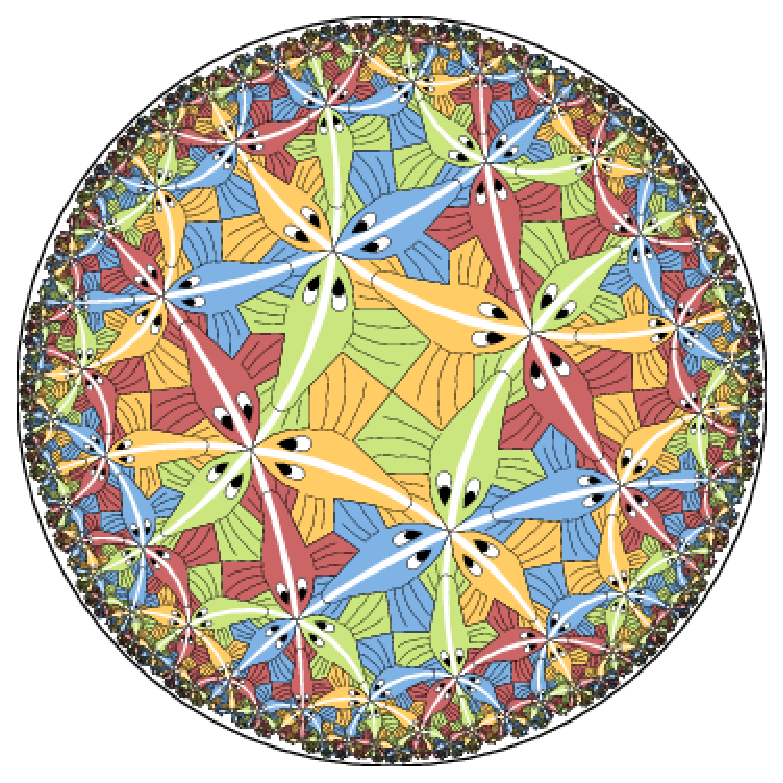
\includegraphics{circlelimit}}
\caption{A re-creation of Escher's \emph{Circle Limit III}, 
a depiction of hyperbolic geometry on the Poincar\'e disc.
Taken from \cite{transhyp}.}
\label{fig:circlelimit}
\end{figure}

% \subsection{Space-Time Algebra}

\subsection{Spherical Geometry}

FIXME: Spherical chat

\section{Extending the Conformal Model}

In this section we shall extend the conformal model we have developed to
represent Euclidean geometry to the hyperbolic geometry of the Poincar\'e
disc and show how many results which are tedious to prove using existing
metric-based derrivations become simple and, in some cases, obvious using the
GA-based approach.

%\subsection{Spherical Geometry}
%
%FIXME: spherical rotors
%
\subsection{Hyperbolic Geometry}

All rigid-body transformation (i.e.\ rotation and translation) rotors in 
the Euclidean approach above leave $n$ invariant, i.e.\ 
$Rn\tilde{R} = n$ for all rotors $R$. They also leave $\bar{n}$ invariant. We have
already identified $n$ and $\bar{n}$ with the points at infinity and the origin 
respectively. The question arises: `What if we restrict rotors to keep other
vectors invariant?'. Since a geometry is defined by its congruence transformations,
changing those transformations will therefore reflect a different geometry.

Instead we choose to restrict the rotors such that they keep $e$
invariant. Without loss of generality, we deal with a conformal extension of
$\mathbb{R}^2$ and write down a set of four basis vectors
\begin{equation}
E_1 = e_1 \quad E_2 = e_2 \quad E_3 = e \quad E_4 = \bar{e}
\end{equation}
and thus form the rotors $R_{k\ell } = \exp\left(\frac{\alpha}{2}E_k \wedge E_\ell\right)$ with $k,\ell \in \{1,2,3,4\}$.
Applying them to $e$ via $R_{k\ell }e\tilde{R}_{k\ell } \equiv R_{k\ell }eR_{\ell k}$ we find
the bivector generators of the rotors which preserve $e$ are $\bar{e}e_1$, 
$\bar{e}e_2$ and $e_1e_2$. The latter just correspond to rotations in the
$e_1e_2$ plane and hence, the former two must be the generators of
translations. We can say, therefore, that a rotor which translates the origin to the vector
$x$ must be given by a multivector of the form
\begin{equation}
T_x = \exp\left(\frac{f(r)}{2}\bar{e}\hat{r}\right)
\end{equation}
where $r = |x|$, $\hat{r} = x/|x|$ and $f(r)$ is some function of $r$ yet to
be determined. Noting that $(\bar{e}{e_1})^2 = (\bar{e}e_2)^2 = +1$ and therefore
$(\bar{e}\hat{r})^2 = +1$ we can take the power series expansion of $T_x$ and
collect like-coefficients to obtain
\begin{equation}
T_x = \cosh\left(\frac{f(r)}{2}\right) + \bar{e}\hat{r}\sinh\left(\frac{f(r)}{2}\right)
\label{eqn:nonEuclidTrans1}
\end{equation}

The choice of the origin is only restricted in that it must differ from the 
point at infinity and must not contain components of $e_1$ or $e_2$ (to retain
isotropy). Either $n$ or $\bar{n}$ is a suitable choice but we choose
a multiple of $\bar{n}$
to retain compatibility with the Euclidean case.

Again, as with the Euclidean case, we wish to impose a normalisation condition 
on the null-vectors, 
$X = F_e(x)$, such that 
\begin{equation}
X \cdot e = -1
\end{equation}
where we use $F_e(x)$ to represent the mapping defined by the geometry
generated by the rotors which
preserve $e$. If this is to hold then the origin must in fact be $-\bar{n}$.

We can now find the representation of the general point $x$ as the translation
along $x$ of the origin. Writing $c = \cosh\left(\frac{f(r)}{2}\right)$ and
$s = \sinh\left(\frac{f(r)}{2}\right)$
\begin{eqnarray}
F_e(x) & = & T_x\,(-\bar{n})\,\tilde{T}_x \\
& = & \left[c + \bar{e}\hat{r}s\right] (-\bar{n}) \left[c - \bar{e}\hat{r}s\right] \\
&=& -c^2\bar{n} + 2sc\hat{r} + s^2n 
\end{eqnarray}
then letting $C = \cosh(f(r))$ and $S = \sinh(f(r))$ giving $c^2 = (C+1) / 2$,
$s^2 = (C-1)/2$, $sc = S/2$ and hence
\begin{eqnarray}
F_e(x) & = & \frac{1}{2}n (C-1) - \frac{1}{2}\bar{n}(C+1) + S\hat{r} \\
& = & \frac{1}{2} \left[ \, (C-1)n + 2S\hat{r} - (C+1)\bar{n} \, \right] 
% & = & \frac{1}{2} \left[ \, (\cosh(f(r))-1)n + 2\sinh(f(r))\hat{r} - (\cosh(f(r))+1)\bar{n} \, \right] 
\end{eqnarray}
As required $(F_e(x))^2 = 0$ and $F_e(x) \cdot e = -1$.

It remains to choose a sensible form for $f(r)$. We seek to choose $f(r)$ such that
the representation $F_e(x)$ is similar to our Euclidean representation $F(x)$
since this will allow us to use many of the same techniques we developed for the
Euclidean case. We can re-write our Euclidean representation 
in terms of $r$ and $\hat{r}$ as
\begin{equation}
F(x) = \frac{1}{2\lambda^2}(r^2n + 2 \lambda r\hat{r} - \lambda^2\bar{n})
\label{eqn:nonEuclidMap1}
\end{equation}

If we wish that $F_e(x)$ be similar to $F(x)$ then we have the conditions
\begin{equation}
\frac{S}{C + 1} = \frac{\sinh(f(r))}{\cosh(f(r)) + 1} = \frac{r}{\lambda}
\label{eqn:rlambda}
\end{equation}
and
\begin{equation}
\frac{C-1}{S} = \frac{\cosh(f(r)) - 1}{\sinh(f(r))} = \frac{r}{\lambda}
\label{eqn:rlambda2}
\end{equation}
so the mapping function becomes
\begin{eqnarray}
F_e(x) &=& \frac{C+1}{2\lambda^2}\ [x^2n + 2\lambda x - \lambda^2 \bar{n}] \\
&=& \frac{\cosh(f(r)) + 1}{2\lambda^2}\ [x^2n + 2\lambda x - \lambda^2 \bar{n}]
\end{eqnarray}
which has a degree of similarity to the expression for $F(x)$. Further, 
assuming $r$ and $\lambda$ are positive, we can see from equation
\ref{eqn:rlambda} that $r < \lambda$ since $\sinh(A) < 1 + \cosh(A)$
for all $A$.

Given equations \ref{eqn:rlambda} and \ref{eqn:rlambda2}, we can eliminate
$\sinh(f(r))$ to give
\begin{equation}
\frac{\cosh(f(r)) -1}{\cosh(f(r)) + 1} = \frac{r^2}{\lambda^2}
\end{equation}
and hence $\cosh(f(r)) = (\lambda^2 + r^2)/(\lambda^2 - r^2)$. Substituting
into either \ref{eqn:rlambda} or \ref{eqn:rlambda2} gives
\begin{equation}
f(r) = \sinh^{-1}\left( \frac{2\lambda r}{\lambda^2 - r^2} \right)
\end{equation}
and hence we can form the following expressions for 
$\sinh(f(r))$ and $\cosh(f(r))$
\begin{equation}
\sinh(f(r)) = \frac{2\lambda r}{\lambda^2 - r^2} \quad \mbox{ and } \quad
\cosh(f(r)) = \frac{2\lambda^2}{\lambda^2 - r^2} - 1
\end{equation}

Inserting these into equation \ref{eqn:nonEuclidMap1} gives the final form
of the non-Euclidean mapping function
\begin{equation}
F_e(x) = \frac{1}{\lambda^2 - x^2}(x^2 + 2\lambda x - \lambda^2\bar{n})
\label{eqn:nonEuclidMapping}
\end{equation}

We can also show, by substituting the results in equation \ref{eqn:sinhcosh}, 
that the form of the translation rotor given in 
equation \ref{eqn:nonEuclidTrans1} can also be written as
\begin{equation}
T_x = \frac{1}{\sqrt{\lambda^2 - x^2}}(\lambda + \bar{e}x)
\label{eqn:transrotor}
\end{equation}

Some discussion of the relevance of $\lambda$ is worthwhile here. Notice that
in order for the translator to remain real-valued, $x^2 \le \lambda^2$. 
We can never therefore translate the origin outside of a circle radius
$\lambda$ centred upon it. The value of $\lambda$ effectively defines
a region of inaccessible space from the origin, effectively a boundary to
the geometry.

This circle corresponds directly to the unit-circle boundary in the
Poincar\'e disc representation if $\lambda = 1$ and simple dilations of
the Poincar\'e representation if $\lambda \ne 1$. To maintain compatibility
with the Poincar\'e representation, we usually set $\lambda$ to be unity.

%
The rotor in equation \ref{eqn:transrotor} is, by construction, the rotor 
which takes us from
the origin to position $x$. A difference from the
Euclidean case is that now $T_x$ and $T_y$ do not commute
for two different positions $x$ and $y$. This means that
$T_{y-x}$ is {\em not\/} the rotor taking us from
position $x$ to position $y$. However, this is not a
problem, since we can always achieve this motion via
going back through the origin, and forming
%
\begin{equation}
T_{x \mapsto y} = T_y T_{-x}
\end{equation}
%
Since composition of rotors always produces another
rotor, this means that we have the same freedom as in the
Euclidean case to prove a relation we are interested in,
at some special position and orientation, and then use
the covariant rotor structure to generalise the result to
general positions and orientations. Spatial rotations are
of course achieved as before with rotors of the form
$R=\exp\left(\frac{\theta}{2}e_1 e_2\right)$.

The final motion we should consider is the analogue of
inversion. Unlike in the Euclidean case, inversion using
reflection in $e$ is now a fully covariant operation.
Specifically, if $R$ represents any combination of
rotation and translation, and $A$ is some object in the
space, we have
%
\begin{equation}
eAe \mapsto Re\tilde{R}\, RA\tilde{R}\, Re\tilde{R} = e
RA\tilde{R} e = R(eAe) \tilde{R}
\end{equation}
%
The last equality means that transforming $A$ first and
then reflecting is the same as reflecting and then
transforming, which is what is required of a covariant
operation. The availability of this reflection operation
is very useful. The translation rotors discussed above
clearly only allow us to move around within the interior
of the disc $r<\lambda$. By reflection in $e$, as we
shall see below, we are able to jump into a `dual world'
outside the disc.

Having achieved a representation function, and discussed
the set of motions, we should examine this new space in
relation to the Poincar\'e disc, which we have said it is
equivalent to. The first thing is to examine the distance
function, i.e. how we assign a non-Euclidean distance
function between points in the space.

If we consider a simple rotation,
$\exp\left(\frac{\theta}{2}\hat{B}\right)$, where $\hat{B}$ is some unit
spatial bivector, then we are used to the idea that
$\theta$ is the correct measure of distance (here
angular) to describe the transformation. Thus if we
consider again the translation rotor in
equation \ref{eqn:nonEuclidTrans1}, $T_x = \exp\left(\frac{f(r)}{2}\bar{e}\hat{r}\right)$,
%
%\begin{equation}
%T_x = \cosh(f(r)/2) + \ebar \rhat \sinh(f(r)/2) =
%\exp((f(r)/2) \ebar\rhat)
%\end{equation}
%
%where $f(r) = \sinh^{-1}\left(\frac{2\lambda
%r}{\lambda^2-r^2}\right)$,
we would expect the correct distance
measure to associate with it would be $f(r)$. This would be a
viable option, except that for points close to the origin of the
disc ($r\ll\lambda$) we would like ordinary Euclidean notions of
distance to apply, at least approximately. Now $\ebar =
(1/2)(n-\nb)$ and the $\nb$ part of this, when exponentiated and
applied as in equation \ref{eqn:almost-X-rep}, has no effect to
first order on the origin point $-\nb$, whereas the $n$ part does;
e.g.
%
\begin{eqnarray}
T_x(-\nb)\tilde{T}_x & \approx  & \left(1+
\frac{f(r)}{2}\frac{(n-\nb)\rhat}{2}\right)(-\nb)\left(1-
\frac{f(r)}{2}\frac{(n-\nb)\rhat}{2}\right)   \nn \\
 & =  &
\left(1+
\frac{f(r)}{2}\frac{n\rhat}{2}\right)(-\nb)\left(1 -
\frac{f(r)}{2}\frac{n\rhat}{2}\right)
\end{eqnarray}
%
This means that, to first order near the origin, the
$T_x$ rotor approximates in its actions the Euclidean
translation rotor corresponding to distance $f(r)/2$
rather than $f(r)$, i.e.
%
\begin{equation}
T_x \approx 1 + \frac{f(r)}{2}\frac{n \rhat}{2}
\end{equation}
%
For this reason, we take the non-Euclidean distance
between a point and the origin to be given by $f(r)/2$
rather than $f(r)$. Calling this non-Euclidean distance
function $d(r)$, and using equation
\ref{eqn:sinhcosh} along with the identity 
\[\sinh\left(\frac{z}{2}\right) =
\left[\frac{\cosh z - 1}{2}\right]^{\frac{1}{2}},\]
gives
%
\begin{equation} \label{eqn:defines-dofr}
d(r) =
\sinh^{-1}\left(\frac{r}{\sqrt{\lambda^2-r^2}}\right)
\end{equation}
%
We note this approximates to $r/\lambda$ for
$r\ll\lambda$, i.e. we recover the Euclidean distance
measured in units of $\lambda$.

This function gives us the distance of a point from the
origin, but what about the distance between two general
points, neither of which is at the origin? One of the
major advantages of the conformal approach to Euclidean
geometry is that it gives us an inner product formula for
computing the distance between any two points, and we
would hope that the same would be possible here. This is
indeed the case. Let $X$ be the null vector corresponding
to the point $x=r\, \rhat$ using our representation,
equation (\ref{eqn:nonEuclidMap1}). Then, since $n\dt\nb =
2$, we can rewrite eqn~(\ref{eqn:defines-dofr}) as
%
\begin{equation} \label{eqn:dist-to-origin}
d(r) = \sinh^{-1}\left(\sqrt{-\frac{1}{2} X \dt (-\nb) }
\right)
\end{equation}
%
Note, $X \dt (-\nb)$ is the inner product of $X$ with the
null vector representing the origin. Two points in any
general positions can be wound back using a common
translation rotor so that one of them ends up at the
origin. For example, let $T_y$ be the translation rotor
that takes $Y$ back to the origin, then
%
\[ X' = T_y X \tilde{T}_y \qquad  Y' = T_y Y \tilde{T}_y
= -\nb
\]
%
so that $X'\dt Y' = (T_y X \tilde{T}_y)\dt T_y Y \tilde{T}_y =
X\dt Y =  X'\dt (-\nb)$. Since we know that a function of $-\half
X'\dt (-\nb)$ gives the distance between the two points from
equation~(\ref{eqn:dist-to-origin}), we can now write this
distance in terms of $X\dt Y$. Note that at no stage in the
process is the inner product between the null vectors changed (the
inner product is rotor invariant), and thus we have succeeded in
defining a distance between general points in terms of inner
products. If the general points are $x$ and $y$ with
representatives $X$ and $Y$, the expression for the distance
function is thus
%
\begin{equation}\label{eqn:general-dist-formula}
d(x,y) = \sinh^{-1}\left(\sqrt{-\frac{1}{2} X \dt Y }
\right)
\end{equation}
%
which is a satisfyingly simple relationship. As in the
Euclidean case, it is a monotonic function of $X\dt Y$.
If we take the inner product of $X$ and $Y$ we obtain,
using equation~\ref{eqn:nonEuclidMap1},
%
\begin{eqnarray}
X\dt Y  & = &
\frac{1}{(\lambda^2-x^2)(\lambda^2-y^2)}\left[-2\lambda^2x^2-2\lambda^2y^2+4\lambda^2xy\right] \nn \\
  &  =  &
  \frac{-2\lambda^2}{(\lambda^2-x^2)(\lambda^2-y^2)}(x-y)^2
  \end{eqnarray}
%
Written in terms of the points themselves the distance
between the points is therefore
%
\begin{equation}\label{eqn:general-dist-formula-points}
d(x,y) = \sinh^{-1}\left(\lambda
\sqrt{\frac{(x-y)^2}{(\lambda^2-x^2)(\lambda^2-y^2)} }
\right)
\end{equation}
%

Armed with this distance function, we can now investigate
geodesics in the disc. These are the lines that are `straightest'
in the geometry defined by the distance function (more precisely,
the arc length along them is extremal.) We will not give the
details, but show some numerically computed examples in
Fig.~\ref{fig:hyper-geos}.
%
\begin{figure} \label{fig:hyper-geos}
\centerline{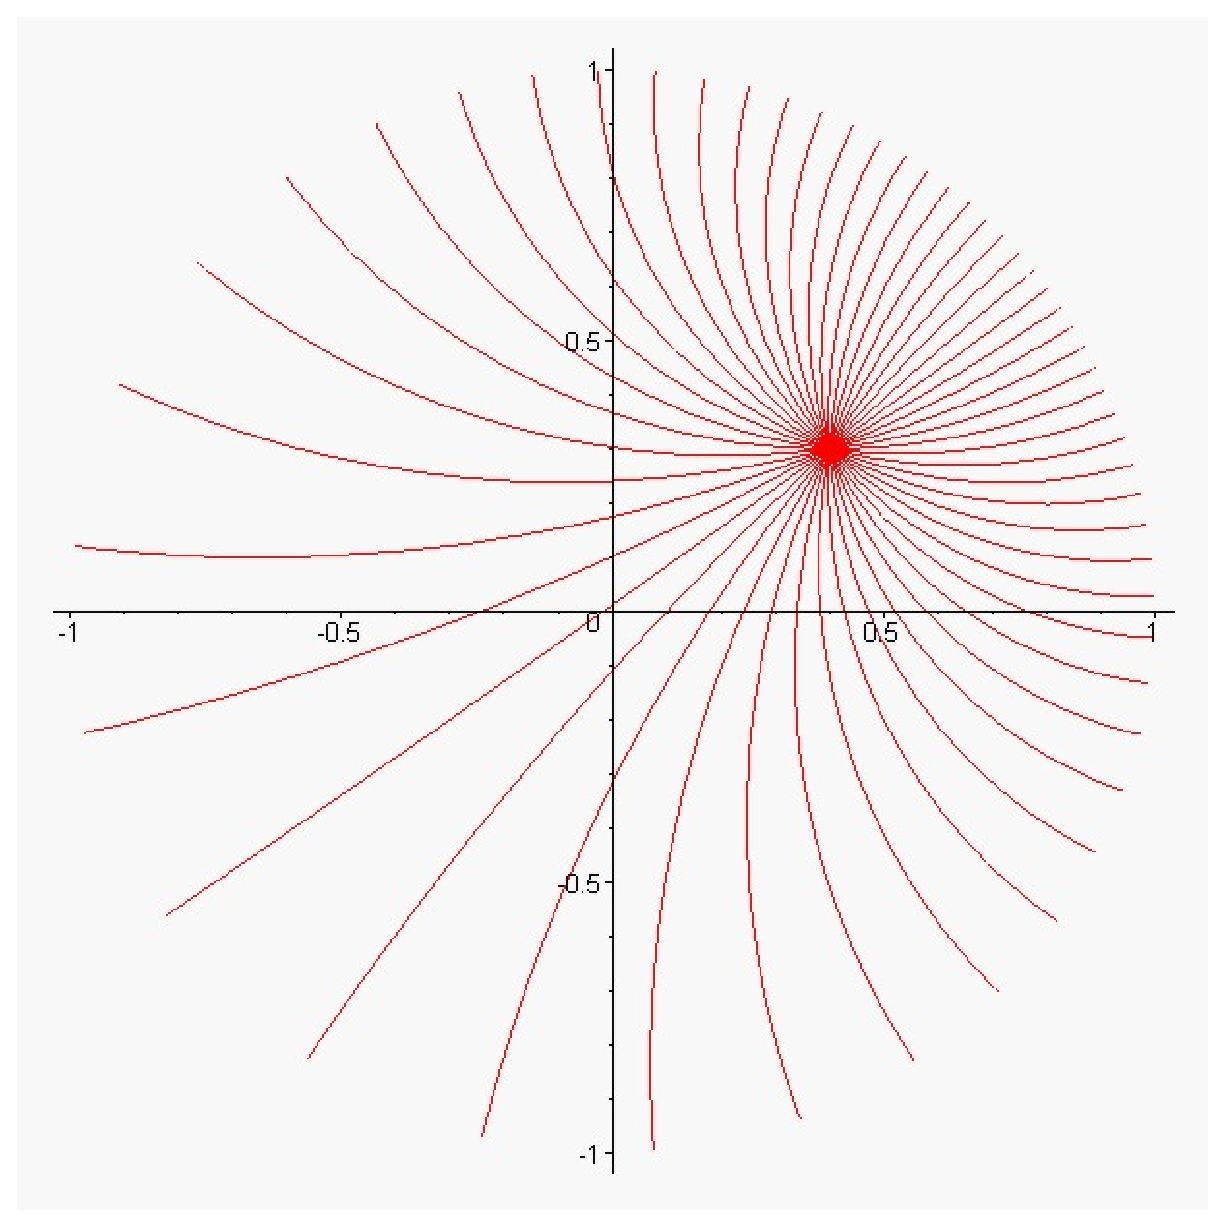
\includegraphics[width=0.5\textwidth]{hyper_geos}}
\caption{Geodesics emanating from a point in hyperbolic space.
They all intersect the unit circle at right angles and each is in
fact the arc of a circle. ($\lambda=1$ has been taken here.) }
\end{figure}
%
In calculating these we have taken $\lambda=1$, so the disc is now
the unit disc ordinarily considered in the Poicar\'e model. One
finds that each geodesic is an arc of a circle, and that each of
them asymptotically approaches the bounding unit circle at right
angles. At this point we can start making contact with the
description of the classical approach to the Poincar\'e disc given
in \cite{GEOM:brannan}. The geodesics there are called {\em $d$-lines}.
They are not justified in terms of being geodesics, but simply
defined as being arcs of circles which cut the boundary at right
angles. However a distance function is given in \cite{GEOM:brannan}, which
in terms of distance to the origin is
%
\begin{equation}
d(x,0) = \tanh^{-1}(|x|)
\end{equation}
%
and therefore agrees with our identification of $d(r)=
f(r)/2$, using equation (\ref{eqn:sinhcosh}), and
taking $\lambda=1$.

Thus far, apart from the formula for non-Euclidean
distance in terms of $X \dt Y$, we have only mirrored
what is already known. We now start to show the power of
the conformal GA approach to this geometry, by showing
how the operations and objects defined previously in
conformal Euclidean geometry have immediate analogues
here, representing a considerable unification, and saving
of effort. It may also be worth noting here that the
power of this approach extends immediately to 3
dimensions. All the above formulation, and what we do
next, transfers seamlessly to 3d, where the Poincar\'e
disc becomes a ball. All the formulae are correct already
for this transition. On the other hand, to provide a
computational scheme which is somewhat akin to our rotor
formulation, Brannan \emph{et al} \cite{GEOM:brannan} introduce complex coordinates
to work in the Poincar\'e disc, and use Mobius
transformations in place of the rotors. These are
effective computationally in 2d, but of course the
complex variable apparatus does not extend at all to 3d
(unless one uses the GA approach!). Also of course, the
conformal setup enabling points, lines, circles, spheres
and planes to be integrated into one algebraic system
does not exist in the complex variable approach, even in
2d.

\subsection{Geometric Objects in Hyperbolic Geometry}

\subsubsection{Hyperbolic lines}

Having dealt with distances between points, let us start with the
next most fundamental objects --- lines. In Euclidean space we
have seen that these are given by $L = n \wedge A \wedge B$, where $A$
and $B$ are (the representatives of) any two points on the line.
Rotor transformations are able to move lines around successfully
because for either a rotation or translation, $R n \tilde{R} = n$.
Thus when we perform $R L \tilde{R}$ we end up with $n \wedge (R A \tilde{R})
\wedge (R B \tilde{R})$ which is a line through the transformed points.
(Dilations also fit into this, since although they introduce a
scale factor when acting on both $n$ and general points, this
still produces the intended line up to a scale factor in the
Euclidean case.)

This discussion makes it clear what a line must be in the
conformal approach to hyperbolic geometry. Instead of
using $n$, we must use the invariant object $e$. Thus we
define a hyperbolic line as
%
\begin{equation}\label{eqn:line-def}
L = e \wedge A \wedge B
\end{equation}
%
where $A$ and $B$ are the two points through which we
wish it to pass. This construction will guarantee
covariance of the definition of a line, for the same
reasons as in the Euclidean case (namely here that $R e
\tilde{R} = e$ for any allowable rotor $R$).

The immediate, very important question, of course, is
what precisely {\em is\/} the object we have constructed.
Ideally it should correspond to the $d$-line geodesics we
have just discussed. To determine whether a position $X$
lies on this line, we need to solve $X\wedge L=0$. Let us
take $x=x_1 e_1 + x_2 e_2$, $a=a_1 e_1 + a_2 e_2$ and
$b=b_1 e_1 + b_2 e_2$. Then, taking $\lambda=1$ for
convenience,  it is easy to show the resulting equation
for $x$ is of the form
%
\begin{equation}\label{eqn:brannan-d-line}
x_1^2+x_2^2-2 p x_1 -2 q x_2 +1 =0
\end{equation}
%
where $p^2+q^2>1$. Specifically, one finds
%
\begin{align}
p &= -\frac{1}{2}\,\frac {\left\{({a_1}^2+{a_2}^2
+1)\,b_2 - ({b_1}^2+{b_2}^2 +1)\,a_2\right\}}{ a_1\, b_2-
a_2\, b_1} \nn \\
%
q &= -\frac{1}{2}\,{\frac {\left\{-({a_1}^2+{a_2}^2
+1)\,b_1 + ({b_1}^2+{b_2}^2 +1)\,a_1\right\}}{{ a_1}\,{
b_2}-{ a_2}\,{ b_1}}} \nn
%
\end{align}
%
Equation (\ref{eqn:brannan-d-line}) is precisely the form
of equation given for $d$-lines in \cite{GEOM:brannan} page 283 and shows that
indeed our recipe in terms of wedging with $e$ has worked.

We can combine the notions of lines and distance, by asking for
the `hyperbolic midpoint' of the line segment joining two
positions $a$ and $b$. This is that point lying on the $d$-line
between $a$ and $b$ which is an equal hyperbolic distance from
each. Brannan \emph{et al} deal with this on page 288\cite{GEOM:brannan}, but consider only
the easiest case where the two points lie along a diameter of the
unit disc.

We know in the Euclidean case, that forming $A+B$ will give a
non-null point consisting of a multiple of the null vector
representing the desired midpoint, plus a multiple of the point at
infinity $n$. We hypothesise that we will get the same behaviour
here, but with $e$ playing the role of $n$. We can use two
different methods to obtain these results. The second is faster
than the first, but we outline both, since they both typify the
techniques available for use, and serve as good illustrations of
the power of the covariant method for hyperbolic geometry.

Firstly, since we can move objects around at will, let us
establish the result in the simplest case, where the two
points are symmetrically disposed about the origin, e.g.
let $a=\alpha e_1$ and $b=-\alpha e_1$. Clearly, by
symmetry the hyperbolic midpoint must be the origin
itself, so we write
%
\begin{equation} \label{eqn:mid-point-requirement}
A+B = \beta (-\nb) + \delta e
\end{equation}
%
where $\delta$ and $\beta$ are scalar multiples to be determined.
Since $A+B = \frac{2}{\lambda^2 - \alpha^2}(\alpha^2 n - \lambda^2
\nb)$ it is easy to see that we must have
%
\begin{equation}
\delta = \frac{4\alpha^2}{\lambda^2-\alpha^2} \quad
\text{and} \quad \beta =
\frac{2(\alpha^2+\lambda^2)}{\lambda^2-\alpha^2}
\end{equation}
%
Meanwhile, we note that
%
\begin{equation}
A\dt B = -\frac{8 \alpha^2
\lambda^2}{(\lambda^2-\alpha^2)^2}
\end{equation}
%
and some straightforward manipulation then tells us that
%
\begin{equation} \label{eqn:delta-beta-results}
\delta=\sqrt{4-2 A\dt B} -2 \quad \text{and} \quad \beta
= \sqrt{4-2 A\dt B}
\end{equation}
%
We have by this means actually solved the general
problem! To see this, note that we can now rearrange
equation (\ref{eqn:mid-point-requirement}) to get
%
\begin{equation}
-\nb = \frac{1}{\sqrt{1-\frac{1}{2} A \dt B}} \left\{
\frac{1}{2} (A+B) - e \left(\sqrt{1-\half A \dt
B}-1\right) \right\}
\end{equation}
%
Everything on the r.h.s. is covariant, and the separation between
$A$ and $B$ was controlled by a variable which was kept general
($\alpha$), so by employing translation and rotation rotors on the
r.h.s. we can make $A$ and $B$ line up with any two desired
points. Meanwhile the l.h.s. will keep track, and must still
remain the midpoint. (To see this, note that its `dot' with the
new points that $A$ and $B$ transform into, will remain constant
during this process.) The $e$ term just remains invariant. For two
completely general points $A$ and $B$ therefore, their
hyperbolic midpoint is given by
%
\begin{equation} \label{eqn:mid-point-expr}
X_{\rm mid} = \frac{1}{\sqrt{1-\frac{1}{2} A \dt B}}
\left\{ \frac{1}{2} (A+B) - e \left(\sqrt{1-\half A \dt
B}-1\right) \right\}
\end{equation}
%
which is a fully covariant expression.

The alternative method, which is quicker computationally, is as
follows. Let us write equation (\ref{eqn:mid-point-requirement})
again but this time with $X_{\rm mid}$ in place of $-\nb$ and with
a general $A$ and $B$ in place from the beginning. So
%
\begin{equation}
A+B = \beta \, X_{\rm mid} + \delta e
\end{equation}
%
Rearranging, we have
%
\begin{equation}
X_{\rm mid} = \frac{1}{\beta} (A+B-\delta e)
\end{equation}
%
which shows that our assumption about the form of the
midpoint is in fact valid. This is because dotting the
r.h.s. with $A$ and $B$ in turn, we obtain
%
\begin{equation}
X_{\rm mid} \dt A = X_{\rm mid} \dt B = \frac{1}{\beta}
(A\dt B+\delta)
\end{equation}
%
This means that $X_{\rm mid}$ is indeed equidistant, in a
hyperbolic sense, from $A$ and $B$. Moreover,
%
\begin{equation}
X_{\rm mid} \wedge (e \wedge A \wedge B) = 0
\end{equation}
%
so it correctly lies on the $d$-line joining them.

It just remains to fix $\delta$ and $\beta$ via requiring
that $X_{\rm mid}$ is null and is correctly normalised.
The null requirement gives
%
\begin{equation}
2 A \dt B + 4 \delta + \delta^2 = 0
\end{equation}
%
and requiring $X_{\rm mid} \dt e = -1$ yields
%
\begin{equation}
\beta=\delta+2
\end{equation}
%
Solving these yields (\ref{eqn:delta-beta-results}) as
before, and we recover (\ref{eqn:mid-point-expr}).

\subsubsection{Hyperbolic circles}

A great deal of hyperbolic geometry is concerned with
hyperbolic circles, i.e. the locus of points that are
at a constant hyperbolic distance from a given centre.
We can immediately hypothesise that such a circle,
passing through the points $A$, $B$, $D$  should be given
by the trivector.
%
\begin{equation}
C = A \wedge B \wedge D
\end{equation}
%
Thus the set of points $X$ which satisfy $X\wedge C=0$ can be found
from the Euclidean case, since we have the same null points being
wedged together here, up to scale, and this will not affect the
outcome (e.g.\ in the Euclidean case we know that $X =
\frac{1}{2\lambda^2}[x^2n + 2\lambda x - \lambda^2\nb]$ and in the
hyperbolic case $X = \frac{1}{\lambda^2 - x^2}[x^2n + 2\lambda
x - \lambda^2\nb]$). If the above hypothesis is true, we can
immediately deduce the somewhat surprising, though in fact true,
conclusion that hyperbolic circles are also Euclidean circles.
It turns out that it is just their centres that are in general
different.

To establish that $C$ is a hyperbolic circle (as well as
clearly a Euclidean one) we can take the special case of a circle
centred at the origin. By symmetry, this must be both a Euclidean
and hyperbolic circle. Let this have Euclidean radius $\rho$.
If we recall our earlier work, then for the scaled version of the
null point representative, the inner product between two points
$A$ and $B$ is given by
%
\begin{equation}
     A\dt B = -\frac{1}{2\lambda^2}(a-b)^2
     \end{equation}
%
Then, since $X\dt B = -\frac{1}{2\lambda^2}(x-b)^2 =
-\frac{1}{2\lambda^2}(\rho)^2$ for a circle centre $B$ and radius
$\rho$, we have that
%
\begin{equation}
  X\dt (B-\frac{1}{2\lambda^2}(\rho)^2n)=0
\end{equation}
%
giving $C^*=B-\frac{1}{2\lambda^2}(\rho)^2n$, where $C$ is the
trivector describing the circle. Thus if $B$ is the origin, so
that $B = -\frac{1}{2}\nb$, the dual of $C$ is given by $C^* =
-\frac{1}{2\lambda^2}\{\rho^2 n + \lambda^2\nb\}$. Now, since
$n+\nb = 2e$ we can write $\rho^2 n + \lambda^2\nb$ as
%
\begin{equation} \label{eqn:dual-to-C}
\rho^2 n + \lambda^2 \nb = 2 \rho^2 e + (\lambda^2 -
\rho^2) \nb
\end{equation}
%
We can normalise this to $C^2=(C^{*})^2=1$ via the scaling
\[C^* \mapsto \alpha(\rho^2n + \lambda^2\bar{n})\quad\mbox{such that}
\quad(C^{*})^2 = 1
\]
and hence $\alpha = \frac{1}{2\rho\lambda}$, thus
\begin{equation}
C^* = \frac{1}{2 \rho \lambda} \left(\rho^2 n + \lambda^2 
\nb\right)
		=
\frac{1}{2\rho\lambda}[2\rho^2e + (\lambda^2 - \rho^2)\bar{n}].
\end{equation}
%
This displays the dual to $C$ as a linear combination of
the vector representing the origin, which is here the
centre of the circle, and a multiple of $e$. This is the
covariant form we require for generalisation. Note
%
%
\begin{equation}
X \dt (IC) = \frac{1}{2 \rho \lambda} \left\{ X \dt (2 \rho^2 e +
(\lambda^2 - \rho^2) \nb) \right\} = \frac{1}{2 \rho \lambda}
\left\{ -2\rho^2 -(\lambda^2-\rho^2) X \dt (-\nb) \right\}
\end{equation}
%
shows us how $X$ maintaining a constant hyperbolic distance
from the centre ($-\nb$) is guaranteed by $X \dt (IC)=0$, in which
case we have
%
\begin{equation}
X \dt (-\nb) = \frac{-2\rho^2}{(\lambda^2 - \rho^2)}
\end{equation}
%
Let us act on $IC=I(A \wedge B \wedge D)$ with hyperbolic rotors,
to move the 3 points around as we wish. These same rotors acting
on the right hand side of (\ref{eqn:dual-to-C}) mean that we will
continue to get the required behaviour of constant hyperbolic
distance from the transformed centre, since the rotors will take
the origin to the new centre of the circle, say $P$. Thus indeed,
the wedge of 3 points generates a hyperbolic circle, and
moreover the above enables us to extract its (hyperbolic)
radius and centre from the dual object. Again we see that the
r\^ole of the $n$ appearing in the Euclidean expressions is
replaced by $e$ here. Specifically we find the following: the
(normalised dual to the) hyperbolic circle with hyperbolic
centre $P$, Euclidean radius $\rho$ and hyperbolic radius $d$,
is given by
%
\begin{equation}\label{eqn:non-e-circle}
IC = \frac{1}{2 \rho \lambda} \left( 2 \rho^2 e +
(\rho^2-\lambda^2) P \right)
\end{equation}
%
with $d= \sinh^{-1} (\rho/\sqrt{\lambda^2-\rho^2})$, from
equation~\ref{eqn:general-dist-formula}.

\subsubsection{Hyperbolic reflection}

A very useful operation in hyperbolic geometry is the notion of
hyperbolic reflection, as defined for example in \cite{GEOM:brannan}. 
It is extremely easy to calculate the hyperbolic
reflection of a point $X$ in the $d$-line $L$ in the GA approach.
Assuming $L$ is normalised to satisfy $L^2=1$, we just form $LXL$,
the standard form of reflecting one object in another. Since $L e
L = e$ for any (normalised) line, we see that $X'=LXL$ is both
null and satisfies $X' \dt e=-1$ thus qualifying it to represent a
point. Moreover it is co-variantly constructed;
under a rotor transformation it just rotates to $R X'
\tilde{R}$ and thus must represent something physical. It is not
hard to show that the point it represents is that found by moving
along a $d$-line intersecting $L$ at right angles and passing
through $X$, by an equal hyperbolic distance on the other side
of the line as $X$ is on the original side. This is indeed the
definition of reflection in this case.

\subsection{Extension to Higher Dimensions and Other Geometries}

All the above transfers seamlessly to 3 and higher dimensions, in
most cases with no changes at all to the formulae. This is in
contrast to e.g. the methods introduced in \cite{GEOM:brannan}, which
rely on standard complex analysis and so only work in the 2d
plane. Furthermore, we can extend all the above analysis to the
case of \textit{spherical geometry} as well. This involves
replacing the role of $e$ with that of $\bar{e}$, which changes
some trigonometric functions and ranges of applicability, but
otherwise most of the above discussion goes through unchanged.

% \subsection{Space-Time Algebra}

\section{Non-Euclidean Visualisation Methods}
\subsection{NURBs}

A key requirement for visualising objects in the Poincar\'e disc
representation of hyperbolic geometry is to plot representations of
straight lines, known as $d$-lines. This chapter outlines a method 
developed to draw them using OpenGL and also presents a generalisation
of the method for drawing analogous `$d$-planes' in three-dimensional
hyperbolic geometry.


The $d$-lines on the Poincar\'e disc are circular arcs (and straight lines
for the special cases of lines through the origin). OpenGL, the graphics
library used for the implementation, has native support for a class
of curves called \emph{NURBS} (Non-uniform Rational B-Splines) 
\cite{mecg}. 

%It is
%not the r\^ole of this report to provide a complete tutorial on NURBS,
%suffice it to say that they provide a way of parametising a large class of
%curves by a set of \emph{control points} and associated \emph{weights}.

NURBS curves are specified using a set of control points, $P_i$,
weights, $w_i$ and a set of normalised basis functions $N_{i,k}$.
The curve is given by
\[
C(u) = \frac{\sum_{i=0}^n w_i P_i N_{i,k}(u)}{\sum_{i=0}^n w_i N_{i,k}(u)}
\]

The basis functions are defined recursively:
\[
N_{i,k}(u) = \frac{u - t_i}{t_{i+k} - t_i} N_{i,k-1}(u) +
  \frac{t_{i+k+1} - u}{t_{i+k+1} - t_{i+1}} N_{i+1,k-1}(u)
\]
with
\[
N_{i,0} = 
\begin{cases}
1 \mbox{ if } t_i \le u \le t_{i+1} \\ 
0 \mbox{ otherwise} 
\end{cases}
\]
and $t_i$ being the elements of the \emph{knot vector}
\[
U = \{ t_0, t_1, ... , t_m \}
\]

The relation between the number of knots, $m+1$, the degree $k$ of 
the functions $N_{i,k}$ and the number of control points, $n+1$
is given by $m = n + k + 1$ \cite{peigl, rogers}.

Clearly a large family of curves can be expressed with suitable choices
of knot vectors, weights and control points leading to great flexibility.
All NURBS curves share some common properties however which make them
useful in Computer Graphics. A NURBS curve \emph{always} stays inside the
convex hull of its control points \cite{rogers} and thus is is very easy
to compute whether the curve will be displayed at all. Further they
are tangential to the piece-wise linear interpolation of control
points and the end-points, see figure \ref{fig:samplenurb}.

\begin{figure} \centering
\scalebox{0.9}{\includegraphics{samplenurb}}
\caption{A set of control points and a typical example of an associated
NURBS curve. Note that the endpoints of the curve are tangential to
$P_0P_1$ and $P_5P_6$ and that the curve is within the convex hull
of the points (shaded).}
\label{fig:samplenurb}
\end{figure}

\subsection{Rendering $d$-lines}

To draw $d$-lines on the Poincar\'e disc, we wish to draw circular arcs
with end-points on the boundary circle and erupting normal to it.

A large number of different curves can be created with different control 
point numbers, positions and weights. Fortunately there are a number of
standard techniques to generate common curves. One such method of
drawing arcs is useful to us. We use three control
points; one at the start of the circular arc, one at the origin of the
boundary circle and one
at its end, see figure \ref{fig:nurbs}. 
The end-point weights are unity whereas the weight of the control
point at the origin is $\cos \gamma$ where $\gamma$ is the angle
$OA$ makes with $AB$\footnote{See http://www.ddt.pwp.blueyonder.co.uk/evgeny/Intro/NURBS.htm for a demonstration of this.}. 

\begin{figure} \centering
\scalebox{0.7}{\includegraphics{nurbs}}
\caption{NURBS-based rendering of $d$-lines. Here $O$ is the origin and
$A$ and $B$ are the boundary points of the line $L$.}
\label{fig:nurbs}
\end{figure}

Since NURBS are tangential to the piecewise linear interpolation of control 
points
at either end, it is clear that the curve erupts from the boundary
tangential to the lines $OA$ and $OB$. Given $O$ is the origin, and the
boundary is centred upon it, these lines are radii of the boundary
circle and so clearly are normals.

This allows us to construct a NURBS representation of any $d$-line
on the Poincar\'e disc (including diameters) and efficiently draw them
using OpenGL. 

\subsubsection{Calculating properties of $d$-lines}

The last step in drawing out $d$-lines is now finding where they intersect
the boundary disc, their \emph{boundary points}. 
Once we have these points, the drawing can be performed
via our NURBS-based method outlined above.

We can calculate approximate boundary points of $d$-lines
by forming a circle 
corresponding to the boundary and finding the 
meet of the line with this circle. This gives the null-vector
representation of the boundary points $A$ and $B$ as the
bivector $A \wedge B$ as with circle/sphere intersections and the like.
We have already shown that this bivector can be factorised into $A$ and 
$B$ via the method of projectors.
We finally need to calculate the angle $\gamma$ which is a trivial
exercise in trigonometric geometry. 

Figure
\ref{fig:hyp1} shows the rendering of $d$-lines in action.
Here we have three $d$-lines created by rotating and translating the
diameter to form a hyperbolic triangle (central dark-shaded
region). Each of these lines were reflected in the other two to form 
a set of three reflected triangles (outer light-shaded regions). This
operation could be repeated to tile the space.

\begin{figure} \centering
\scalebox{0.5}{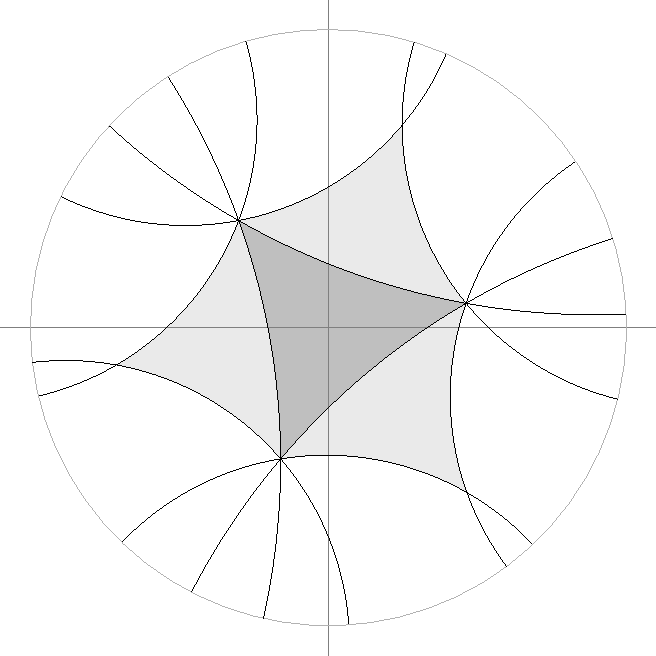
\includegraphics{hyperbolic1}}
\caption{NURBS rendering of $d$-lines in action.}
\label{fig:hyp1}
\end{figure}

\subsection{Rendering `$d$-planes'}


Drawing $d$-lines is interesting in itself but is an already solved 
problem many-times over. What is interesting is the generality the CGA
approach provides. Recalling our discussion of the development of
hyperbolic geometry in CGA, at no point did we ever assume only 
two-dimensions. We now have the intriguing opportunity to investigate
visualisation algorithms in three-dimensions.

We'll first assume that there is some analogous form to the Poincar\'e
disc representation for three-dimensions. In this case, $d$-lines can
be drawn using a similar method, this time intersecting them with a 
boundary sphere to find the two points of eruption. What would be 
more interesting is attempting to find the form for `$d$-planes'.

The method of defining planes in hyperbolic geometry is identical
to our definition in Euclidean geometry; given four points on the
$d$-plane, $\{ x_1, ..., x_4 \}$, the plane $\Phi$ is defined as
\begin{equation}
\Phi = \bigwedge_{i = 1...4} F_e(x_i)
\label{eqn:plane}
\end{equation}
Note we have incorporated the mapping into null-vectors within
the definition. Any point, $p$, which lies on the plane $\Phi$ satisfies
\[
F_e(p) \wedge \Phi = 0
\]

The drawing of $d$-planes is, however, less straight-forward. Firstly we
need to find what shape they are when represented in the Poincar\'e sphere.
Recall that
\[
F_e(x) = \frac{1}{\lambda^2 - x^2} (x^2 + 2\lambda x - \lambda^2\bar{n})
 =  \frac{2\lambda^2}{\lambda^2 - x^2} F(x)
\]
where $F(x)$ is the mapping function for Euclidean geometry. The factor
$(2\lambda^2) / (\lambda^2 - x^2)$ is always scalar for any vector
$x$ and we shall represent it as the function $s(x)$. Hence we can
re-write equation \ref{eqn:plane} as
\begin{eqnarray}
\Phi & = & \bigwedge_{i = 1...4} s(x_i)F(x_i) \\
     & = & \left[\prod_{i = 1...4} s(x_i)\right] \bigwedge_{i = 1...4} F(x_i) \\
     & = & S(x_1, x_2, x_3, x_4) \bigwedge_{i = 1...4} F(x_i) 
%%     & = & \left[\prod_{i = 1...4} s(x_i)\right] \Sigma
\end{eqnarray}

Now $\Phi$ is defined as the product of some scalar function, $S(...)$
of the defining points and the \emph{Euclidean} definition of a sphere. This
allows us to infer that, within the Poincar\'e sphere, a $d$-plane passing
through points $\{x_1, ..., x_4\}$ is represented by a sphere passing
through those same points.

\begin{figure} \centering
\scalebox{0.7}{\includegraphics{dplane}}
\caption{$d$-planes are caps of the corresponding Euclidean sphere.}
\label{fig:dplane}
\end{figure}

It has thus been found, without doing \emph{any} explicit calculations with
the metric, that
$d$-planes are represented in the Poincar\'e sphere by portions of spheres.
This neatly shows the analytical simplicity that this approach provides.
Figure \ref{fig:dplane} shows the
relation between $d$-planes and the corresponding Euclidean sphere.

%This nicely illustrates the analytical power that CGA provides us
%with. We have managed to obtain the form of a $d$-plane without
%resorting to complex extreemality calculations and, interestingly,
%without ever explicitly finding the metric. This suggests a powerful
%technique for inverstigating geometries where the geometry is well 
%known but the metric is awkward to deal with. The hyperbolic-tangent
%form for the metric in hyperbolic geometry is tedious to deal with
%analytically but we can infer important properties of the geometry
%intuitively with this approach.

We can find the meet between the associated Euclidean sphere and the
boundary sphere to give the circle of intersection. Inspecting figure
\ref{fig:dplane} we
see that this circle is the edge of the spherical
cap corresponding to the $d$-plane.

The spherical cap forming the $d$-plane can be thought of as the
intersection of the half-space containing the origin and bounded
by the plane of intersection (see figure \ref{fig:sphereplane}).
The circle of intersection is important since we wish to extract
this \emph{plane} of intersection efficiently. This is trivial
if we note that the circle is equivalent to the wedge-product of three
points on the circumference we can form the plane of the circle
by simply wedging the circle with $n$. In summary,
the plane of intersection, $P$ can be found from the $d$-plane $\Phi$ in
the following manner:
\[
P = k (\Phi \vee B) \wedge n
\]
where $B$ is the Euclidean representation of the boundary sphere
and $k$ is some scale factor.

\begin{figure} \centering
\scalebox{0.3}{\includegraphics{sphereplane}}
\caption{$d$-plane spherical cap is intersection of associated sphere and half-space
to right of plane $P$.}
\label{fig:sphereplane}
\end{figure}

Bajaj \emph{et al.} \cite{spherecap} provide a method of finding
a suitable set of control points and NURBS parameter space clipping
curve to draw spherical caps from sphere/half-space intersections.

Their approach gives a set of control points and weights that together
draw a little more than one hemisphere. Circular clipping paths in the 
parameter space are then used to form spherical caps.

This method was used to draw the spherical caps in the implementation.

% \section{Guidelines for Generalising Euclidean Algorithms}

well known fractals may be generated using Geometric Algebra. Further we show
how GA can be used to form a natural generalisation to higher dimensions and
non-Euclidean geometries. Some rendering strategies will also be discussed.

Fractals have always been a popular topic in computer graphics due to their
ability to give rise to great \ae sthetic beauty from a relatively simple
mathematical description. Generally a fractal is considered to be any
geometric object which possesses detail on all
scales\cite{FRAC:FractalsEverywhere, FRAC:FractalGeometryOfNature}. That is to
say, one may examine the edge of the object under arbitrary magnification
yet still find it rough and irregular. Many introductions to the subject of
fractals and their creation on computers exist elsewhere\cite{FRAC:FractalGeometry,
  FRAC:ChaosAndFractals, FRAC:FractalImages}.

The term fractal was coined by Mandelbrot\cite{FRAC:LesObjetsFractals} in 1975,
originally from the Latin {\em fractus} (broken) intended as a way of referring
to their edges which looks like jagged cracks in some surface. Since many
fractals (particularly those arising from so-caled \emph{Iterated Function Systems}) have
fractional Hausdorff dimension\cite{FRAC:GeometryOfFractalSets},
some have joked that `fractal' is actually a portmanteau word formed from
`fractionally' and `dimensional'.

Below we shall investigate an extension, via GA, of the class of fractals 
which is most associated with Mandelbrot -- those based on repeated iteration
of a complex function.  Similar fractals have found applications in a wide
selection of research areas including image 
compression\cite{Barnsley88c,Barnsley93b}.% and
%antenna design\cite{FRAC:Antennas}. 
It is hoped that the GA-based approach here may
also be of use in a similar manner however in this chapter we concentrate more
on the \ae sthetic nature of the fractals.

\section{Fractals from Complex Iteration}

\begin{figure}
\centering
\begin{tabular}{c@{$\quad$}c}
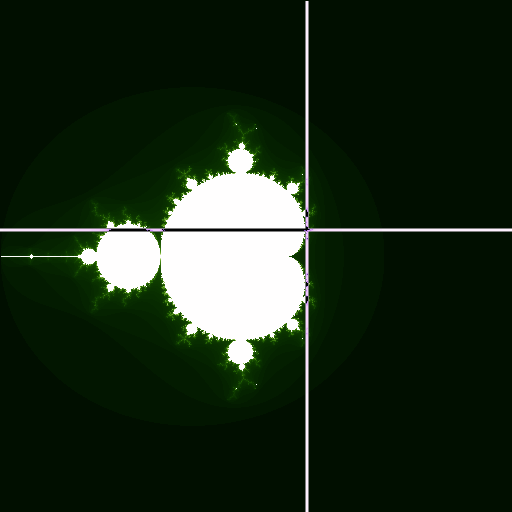
\includegraphics[width=0.4\textwidth]{euc_mandel_julia_pos} 
 & 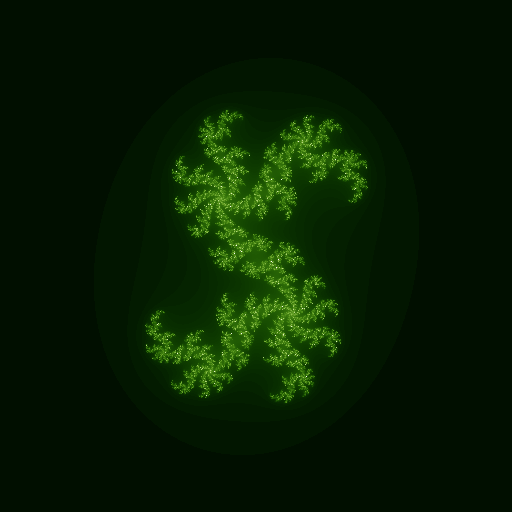
\includegraphics[width=0.4\textwidth]{julia_euc} \\
                          (a) & (b)
\end{tabular}
\caption{\label{fig:euclidean_sets}The well known (a) Mandelbrot set with
  the constant $c = 0.4 + 0.2i$ marked and (b) the Julia
  set associated with $c$.}
\end{figure}

The classical Mandelbrot and Julia sets (figure \ref{fig:euclidean_sets}) are
well known, even to laymen, as examples of fractals. They are
examples of a form of fractal known as \emph{recurrence} or 
\emph{escape-time}
fractals.  Such fractals are generated by iterating some complex function and
noting how fast it `escapes' to infinity (if at all).

Both fractals are displayed by mapping points in the complex plane to
pixels in the final image.
Usually this mapping to an image pixel location $\mathbf{x} = [\; x\;y \;]^T$
from its corresponding complex number, $c$, is simple.

\begin{definition}[Representation of the Complex Plane]
An image point $\mathbf{x} = [\; x\;y \;]^T$ is mapped to a point on the 
complex plane via that mapping $\mathbf{x} \mapsto {\mathcal I}(x)$ where
\[
{\mathcal I}({\mathbf x}) = [\; a_1 x + b_1 \; a_2 y + b_2 \;]^T
\]
and $(b_1,b_2)$ specify the origin of the area of interest in the complex
plane and $(a_1,a_2)$ specify its scale.
%\[
%{\mathcal I}(x) = [\; 1 \; i \;] \left[ 
%  \begin{array}{ccc}
%a & 0 & c \\
%0 & b & d \\
%  \end{array}
%\right]
%\left[
%  \begin{array}{c}
%  \mathbf{x} \\ 1
%  \end{array}
%\right].
%\]
%where constants $a,b,c$ and $d$ are set so as to specify 
%the area of the complex 
%plane shown in the image.
\end{definition}

The same complex function generates both the Mandelbrot and
Julia sets\cite{FRAC:Mandelbrot, FRAC:JuliaMandelBook}. It is worth noting
that other functions could be used and hence many other escape-time fractals
exist. In this chapter, to save space, we shall only consider developments from this function.

\begin{definition}
The complex function $f(z)$, $c \in {\mathbb C}$,
    is defined as
\[
f(z) = z^2 + c.
\]
\end{definition}

\begin{definition}[Iteration]
Iteration of a function $f(x)$ is denoted as $f^{(n)}(z)$ where
\[
f^{(n)}(z) \equiv f(f^{(n-1)}(z))
\]
and $f^{(0)}(z) \equiv z$, $n \in {\mathbb Z}^+$.
\end{definition}

\subsection{The Mandelbrot Set}

\begin{definition}[The Mandelbrot set]
The Mandelbrot set, $\mathbb{M}$, is defined as
\[
\mathbb{M} = 
\left\{c \in \mathbb{C} 
: \lim_{n \rightarrow \infty} \magof{f^{(n)}(0)} < \infty \right\} 
\]
where $\magof{z} \equiv (zz^*)^\frac{1}{2}$.
\end{definition}

\begin{lemma} 
\label{lem:convergence}
If $\magof{f^{(n)}(x)} \ge 2$
for some $n$ and $x$ then $\magof{f^{(n)}(x)} \rightarrow \infty$ as $n
\rightarrow \infty$.
\begin{proof}Suppose 
$\magof{f^{(n)}(x)} > 2$ and $\magof{f^{(n)}(x)} > \magof{c}$. It is
clear that
\[
\frac{\magof{f^{(n+1)}(x)}}{\magof{f^{(n)}(x)}} =
\frac{\magof{f^{(n)}(x)^2 + c}}{\magof{f^{(n)}(x)}}
\]
and hence
\[
\frac{\magof{f^{(n+1)}(x)}}{\magof{f^{(n)}(x)}} \ge 
\frac{\magof{f^{(n)}(x)}^2 - \magof{c}}{\magof{f^{(n)}(x)}} =
\magof{f^{(n)}(x)} - \frac{\magof{c}}{\magof{f^{(n)}(x)}}.
\]
As $\magof{f^{(n)}(x)} > \magof{c}$ and $\magof{f^{(n)}(x)} > 2$ then
\[
\magof{f^{(n)}(x)} - \frac{\magof{c}}{\magof{f^{(n)}(x)}} >
\magof{f^{(n)}(x)} - 1 > 1
\]
giving
\[
\frac{\magof{f^{(n+1)}(x)}}{\magof{f^{(n)}(x)}} \ge 1
\]
implying $\magof{f^{(n)}(x)} \rightarrow \infty$ as $n
\rightarrow \infty$ as required.
\end{proof}
\end{lemma}

Using lemma \ref{lem:convergence} we may determine if some point $x$ is
\emph{not} in the set as soon as $\magof{f^{(n)}(x)} \ge 2$.  In practise one
may have to wait an arbitrarily long time for this condition to be met and one
will never obtain it if $x$ is within the set. We approximate the set by
choosing some maximum number of iterations to wait before labelling $x$ as
being within the set.  Our algorithm for generating an image of the set is
shown in algorithm \ref{alg:generate_mandelbrot}.

\begin{fancyalg}
\begin{algorithmic}[1]
\STATE $i_{\mathrm{max}} :=$ maximum number of iterations
\FORALL{points $\mathbf{x}$ in image}
\STATE $c := {\mathcal I}(\mathbf{x})$
\STATE $z := c$
\STATE $i := 0$
\WHILE{$zz^* < 4$ and $i < i_{\mathrm{max}}$}
  \STATE $z := z^2 + c$
  \STATE $i := i+1$
\ENDWHILE 
\STATE set pixel $\mathbf{x}$ to colour $i$
\ENDFOR
\end{algorithmic}
\caption{
\label{alg:generate_mandelbrot}
  Generating the Mandelbrot set}
\end{fancyalg}

The level of detail of the resulting image being determined by the value of $i_{\mathrm{max}}$.
The image of the Mandelbrot set in figure \ref{fig:euclidean_sets}a was
generated with $\mathbf{x} = [\;x\;y\;]^T, x \in (-2,2), y \in (-2,2)$.
In figure \ref{fig:euclidean_sets}a a colour palette was also chosen such that colour 0 was black
and colour $i_{\mathrm{max}}$ was white moving through dark-green. The brightness of
each pixel is therefore some measure of how long it took to decide whether that point was
a member of the set.

\subsection{The Julia Set}

There are an infinite number of Julia sets; each point on the complex plane
has a corresponding Julia set. The definition of the Julia set is somewhat
similar to that of the Mandelbrot set.

\begin{definition}[The Julia set]
The Julia set, $\mathbb{J}_c$, associated
with the complex number $c$ is given by
\[
\mathbb{J}_c = 
\left\{z \in \mathbb{C}
: \lim_{n \rightarrow \infty} \magof{f^{(n)}(z)} < \infty \right\}.
\]
\end{definition}

The difference between this and the Mandelbrot set is that there exists a 
Julia set associated with each complex number, $c$ which must be chosen before
generating the image. Our algorithm for generating Julia sets is, as one would
expect, similar to that for the Mandelbrot set and is shown in algorithm
\ref{alg:generate_julia}.

\begin{fancyalg}
\begin{algorithmic}[1]
\REQUIRE{$c =$ constant}
\STATE $i_{\mathrm{max}} :=$ maximum number of iterations
\FORALL{points $\mathbf{x}$ in image}
\STATE $z := {\mathcal I}(\mathbf{x})$
\STATE $i := 0$
\WHILE{$zz^* < 4$ and $i < i_{\mathrm{max}}$}
  \STATE $z := z^2 + c$
  \STATE $i := i+1$
\ENDWHILE 
\STATE set pixel $x$ to colour $i$
\ENDFOR
\end{algorithmic}
\caption{
\label{alg:generate_julia}
  Generating the Julia set}
\end{fancyalg}

Due to their similarity, there exist a number of theorems and conjectures which link the
Mandelbrot and Julia sets in some way. For example, if $c \in \mathbb{M}$ then
the Julia set $\mathbb{J}_c$ is connected\cite{FRAC:JuliaAndMandelbrotSets}.
If $c$ is near the border of $\mathbb{M}$ then it is a Cantor
set\cite{FRAC:JuliaAndMandelbrotSets}.

\section{Extending Complex Numbers}

In this section we will seek to find a co-ordinate free analogue to the
complex mapping $z \mapsto z^2$ in order to re-cast the fractals above in
terms of geometric operations using GA. We will start by confining ourselves
to the plane and then move into higher dimensions.

Firstly we define a mapping between the complex numbers, $\mathbb{C}$, and
the vector-space of the complex plane, $\mathbb{R}^2$. Letting $\{e_1, e_2\}$
be some orthonormal basis for $\mathbb{R}^2$ we can form a natural one-to-one
mapping between $r \in \mathbb{R}^2$ and $C(r) \in \mathbb{C}$:

\begin{definition}
Given some vector $r \in \mathbb{R}^2$, we can map one-to-one into the
complex plane by forming the complex number
\[
C(r) = (r \cdot e_1) + (r \cdot e_2)i.
\]
\end{definition}

Here it is clear that $e_1$ corresponds to the real-axis and $e_2$ 
corresponds to the imaginary axis of the complex plane.
By squaring we have
\begin{align*}
[C(r)]^2 &= [(r \cdot e_1) + (r \cdot e_2)i]^2 \\
       &= (r \cdot e_1)^2 - (r \cdot e_2)^2 + 2(r \cdot e_1)(r \cdot e_2)i.
\end{align*}
%which is analogous to the usual method of squaring complex numbers.

\begin{lemma}
Given some vector $r \in \mathbb{R}^2$ representing the complex number
$C(r)$, the mapping $r \mapsto re_1r$ is equivalent to $C(r) \mapsto [C(r)]^2$.
\end{lemma}
\begin{proof}
Let $r = xe_1 + ye_2$. Therefore $C(r) = x + yi$. It is clear that
\begin{align*}
re_1r &= (x^2 - y^2) e_1 + 2xye_2 \\
\Rightarrow\;C(re_1r) &= (x^2 - y^2) + 2xyi\\
        &= [C(r)]^2
\end{align*}
as required.
\end{proof}

%To complete the extension one must also define a geometric equivalent of
%addition:
Complex addition is identical to vector addition using this representation.
\begin{lemma}
Given vectors $r, c \in \mathbb{R}^2$ representing the complex numbers
$C(r)$ and $C(c)$, the mapping $r \mapsto r + c$ is equivalent to 
$C(r) \mapsto C(r) + C(c)$.
\end{lemma}
\begin{proof}
Clear by direct substitution.
\end{proof}

\section{Moving to Higher Dimensions}

In this section we extend the mapping above to more than two spatial dimensions.
This turns out to be remarkably easy since the mapping is co-ordinate free;
we simply remove the constraint that the vectors need be in $\mathbb{R}^2$.

\begin{definition}
Given a vector $r$ and some unit basis vector $e_1$ the mapping
$r \mapsto re_1r$ is the geometric analogue of squaring a complex number.
\end{definition}

Vector addition can once again be used in place of complex addition.

%\begin{definition}
%Given two vectors, $r$ and $c$, the geometric analogue of complex addition
%is $r \mapsto r + c$.
%\end{definition}

We may now define generalised Mandelbrot and Julia sets based upon
a new vector recurrence relation.

\begin{definition}\label{def:gen_f(r)}
The vector analogue of $f(r)$ is 
\[
f_v(r) = re_1r + c
\]
with initial values being defined by a particular fractal.
\end{definition}

\subsection{The Generalised Mandelbrot Set}

We can now reformulate the definition of the Mandelbrot set in a co-ordinate
free, dimension agnostic manner. Our new algorithm is shown in figure
\ref{alg:generalised_mandelbrot} and we may define the generalised
Mandelbrot set similarly to the Mandelbrot set. Referring back to lemma
\ref{lem:convergence} we see that the argument we used to terminate the iteration
when $\magof{f^{(n)}(x)} \ge 2$ still holds when we use $\magof{x} = \sqrt{x \cdot x}$.

\begin{definition}[The generalised Mandelbrot set]
The generalised Mandelbrot set, $\mathbb{M}_k$, in $\mathbb{R}^k$ 
    is defined as
\[
\mathbb{M}_k = 
\left\{c \in \mathbb{R}^k 
: \lim_{n \rightarrow \infty} f_v^{(n)}(0) < \infty \right\}.
\]
\end{definition}

\begin{fancyalg}
\begin{algorithmic}[1]
\REQUIRE{Set $\mathcal I$ of vectors associated with image points}
\STATE $i_{\mathrm{max}} :=$ maximum number of iterations
\STATE $e_1 :=$ a unit vector in some preferred direction
\FORALL{$c \in {\mathcal I}$}
\STATE $r := c$
\STATE $i := 0$
\WHILE{$r^2 < 4$ and $i < i_{\mathrm{max}}$}
  \STATE $r := re_1r + c$
  \STATE $i := i+1$
\ENDWHILE 
\STATE set pixel $c$ to colour $i$
\ENDFOR
\end{algorithmic}
\caption{
\label{alg:generalised_mandelbrot}
  Generating the Generalised Mandelbrot set}
\end{fancyalg}

\begin{figure}
\centering
\begin{tabular}{c@{$\quad$}c}
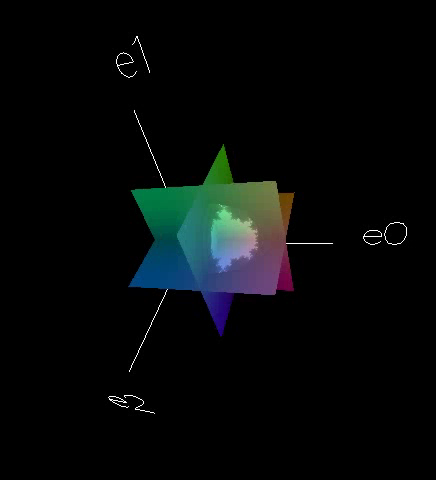
\includegraphics[width=0.4\textwidth]{3dmandel1}
 & 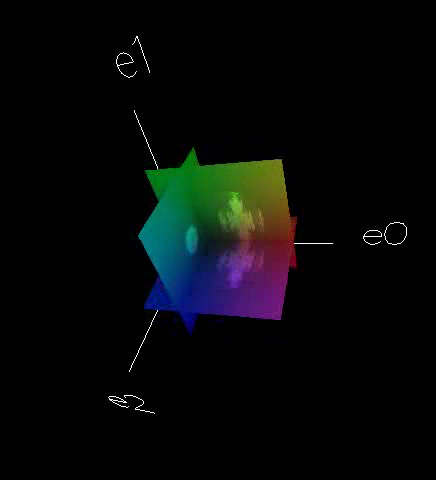
\includegraphics[width=0.4\textwidth]{3dmandel2} 
\end{tabular}
\caption{\label{fig:3dmandel}
  Two frames from an animation\cite{FRAC:MandelAnim} showing slices through
          the 3 dimensional Mandelbrot set.}
\end{figure}

FIXME: ... voxel stuff

%Since we are no longer restricted to the complex plane we may choose many ways
%to associate an image plane point $(x,y)$ with a corresponding constant
%vector $c$. 

In figure \ref{fig:3dmandel} vectors lying in three orthogonal
planes were used to generate three images of the three-dimensional
Mandelbrot set which are then displayed mapped onto the original planes. This
gives a crude visualisation method. A better method used to generate pictures
of the generalised Julia set is given below.

\subsection{The Generalised Julia Set}

\begin{figure}
\centering
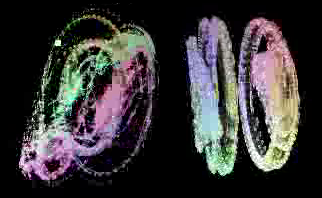
\includegraphics[width=0.8\textwidth]{3djulia_pair}
\caption{\label{fig:3djulia}
  Two frames from an animation\cite{FRAC:JuliaAnimation} showing voxel
          rendering of 3d Julia sets.}
\end{figure}

We may generalise the Julia set in an analogous manner and generate it
using algorithm \ref{alg:generalised_julia}.

\begin{definition}[The generalised Julia set]
The generalised Julia set, $\mathbb{J}_{c,k}$, in $\mathbb{R}^k$
which is associated with the vector $c \in \mathbb{R}^k$ is given by
\[
\mathbb{J}_{c,k} = 
\left\{x \in \mathbb{R}^k
: \lim_{n \rightarrow \infty} f_v^{(n)}(x) < \infty \right\}.
\]
\end{definition}

\begin{fancyalg}
\begin{algorithmic}[1]
\REQUIRE{Set $\mathcal I$ of vectors associated with image points}
\REQUIRE{$c =$ constant vector}
\STATE $i_{\mathrm{max}} :=$ maximum number of iterations
\STATE $e_1 :=$ a unit vector in some preferred direction
\FORALL{$r \in {\mathcal I}$}
\STATE $i := 0$
\WHILE{$r^2 < 4$ and $i < i_{\mathrm{max}}$}
  \STATE $r := re_1r + c$
  \STATE $i := i+1$
\ENDWHILE 
\STATE set pixel $r$ to colour $i$
\ENDFOR
\end{algorithmic}
\caption{
\label{alg:generalised_julia}
  Generating the Generalised Julia set}
\end{fancyalg}

\begin{figure}
\centering
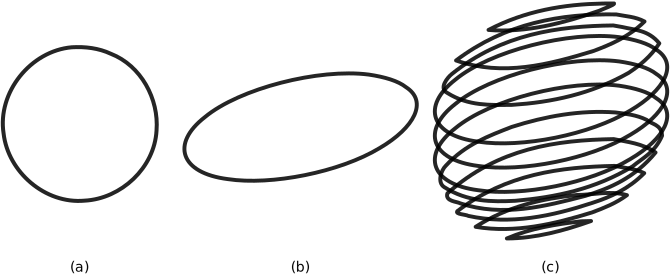
\includegraphics[width=0.8\textwidth]{voxel}
\caption{\label{fig:voxel}
  A crude form of voxel rendering. (a) A specific slice through the set. (b) Viewed from
  an oblique angle. (c) Stacked with other slices giving the impression of a three
  dimensional shape.
}
\end{figure}

Figure \ref{fig:3djulia} was rendered using a crude form of voxel rendering. A
number of 2-dimensional 'slices' were rendered at varying heights in the set. Each
pixel was coloured, or left transparent, depending on whether it was within or without
the set. Finally, each slice was rendered at an oblique angle. The resulting
`stack' of slices gave an approximation to the true shape. Figure
\ref{fig:voxel} illustrates this process.

The voxel rendering was adequate to visualise the fractals and confirm the algorithm
works, but a more sophisticated rendering technique is desirable which can generate
sharper images.

\subsection{Ray Tracing}

In this section we briefly extend the method in \cite{FRAC:HypercomplexIterations} of 
ray-tracing quaternionic escape-time fractals to the generalised GA fractals developed 
above. Ray-tracing of fractals is acheived by finding some distance function
$d(x;\Omega)$ which gives the minimum distance to the fractal parameterised by
$\Omega$ along the from the point $x$. For a Julia fractal the
parameter $\Omega$ is the constant $c$. For a Mandelbrot fractal there is no
paramter as the fractal is unique. 

In \cite{FRAC:HypercomplexIterations} it was shown, for the complex number
form of the escape time fractals above, that such a distance function
at a point $z$ in the complex plane $d_z$ was bounded by
\[
d_z > \lim_{n \arrow \infty}\,\frac{|z_n|}a{2|z'_n|}\log|z_n|
\]
where $z_n = z_{n-1}^2 + c$, $|z'_n| = 2|z_{n+1}||z'_{n+1}|$, $z'_0 = 0$.
The values of $z_0$ and $c$ were dictated by the type of fractal as described above.

It was found that extending the formula to vectors using our analogue of
complex multiplication yielded a suitable distance function although this has not
yet been formally proved. Specifically
\[
d(x; \Omega) = \lim_{n \arrow \infty}\,\frac{|x_n|}a{2|x'_n|}\log|x_n|
\]
where $x_n = f_v(x_{n-1})$, $|x'_n| = 2|x_{n+1}||x'_{n+1}|$, $x'_0 = 0$ and
the initial value of $x_n$ is fractal dependant. 

Once a distance function (or a lowerebound thereof) is available ray tracing
becomes possible. Rays of light are traced back from point in the image
plane of an imaginary camera to the scene. For a particular ray the algorithm
to trace the fractal is as follows.

\begin{enumarate}
\item Set $\hat{r}$ to be a unit vector pointing along the ray direction.
\item Set the current position, $x$, to be the camera origin.
\item Calculate a lower bound, $d_-$ for the distance from $x$. 
\item If $d_-$ is smaller than some tolerance $\tau$ exit reporting
$x$ as the intersection point with the fractal.
\item Set $x \leftarrow x + d_-\hat{r}$.
\item Go to step 3.
\end{enumerate}

\begin{figure}
\centering
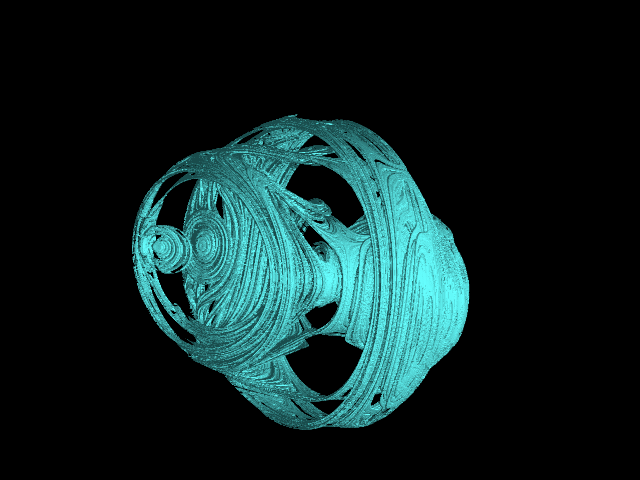
\includegraphics[width=0.8\textwidth]{5djulia}
\caption{\label{fig:5djulia}
  A ray-traced three-dimensional slice through a five-dimensional Julia set.
}
\end{figure}

Once the intersection point is found the fractal may be lit by examining
intersection points of neighbouring rays and taking the surface orientation
to be that of a plane passing through the neighbouring intersection points.
Figure \ref{fig:5djulia} shows a slice through a 5d Julia set rendered with
this technique.

\section{Moving to Hyperbolic Geometry}

So far all our fractals have been generated using the Euclidean geometry of
the complex plane or $n$-dimensional flat space. In this section we
extend our algorithm using the non-Euclidean tools
given to us by conformal GA. We firstly need to re-define our complex function
in terms of the geometric operations.

Viewed using Euclidean geometry our function $f(r)$ firstly reflects and
scales the vector $r \mapsto re_1r$ and then translates via the vector $c$. We
know already how to translate using conformal GA so we turn our attention to
the former operation.

Since we constructed our GA approach to be analogous to the complex number approach we
may borrow the geometric interpretation from complex numbers. In this case the mapping 
$r \mapsto r^2$ acts to rotate r by $\mathrm{arg}(r)$ and scale it by
$\magof{r}$. We may therefore extend this interpretation into our GA solution as in
figure \ref{fig:rotate}. We firstly work only in the $r \wedge e_1$ plane to allow
our analogy with complex numbers to hold. If $\theta$ is the angle between $r$ and
$e_1$, i.e.
\[
\theta = \cos^{-1}\left(\frac{r \cdot e_1}{\magof{r}}\right),
\] 
then the mapping $r \mapsto re_1r$ is initially a rotation in the plane $r \wedge e_1$
by $\theta$ followed by a dilation by a factor of $(r^2)^\frac{1}{2}$ 
which may be expressed in terms of rotors and dilators using their geometric
definitions above.

\begin{definition}
The conformal GA analogue of $r \mapsto re_1r$ is given by
\[
F(re_1r) = D_r R_r\,F(r)\,\tilde{R}_r \tilde{D}_r
\]
where
\begin{eqnarray*}
R_r & = & \cos \frac{\theta}{2} + P \sin \frac{\theta}{2},
    \quad
P = \frac{(r \wedge e_1)}{\magof{r}}
\end{eqnarray*}
and $\theta$ is defined above.
The dilator $D_r$ acts to dilate about the origin by a factor of
$\magof{r}$. In Euclidean geometry it is given by
\[
D_r = \exp\left( \frac{-\log(\magof{r})}{2} e\bar{e} \right).
\]
\end{definition}

\begin{figure}
\centering
\includegraphics[width=0.5\textwidth]{rotate}
\caption{\label{fig:rotate}%
  The geometrical interpretation of $r \mapsto re_1r$ as a rotation followed by a dilation.
}
\end{figure}

The second part of $f(r)$ is a translation by $c$. A translator in non-Euclidean
geometries is only defined as translating the origin to a given point so we must be
careful about the precise operations we perform. The GA analogue of the
complex mapping $r \mapsto r + c$ is thus given by the following steps:
\begin{enumerate}
\item Translate $r$ to the origin by applying the appropriate geometry-specific translator represented by $\tau(-r)$;
\item Translate the origin to $c$ by applying the translator $\tau(c)$;
\item `Undo' step 1 by applying the translator $\tau(r)$.
\end{enumerate}
where $\tau(r)$ is a function which will give the appropriate translator for our 
chosen geometry. In Euclidean geometry $\tau(r) = 1 + \frac{nr}{2}$ and in
non-Euclidean geometry
\[
\tau(r) = \frac{1}{\sqrt{\lambda^2 - r^2}}(\lambda + \bar{e}r)
\]
with $\lambda$ being defined as in the discussion of non-Euclidean geometries above.

A little thought will reveal that this is equivalent to translating $c$ by the translator
$1 + \frac{nr}{2}$. We may therefore define our full conformal GA analogue of $f(r)$.

\begin{definition}
The conformal GA analogue of $f(r) = re_1r + c$ is given by
\[
f(r) = F^{-1}(T_r F(c) \tilde{T}_r)
\]
where
\[
T_r = \tau(F^{-1}(D_r R_r\,F(r)\,\tilde{R}_r \tilde{D}_r))
\]
\end{definition}

\begin{figure}[p]
\centering
\begin{tabular}{c}
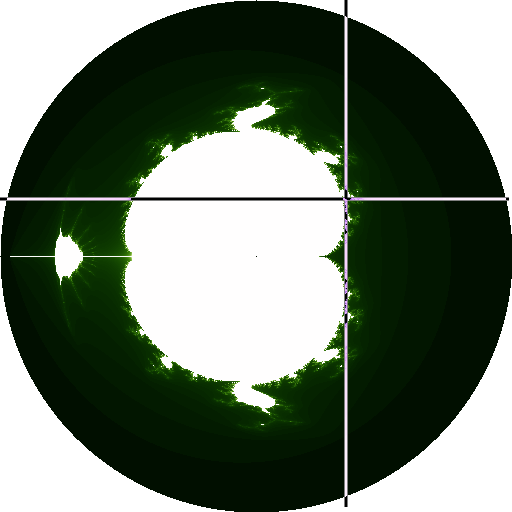
\includegraphics[width=0.35\textheight]{hyp_mandel_julia_pos} \\ (a) \\
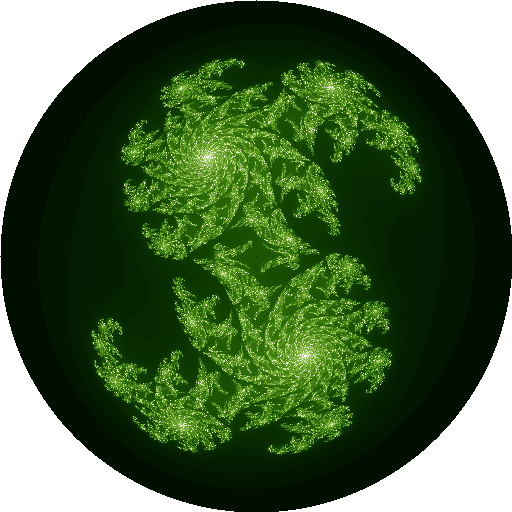
\includegraphics[width=0.35\textheight]{julia_hyp} \\
                          (b)
\end{tabular}
\caption{\label{fig:noneuclidean_sets}The non-Euclidean analogue of the (a) Mandelbrot set with
  the constant $c = 0.4e_1 + 0.2e_2$ marked and (b) the Julia
  set associated with $c$.}
\end{figure}

Our algorithm for generating the generalised Mandelbrot and Julia sets is now identical
except we substitute our new, geometric, definition of $f(r)$ and choose $\tau(r)$
and the form of $D_r$ to reflect our chosen geometry. Usefully pure-rotation rotors remain
the same in each geometry so no modification of them is necessary. Figure
\ref{fig:noneuclidean_sets} shows a hyperbolic Mandelbrot and Julia set on the
Poincar\'e disc generated with this method. 

\subsection{The Hyperbolic Mandelbrot Set}

The hyperbolic Mandelbrot set is shown in figure \ref{fig:noneuclidean_sets}a and
is generated using algorithm \ref{alg:generalised_mandelbrot}, substituting
step 7 for one performing the iteration outlined above. 

\subsection{The Hyperbolic Julia Set}

A particular hyperbolic Julia set is shown in figures \ref{fig:noneuclidean_sets}b
and \ref{fig:julia_montage}.  Once again, it is generated using algorithm
\ref{alg:generalised_julia} substituting step 6.

\begin{figure}[p]
\centering
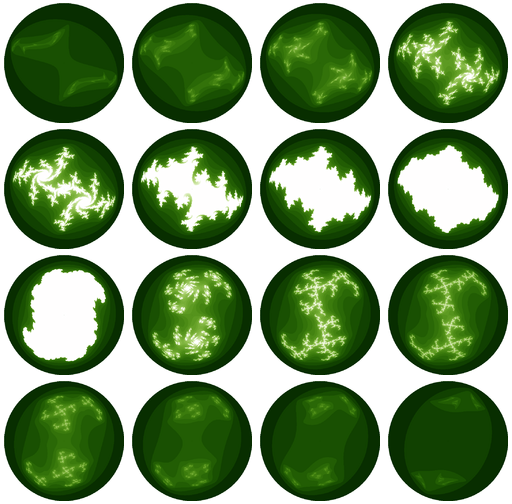
\includegraphics[width=0.9\textwidth]{julia_montage}
\caption{\label{fig:julia_montage} 
  A montage of hyperbolic Julia sets where the constant $c$ moves from $-0.7e_1 - 0.7e_2$
  to $0.7e_1 + 0.7e_2$. 
  In this figure translation $x \mapsto x + c$ is performed by applying a
  translation rotor corresponding to $c$ to the vector $x$.
}
\end{figure}

\begin{figure}[p]
\centering
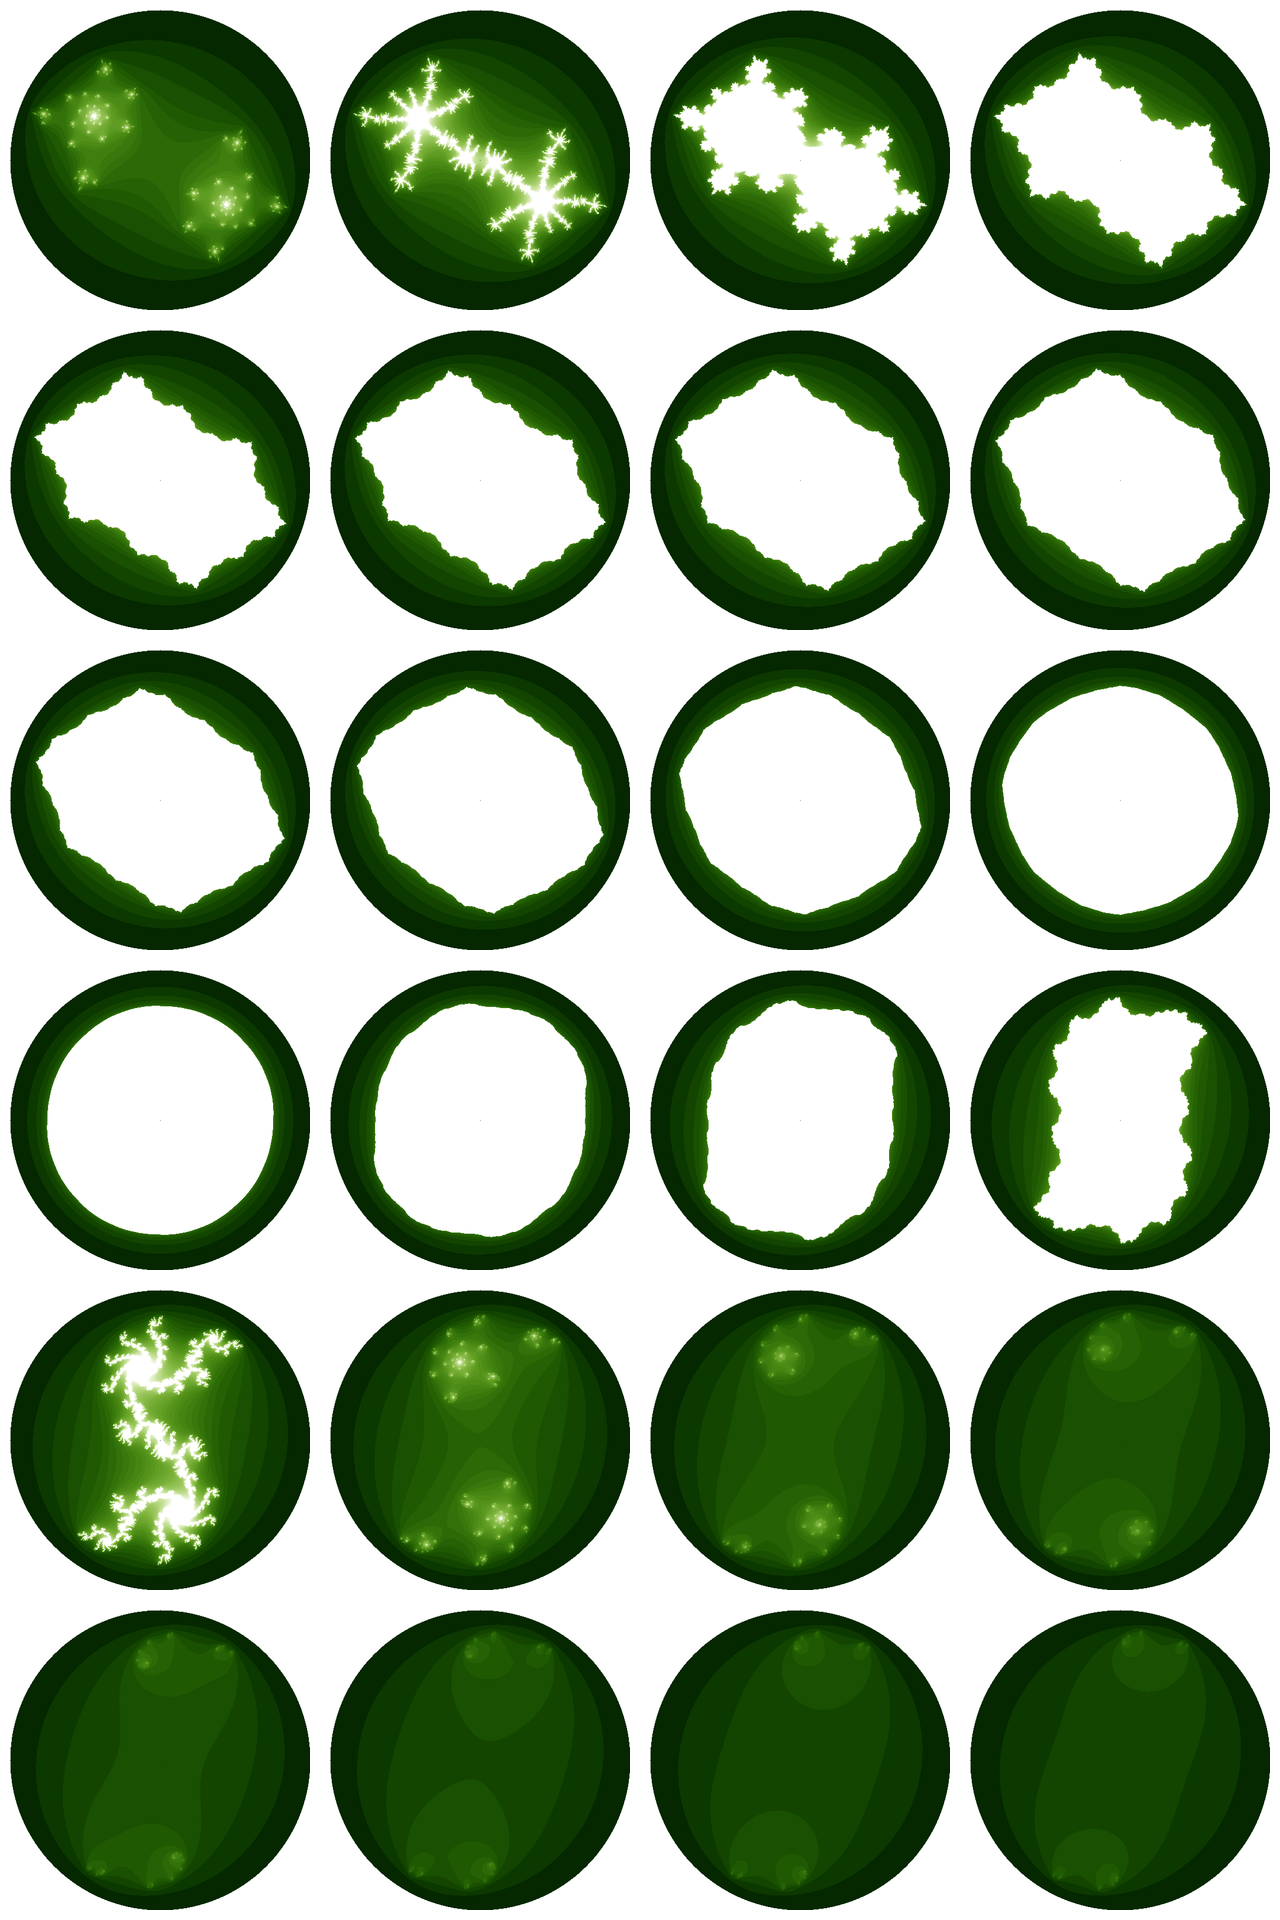
\includegraphics[width=0.9\textwidth]{direct_julia_noneuclid}
\caption{\label{fig:direct_julia_noneuclid} 
  A montage of hyperbolic Julia sets where the constant $c$ moves from $-0.7e_1 - 0.7e_2$
  to $0.7e_1 + 0.7e_2$. 
  In this figure translation $x \mapsto x + c$ is performed by applying a
  translation rotor corresponding to $x$ to the vector $c$.
}
\end{figure}

It is worth noting that the code to generate the Euclidean fractals in figure 
\ref{fig:euclidean_sets} is identical to that used to generate
\ref{fig:julia_montage} except for the definition of translators and dilators.
We can replace the Euclidean form with those given in section
\ref{sec:extendconfmodel} and re-cast the fractals into hyperbolic geometry.
The fact that conformal GA algorithms developed using Euclidean geometry may
so readily be applied to non-Euclidean geometries by simply changing the rotor
definitions neatly indicates the power of the conformal GA approach.




\begin{savequote}
\quoteperson{There is no branch of mathematics, however abstract, which may
  not someday be applied to the phenomena of the real world.}%
{Nicolai Lobachevsky}%
\end{savequote}

\chapter{Rotors as Exponentiated Bivectors}

In this chapter we shall consider common representations for pure-rotation
rotors, translators and combinations of the both. We shall term rotors which
represent rotations and translations \emph{general displacement} rotors. We
will not explicitly deal with other rotors, such as dilation rotors, but
similar techniques may be useful for their investigation.  If we examine the
form of the rotors presented in chapter \ref{chap:introduction} we see that
all of them have a common form; they are all exponentiated bivectors.
Rotations are generated by exponentiating bivectors with no
$e$ or $\bar{e}$-like components in them. We term objects with no contribution
from $e$ and $\bar{e}$ \emph{spatial}.
We may
postulate that all general displacement rotors can be expressed as
\[
R = \exp(B)
\]
where $B$ is the sum of two bivectors, one spatial and
the other formed from the outer product of
$n$ with a spatial vector. Our justification being that those closely match
the form of the bivectors which generate rotation and translation rotors 
respectively. The effect of this is to separate the basis bivectors of $B$
into one with components of the form $e_i \wedge e_j$ and one with components
of the form $e_i \wedge e$ and $e_i \wedge \bar{e}$.

Notationally, we assume all general displacement rotors can be formed by
exponentiating a bivector of the form $B = ab + cn$ where $a$, $b$ and $c$ are
independent of $n$, i.e. if $n \in \mathcal{A}(m+1,1)$ then $\{a,b,c\} \in
\mathbb{R}^m$.  It is clear that the set of all $B$ is some linear sub-space
of all the bivectors.

We now suppose that we may interpolate rotors by defining some function
$\ell(R)$ which acts upon rotors to give the generating bivector element. We
then perform direct interpolation of these generators.  We postulate that
direct interpolation of these bivectors, as in the reformulation of
quaternionic interpolation in section \ref{sec:quaternions}, will give some
smooth interpolation between the displacements.  It is therefore a defining
property of $\ell(R)$ that
\begin{equation}
R \equiv \exp(\ell(R))
\end{equation}
and so $\ell(R)$ may be considered as to act as a logarithm-like function in
this context.  It is worth noting that $\ell(R)$ does not possess all the
properties usually associated with logarithms, notably that, since
$\exp(A)\exp(B)$ is not generally equal to $\exp(B)\exp(A)$ in non-commuting
algebras, $\ell(\exp(A)\exp(B))$ cannot be equal to $A + B$ except in special
cases.

To avoid the the risk of assigning more properties to $\ell(R)$ than we have
shown, we shall resist the temptation to denote the function $\log(R)$. The
most obvious property of $\log(\cdot)$ that $\ell(\cdot)$ doesn't possess is
$\log(AB) = \log(A) + \log(B)$. This is clear since the geometric product is
not commutative in general whereas addition is.

\section{Form of $\exp(B)$ in Euclidean space}
\label{subsec:form}

\begin{definition}[Spatial elements]
An element $x$ in the conformal model is termed `spatial' if
\[
x \cdot e = x \cdot \bar{e} = 0.
\]
\end{definition}

\begin{lemma}
\label{lem:bk}
If $B$ is of the form $B=\phi P+tn$ where 
$t$ is a spatial vector, $\phi$ is some scalar and $P$ is a spatial bivector
where $P^2 = -1$ then, for any $k \in \mathbb{Z}^+$, 
\[
B^{k}=\phi^k P^{k}+\alpha _{k}^{(1)}\phi Ptn+
\alpha _{k}^{(2)}\phi^2 PtnP+\alpha _{k}^{(3)}\phi tnP+\alpha _{k}^{(4)}tn
\]
with the following recurrence relations for $\alpha _{k}^{(\cdot )}$,
$k>0$ 

\begin{centering}

\begin{tabular}{r@{$\ =\ $}lr@{$\ =\ $}l}
$\alpha _{k}^{(1)}$ & $- \phi^2 \alpha _{k-1}^{(2)}$ &
$\alpha _{k}^{(2)}$ & $\alpha _{k-1}^{(1)}$\\
$\alpha _{k}^{(3)}$ & $\alpha _{k-1}^{(4)}$ &
$\alpha _{k}^{(4)}$ & $\phi^{k-1}P^{k-1} - \phi^2 \alpha_{k-1}^{(3)}$
\end{tabular}

\end{centering}

\noindent with 
$\alpha _{0}^{(1)}=\alpha _{0}^{(2)}=
\alpha _{0}^{(3)}=\alpha _{0}^{(4)}=0$.
\end{lemma}
\begin{proof}
Firstly note that the theorem is trivially provable by direct 
substitution for the cases $k=0$ and $k=1$. We thereafter seek a 
proof by induction.

Assuming the expression for $B^{k-1}$ is correct, we post-multiply
by $\phi P+tn$ to obtain
\begin{eqnarray*}
B^k & = & \phi^k P^k + \alpha_{k-1}^{(1)}\phi^2 PtnP + 
          \alpha_{k-1}^{(2)}\phi^3 PtnP^2 + \alpha_{k-1}^{(3)}\phi^2 tnP^2 + \\
    &   & \alpha_{k-1}^{(4)}\phi tnP + \phi^{k-1} P^{k-1} tn + \alpha_{k-1}^{(1)}\phi P(tn)^2 +
          \alpha_{k-1}^{(2)}\phi^2 PtnPtn + \\
    &   & \alpha_{k-1}^{(3)}\phi tnPtn +
	  \alpha_{k-1}^{(4)}(tn)^2
\end{eqnarray*}

Substituting $P^2 = -1$, $(tn)^2 = - tn^2t = 0$ and noting that
$nPt = - Ptn$ leading to $tnPtn = - tPtn^2 = 0$

\begin{eqnarray*}
B^k & = & \phi^k P^k + \alpha_{k-1}^{(1)}\phi^2 PtnP -
          \alpha_{k-1}^{(2)}\phi^3 Ptn - \alpha_{k-1}^{(3)}\phi^2 tn + \\
    &   & \alpha_{k-1}^{(4)}\phi tnP + \phi^{k-1} P^{k-1} tn \\
    & = & \phi^k P^k - (\alpha_{k-1}^{(2)}\phi^2)\phi Ptn +
          \alpha_{k-1}^{(1)}\phi^2 PtnP + \\
    &   & \alpha_{k-1}^{(4)}\phi tnP +
	  (\phi^{k-1} P^{k-1}  - \alpha_{k-1}^{(3)}\phi^2) tn
\end{eqnarray*}

Equating like coefficients we obtain the required recurrence relations.
\end{proof}

\begin{lemma}
\label{lem:bkexp}
Assuming the form of $B$ given in lemma \ref{lem:bk}, for 
$k\in \mathbb{Z}^{+}$,\[
B^{2k}=(-1)^k\phi^{2k}-k(-1)^k\phi^{2k-1}[tnP + Ptn]
\]and\[
B^{2k+1}=(-1)^k\phi^{2k+1}P + k \phi^{2k} (-1)^k [ tn - PtnP ] + (-1)^k\phi^{2k} tn
\]
\end{lemma}
\begin{proof}
Starting from $\alpha _{0}^{(.)}=0$ it is clear that the recurrence
relations above imply that $\alpha _{k}^{(1)}=\alpha _{k}^{(2)}=0\; \forall \: k \ge 0$.
Substituting $\alpha _{k}^{(3)}=\alpha _{k-1}^{(4)}$ it is trivial to show
that the relation for $\alpha _{k}^{(4)}$ is satisfied by \[
\alpha _{k}^{(4)}=\begin{cases}
 \frac{k}{2}(\phi P)^{k-1} & k\textrm{ even,}\\
 \frac{k+1}{2}(\phi P)^{k-1} & k\textrm{ odd.}\end{cases}\]
When substituted into the expression for $B^{k}$, we obtain the
result stated above.
\end{proof}

\begin{thm}
\label{lem:exp}
If $B$ is a bivector of the form given in lemma \ref{lem:bk}
then, defining 
$t_\parallel$ as the component of $t$ lying in the plane of $P$ 
and $t_\perp = t - t_\parallel$,
\[
\exp(B) = \left[ \cos(\phi) + \sin(\phi) P \right] \left[ 1 + t_\perp n \right] + \sinc(\phi) t_\parallel n
\]
\end{thm}
\begin{proof}
Consider the power series expansion of $\exp (B)$,
\[
\exp (B)=\sum _{k=0}^{\infty }\frac{B^{k}}{k!}=\sum _{k=0}^{\infty }\left[\frac{B^{2k}}{(2k)!}+\frac{B^{2k+1}}{(2k+1)!}\right]\]
Substituting the expansion for $B^{2k}$ and $B^{2k+1}$ from 
lemma \ref{lem:bkexp}
\begin{align*}
\exp (B)= & \sum _{k=0}^{\infty }\left[
 \frac{
   (-1)^k\phi^{2k}
 }{(2k)!} - k \frac{
   (-1)^k\phi^{2k-1}
 }{(2k)!} \left(tnP + Ptn\right)
\right]\\
+ & \sum _{k=0}^{\infty }\left[
 \frac{
   (-1)^k\phi^{2k}
 }{(2k+1)!} \left(\phi P + tn\right) + 
 k\frac{
   (-1)^k \phi^{2k}
 }{(2k+1)!} \left( tn - PtnP \right)\right]
\end{align*}
We now substitute the following power-series representations

\begin{centering}

%\[
%\begin{array}{r@{=}l@{\quad}r@{=}l}
%\cos(z) & \sum_{k=0}^\infty \frac{(-1)^k z^{2k}}{(2k)!} &
%\sinc(z) & \sum_{k=0}^\infty \frac{(-1)^k z^{2k}}{(2k+1)!} \\
%- z \sin(z) & \sum_{k=0}^\infty 2k \frac{(-1)^k z^{2k}}{(2k)!} &
%\cos(z) - \sinc(z) & \sum_{k=0}^\infty 2k \frac{(-1)^k z^{2k}}{(2k+1)!}
%\end{array}
%\]

\begin{tabular}{r@{$\ =\ $}l@{$\quad$}r@{$\ = \ $}l}
\multicolumn{4}{l}{\vspace{0.1cm}} \\
$\cos(z)$ & $\sum_{k=0}^\infty \frac{(-1)^k z^{2k}}{(2k)!}$ &
$\sinc(z)$ & $\sum_{k=0}^\infty \frac{(-1)^k z^{2k}}{(2k+1)!}$ \\
\multicolumn{4}{l}{\vspace{0.1cm}} \\
$- z \sin(z)$ & $\sum_{k=0}^\infty 2k \frac{(-1)^k z^{2k}}{(2k)!}$ &
$\cos(z) - \sinc(z)$ & $\sum_{k=0}^\infty 2k \frac{(-1)^k z^{2k}}{(2k+1)!}$ \\
\multicolumn{4}{l}{\vspace{0.1cm}} \\
\end{tabular}

\end{centering}

\noindent to obtain
\begin{align*}
\exp(B) = & 
  \cos \phi + \sin(\phi) \frac{1}{2} (tnP + Ptn) + \sinc(\phi) (\phi P + tn) \\
+ & \frac{1}{2} \left[ \cos(\phi) - \sinc(\phi) \right] (tn - PtnP)
\end{align*}
By considering parallel and perpendicular components of $t$ with
respect to the plane of $P$ we can verify that
$tnP + Ptn = 2 Pt_\perp n$ and $PtnP = (t_\parallel - t_\perp)n$ hence
\begin{align*}
\exp(B) = & 
  \cos \phi + \sin(\phi) P t_\perp n + \sinc(\phi) (\phi P + tn) + \left[ \cos(\phi) - \sinc(\phi) \right] t_\perp n \\
  = & \cos (\phi) \left[ 1 + t_\perp n \right] +
  \sin(\phi) P \left[ 1 + t_\perp n \right] + \sinc(\phi) t_\parallel n \\
  = & \left[ \cos(\phi) + \sin(\phi) P \right] \left[ 1 + t_\perp n \right] + \sinc(\phi) t_\parallel n 
\end{align*}
as required.
\end{proof}

\begin{definition}
A \emph{twist} is a rotor whose action is to rotate by $\phi$ in the 
plane of $P$ whilst translating along a vector $a$ perpendicular to
the plane of $P$. It may therefore be 
defined by the rotor 
\[
\tau(\phi, P, a) =
 \left[ \cos\left(\frac{\phi}{2}\right) +
   \sin\left(\frac{\phi}{2}\right)P
 \right]
 \left[
   1 + \frac{na}{2}
 \right]
\]
where $\phi$ is a scalar, $P$ is a spatial bivector normalised such that 
$P^2 = -1$ and $a$ is some vector satisfying $a \cdot n = a \cdot P = 0$.
\end{definition}

\begin{lemma}
The exponentiation function may be re-expressed using a twist
\[
\exp\left(\frac{\phi}{2}P + \frac{tn}{2}\right) =
\left[ 1 + \sinc\left(\frac{\phi}{2}\right)\frac{t_\parallel n}{2} \tilde{\tau}(\phi, P, - t_\perp) \right]
\tau(\phi, P, - t_\perp)
\]
\end{lemma}
\begin{proof}
We firstly substitute our definition of a twist into our form for the exponential
\begin{equation}
\exp\left(\frac{\phi}{2}P + \frac{tn}{2}\right) =
\tau(\phi, P, - t_\perp) + \sinc\left(\frac{\phi}{2}\right)\frac{t_\parallel n}{2}
\label{eqn:twistform}
\end{equation}
noting that, since twists are rotors, $\tau( \cdot ) \tilde{\tau}(\cdot) = 1$, it is
then clear that the required expression is equivalent to this form of the exponential.
\end{proof}

\begin{lemma}
The expression
\[
 1 + \sinc\left(\frac{\phi}{2}\right)\frac{t_\parallel n}{2} \tilde{\tau}(\phi, P, - t_\perp)
\]
is a rotor which acts to translate along a vector $t'_\parallel$ given by
\[
t'_\parallel = - \sinc\left(\frac{\phi}{2}\right)
t_\parallel
\left(
\cos\left(\frac{\phi}{2}\right) -
\sin\left(\frac{\phi}{2}\right) P 
\right)
\]
\end{lemma}
\begin{proof}
The expression above may be obtained by substituting for the twist in the initial expression and simplifying. 
It is clearly a vector since multiplying $t_\parallel$ on the left by $P$ is just a rotation by $\pi / 2$ in the plane
of $P$.
\end{proof}

We have now developed the required theories and tools to discuss the
action of the rotor
\[
R = \exp\left(
\frac{\phi}{2} P + \frac{tn}{2}
\right)
\]
It translates along a vector $t_\perp$ which is the component of $t$ which does not lie in the
plane of $P$, rotates by $\phi$ in the plane of $P$ and finally translates along 
$t'_\parallel$ which is given by
\[
t'_\parallel =- \sinc\left(\frac{\phi}{2}\right)
t_\parallel
\left(
\cos\left(\frac{\phi}{2}\right) -
\sin\left(\frac{\phi}{2}\right) P 
\right)
\]
which is the component of $t$ lying in the
plane of $P$, rotated by $\phi/2$ in that plane.

\section{Checking $\exp(B)$ is a rotor}

It is sufficient to check that $\exp(B)$ satisfies the following
properties of a rotor $R$. % in Euclidean space
\[
R\tilde{R} = 1, \quad Rn\tilde{R} = n
\]

\begin{thm} If $R = \exp(B)$ and $B$ is a bivector of the form 
given in lemma
\ref{lem:bk} then $R\tilde{R} = 1$.
\end{thm}
\begin{proof}
Consider the twist form of $\exp(B)$ from equation \ref{eqn:twistform}
\[
R = \exp(B) =
\tau(\phi, P, - t_\perp) + \sinc\left(\frac{\phi}{2}\right)\frac{t_\parallel n}{2}
\]
and make use of our knowledge that $\tau(\phi, P, - t_\perp)$ is a rotor.
Hence,
\begin{eqnarray*}
R\tilde{R} & = & \tau(\phi, P, - t_\perp)\tilde{\tau}(\phi, P, - t_\perp)
+ \sinc^2\left(\frac{\phi}{2}\right)
\frac{t_\parallel n^2 t_\parallel}{4}\\
&& + \ \sinc\left(\frac{\phi}{2}\right)
\left[ \tau(\phi, P, - t_\perp)nt_\parallel + 
       t_\parallel n\tilde{\tau}(\phi, P, - t_\perp) \right] \\
& = & 1 + 0 + \sinc\left(\frac{\phi}{2}\right)
\left[ T + \tilde{T} \right]
\end{eqnarray*}
where $T = \tau(\phi, P, - t_\perp)nt_\parallel$.

Looking at the definition of $\tau(\phi, P, - t_\perp)$, it is clear
that it has only scalar, bivector and 4-vector components with
the bivector components being parallel to $P$ or $t_\perp n$ and
the 4-vector components being parallel to $Pt_\perp n$. When
post-multiplied by $nt_\parallel$ to form $T$, the 4-vector component
goes to zero (since $n^2 = 0$) as does the bivector component
parallel to $t_\perp n$ and so we are left with $T$ having only
components parallel to $nt_\parallel$ and $Pnt_\parallel$. 
We may now express $T$ as
\[
T = \alpha nt_\parallel + \beta Pnt_\parallel
\]
where $\alpha$ and $\beta$ are suitably valued scalars. Hence
\[
T + \tilde{T} = \alpha \left[ nt_\parallel + t_\parallel n \right]
+ \beta \left[ Pnt_\parallel + t_\parallel n\tilde{P} \right] 
= 0 + \beta n \left[ Pt_\parallel - t_\parallel \tilde{P} \right]
\]

By considering two basis vectors of $P$, $a$ and $b$, such
that $P = ab$, $a \cdot b = 0$ and resolving $t_\parallel$ in 
terms of $a$ and $b$ it is easy to show that 
$Pt_\parallel - t_\parallel\tilde{P} = 0$ and hence
$T + \tilde{T} = 0$ giving the required result.
\end{proof}

\begin{thm} If $R = \exp(B)$ and $B$ is a bivector of the form 
given in lemma
\ref{lem:bk} then $Rn\tilde{R} = n$.
\end{thm}
\begin{proof}
Again using the twist form of $R$ from equation \ref{eqn:twistform} we have
\begin{eqnarray*}
Rn & = & \tau(\phi, P, - t_\perp)n + 
\sinc\left(\frac{\phi}{2}\right)\frac{t_\parallel n^2}{2} \\
&=& \tau(\phi, P, - t_\perp)n + 0
\end{eqnarray*}
Defining the rotation rotor $R_{(P,\phi)}$ as
\[
R_{(P,\phi)} = \cos\left(\frac{\phi}{2}\right) +
   \sin\left(\frac{\phi}{2}\right)P
\]
and substituting for the definition of the twist above gives
\[
Rn = R_{(P,\phi)} n
\]
Similarly, again using the twist form of $R$ we have
\begin{eqnarray*}
nR & = & n\tau(\phi, P, - t_\perp) + 
\sinc\left(\frac{\phi}{2}\right)\frac{nt_\parallel n}{2} \\
% & = & n\tau(\phi, P, t_\perp) - 
%\sinc\left(\frac{\phi}{2}\right)\frac{t_\parallel n^2}{2} \\
&=& n\tau(\phi, P, - t_\perp) + 0 \\
&=& n R_{(P,\phi)} \left( 1 + \frac{tn}{2} \right) \\
&=& R_{(P,\phi)} n \left( 1 + \frac{tn}{2} \right) \\
&=& R_{(P,\phi)} n 
\end{eqnarray*}
We now have that $Rn = nR$ and hence, using
$R\tilde{R} = 1$ from the previous thm, 
$Rn\tilde{R} = nR\tilde{R} = n$.
\end{proof}

\section{Method for evaluating $\ell(R)$}

We have found a form for $\exp(B)$ given that $B$ is in a particular form.
Now we seek a method to take an arbitrary displacement
rotor, $R = \exp(B)$ and re-construct the original $B$. Should there exist
a $B$ for all possible $R$, we will show that our initial assumption
that all displacement rotors can be formed from a single exponentiated bivector
of special form is valid. We shall term this initial bivector
the \emph{generator} rotor (to draw a parallel with Lie algebras).

We can obtain the following identities for $B=(\phi / 2) P + tn / 2$ by simply considering
the grade of each component of the exponential:
\begin{eqnarray*}
\left< R \right>_0 & = & \cos\left(\frac{\phi}{2}\right) \\
\left< R \right>_2 & = & \sin\left(\frac{\phi}{2}\right) P + 
  \cos\left(\frac{\phi}{2}\right) t_\perp n + \sinc\left(\frac{\phi}{2}\right) t_\parallel n \\
\left< R \right>_4 & = & \sin\left(\frac{\phi}{2}\right) Pt_\perp n
\end{eqnarray*}

It straight forward to reconstruct $\phi, t_\perp$ and
$t_\parallel$ from these components by partitioning a rotor as above. Once we
have a method which gives the generator $B$ for any displacement rotor $R$ we
have validated our assumption.

\begin{thm}
The inverse-exponential function $\ell(R)$ is given by
\[
\ell(R) = ab + \cperp n + \cpar n
\]
where
\begin{eqnarray*}
\magof{ab} & = & \sqrt{\left| (ab)^2 \right|}  = \cos^{-1}(\left<R\right>_0) \\
ab & = & \frac{\left(\left<R\right>_2 n \right) \cdot e}
{\sinc\left(\magof{ab}\right)}\\
\cperp n & = & - \frac{ab \left<R\right>_4}
{\magof{ab}^2\sinc(\magof{ab})} \\
\cpar n & = & - \frac{ab \left<ab \left<R\right>_2\right>_2}
{\magof{ab}^2\sinc(\magof{ab})}
\end{eqnarray*}
\end{thm}
\begin{proof}
It is clear from the above that the form of
$\magof{ab}$ is correct. We thus proceed to show the remaining
equations to be true
\begin{eqnarray*}
\left<R\right>_2 & = & \cos(\magof{ab}) \, \cperp n +
\sinc(\magof{ab}) \left[ab + \cpar n\right]\\
\left<R\right>_2 n & = & \sinc(\magof{ab}) \, abn\\
\left(\left<R\right>_2 n\right) \cdot e & = & \sinc(\magof{ab}) \, ab
\end{eqnarray*}
and hence the relation for $ab$ is correct.
\begin{eqnarray*}
\left<R\right>_4 & = & \sinc(\magof{ab}) \, ab\cperp n \\
ab \left<R\right>_4 & = & -\magof{ab}^2 \sinc(\magof{ab}) \, \cperp n 
\end{eqnarray*}
and hence the relation for $\cperp n$ is correct.
\begin{eqnarray*}
\left<R\right>_2 & = & \cos(\magof{ab}) \, \cperp n +
\sinc(\magof{ab}) \left[ab + \cpar n\right]\\
ab \left<R\right>_2 & = & \cos(\magof{ab}) \, ab\cperp n +
\sinc(\magof{ab}) \left[ab \cpar n - \magof{ab}^2\right]\\
\left<ab \left<R\right>_2\right>_2 & = & 
\sinc(\magof{ab}) \, ab \cpar n
\end{eqnarray*}
and hence the relation for $\cpar n$ is correct.
\end{proof}

% \section{Limitations of Current Form}


\section{Mapping Generators to Matrices}

Although the representation of a rotor as an exponentiated generator bivector
is convenient mathematically and useful for smooth pose interpolation
and mesh deformation, as will be presented later, it is somewhat cumbersome
to integrate into an existing graphical pipeline. Most graphics hardware and
nearly all graphics APIs represent rigid-body transformations as $4 \times 4$ matrices.
Specifically given the projective mapping from a three-dimensional vector $\mathbf{x}$ to
its homogeneous representation,
\[
\mathbf{x} \mapsto \left[ \begin{array}{c}
w \mathbf{x} \\ w
\end{array}\right]
\]
where $w$ is some arbitrary non-zero scalar, a rigid body transform can be represented as
\[
 \left[ \begin{array}{c}
w \mathbf{x} \\ w
\end{array}\right]
\mapsto
 \mathcal{R}\left[ \begin{array}{c}
w \mathbf{x} \\ w
\end{array}\right]
\]
and
\[
\mathcal{R} = \left[
\begin{array}{cc}
\mathbf{R} & \mathbf{t} \\
                0 & 1
\end{array}
\right].
\]
Here $\mathbf{R}$ is an orthonormal $3 \times 3$ rotation matrix and $\mathbf{t}$ is some
translation vector.

Due to the common nature of such a representation it would be advantageous to
have some method of mapping between the conveniently linear space of
generators to the decidedly non-linear space of these $4 \times 4$ matrices.
In this section we shall develop such a method. Note that we shall only be
working in three-dimensions due to the limitations of the matrix
representation rather than the exponentiated generator representation.

Recall that we represent a rotor, $R$, as $R = \exp(B)$ where $B$ is a bivector
The generator bivector, $B$, may itself be
parametrised in terms of a spatial bivector $P$ normalised such that
$P^2 = -1$, a scalar $\phi$ and a spacial vector $t$
as in lemma \ref{lem:bk}.
Letting $P = p_1 e_{12} + p_2 e_{23} + p_3 e{31}$ and
$t = t_1 e_1 + t_2 e_2 + t_3 e_3$ we may represent $B$ via the
vector $\mathbf{b}$:
\[
\mathbf{b} = [ p_1 \; p_2 \; p_3 \; t_1 \; t_2 \; t_3 ]^T.
\]

Using this generator representation is useful since any vector
$\mathbf{b} \in {\mathbb R}^6$ will represent a valid generator and
hence a valid rotor.

%the $4\times4$ matrix representation is useful for existing graphics
%algorithms. This note aims to develop an algorithm for converting from
%one to another with the proviso that 

It is also worth noting that this method of converting from a matrix
representation to a generator is lossy in so much as the matrix representation
cannot uniquely represent rotations by more the $2\pi$.

\subsection{Method}

We shall attempt to linearise the application of a rotor associated
with a generator to a point by defining an appropriate linear function
$h(\cdot)$.

\begin{definition}
The function $h(\phi, P, t, p, \lambda)$ is defined, for $\lambda = 1$ as
\[
h(\phi, P, t, p, 1) = F^{-1} \left( R F(p) \tilde{R} \right)
\]
where $R = \exp(B)$, $B = \phi P+tn$ and $P, \phi$ and $t$ are
as defined in lemma \ref{lem:bk}. $F(\cdot)$ is the usual vector 
to null-vector mapping.
\end{definition}

It is easy, if somewhat tedious, to show by direct expansion and comparison of terms that
an expression for $h(\cdot)$ which matches the definition above is
\begin{align}
h(\phi, P, t, p, \lambda) &=c^2p - s^2PpP - sc\left[pP - Pp\right] \nonumber \\
&\quad+ \lambda\left[ 
 \frac{kc+1}{2} t + \frac{kc-1}{2} PtP
- \frac{sk}{2} (tP - Pt)
\right] \label{eqn:defnh}
\end{align}
where $s = \sin(\phi/2)$, $c = \cos(\phi/2)$ and $k = \textrm{sinc}(\phi/2)$.

\begin{definition}
The function $\mathbf{v}(x)$ maps the $m$-dimensional vector $x$ to its column-vector
representation,
\[
\mathbf{v}(x) = \left[
\begin{array}{c}
x \cdot e_1 \\ x \cdot e_2 \\ \vdots \\ x \cdot e_m
\end{array} 
\right].
\]
\end{definition}

It is clear by inspection that the function $h(\cdot)$ is linear in $(p,\lambda)$ 
therefore we can find some $3\times4$ matrix $\mathcal{H}(\phi, P, t)$, such that
\begin{equation}
\mathbf{e}^T 
 \mathcal{H}(\phi, P, t) \left[
\begin{array}{c}
\mathbf{v}(p) \\ 1
\end{array} 
\right] = h(\phi, P, t, p, 1) \label{eqn:hi}
\end{equation}
where $\mathbf{e}^T = \left[ e_1 \; e_2 \; e_3 \right]$.

Comparing the action of $\mathcal{H}$ and the form of $\left[ \mathbf{v}(p) \; 1 \right]^T$
to the discussion of $4\times4$ transformation matrices above it is easy to
see that the mapping $p \mapsto h(\phi, P, t, p, 1)$ is equivalent to
\[
\left[
\begin{array}{c}
\mathbf{v}(p) \\ 1
\end{array} 
\right]
\mapsto
\mathcal{R}
\left[
\begin{array}{c}
\mathbf{v}(p) \\ 1
\end{array} 
\right]
\]
with
\[
\mathcal{R} = \left[
\begin{array}{cccc}
\multicolumn{4}{c}{\mathcal{H}} \\
                 0 & 0 & 0 & 1 
\end{array}
\right].
\]

Mapping a given generator, parametrised in terms of $\phi, P$ and $t$ therefore
requires finding a closed form of $\mathcal{H}$ given $h(\cdot)$.

\subsection{Finding $\mathcal{H}$ from a generator}

In this section we shall seek a method of directly obtaining an appropriate
form for $\mathcal{H}$ which represents the same action as a particular
generator. Ideally this mapping should be simple enough to fit inside the
programmable portions of a Graphics Processing Unit allowing for hardware
accelerated generator-based algorithms to be implemented on consumer-level
graphics hardware.

\begin{definition}
Define the resolution of a bivector $A$ onto the orthonormal basis
set $\{e_{12}, e_{23}, \cdots\}$ as the set of scalars $\{a_{12}, a_{23}, \cdots\}$ where
\[A = a_{12}e_{12} + a_{23}e_{23} + \cdots.\]
\end{definition}

\begin{definition}
Define the resolution of a vector $b$ onto the orthonormal basis
set $\{e_{1}, e_{2}, \cdots\}$ as the set of scalars $\{b_{1}, b_{2}, \cdots\}$ where
\[b = b_1e_1 + b_2e_2 + \cdots.\]
\end{definition}

\begin{definition}
Define the function $\mathbf{f}_1(A,b)$,
       with $A$ a three-dimensional
bivector and $b$ a three-dimensional vector,
as
\[
\mathbf{f}_1(A,b) =
\left[ 
\begin{array}{ccc}
0 & a_{12} & - a_{31} \\
- a_{12} & 0 & a_{23}\\
a_{31} & - a_{23} & 0 
\end{array} 
\right]  
\left[ 
\begin{array}{c}
b_1 \\ b_2 \\ b_3
\end{array} 
\right].\]
\end{definition}

\begin{definition}
Define the function $f_2(A,b)$,
       with $A$ a three-dimensional
bivector and $b$ a three-dimensional vector,
       as
\[
f_2(A,b) = (a_{12}b_{3} + a_{23}b_1 + a_{31}b_2).
\]
\end{definition}

\begin{cor}
\label{lem:ABandBA}
Given  $A$ a three-dimensional
bivector and $b$ a three-dimensional vector
\[
bA - Ab = -
\left[ e_1 \; e_2 \; e_3 \right]
2\mathbf{f}_1(A,b).
\]
\begin{proof}
With the definitions for resolving $A$ and $b$ above it is trivial to show by direct expansion
over an orthonormal basis that
\[
Ab =
f_2(A,b)\;e_{123} +
\left[ e_1 \; e_2 \; e_3 \right]
 \mathbf{f}_1(A,b)
\]
and
\[
bA =
f_2(A,b)\;e_{123} - 
\left[ e_1 \; e_2 \; e_3 \right]
\mathbf{f}_1(A,b)
\]
The desired result is then clear by substitution.
\end{proof}
\end{cor}

\begin{definition}
Define $\mathbf{M}_1(A)$ to be a function of a three-dimensional bivector $A$,
\[
\mathbf{M}_1(A) = \left[ 
\begin{array}{ccc}
0 & a_{12} & - a_{31} \\
- a_{12} & 0 & a_{23}\\
a_{31} & - a_{23} & 0 
\end{array} 
\right].
%\quad\mathrm{and}\quad
%\mathbf{v}(b) = \left[ 
%\begin{array}{c}
%b_1 \\
%b_2 \\
%b_3 
%\end{array} 
%\right]  
\]
\end{definition}

\begin{cor}
Equation \ref{eqn:defnh} is equivalent to
\begin{align*}
h(\phi, P, t, p, \lambda) &= c^2\;\mathbf{e}^T\mathbf{v}(p) - s^2PpP + 2sc\;\mathbf{e}^T\mathbf{M}_1(P)\mathbf{v}(p) \\
&\quad+ \lambda\left[ 
 \frac{kc+1}{2} \mathbf{e}^T\mathbf{v}(t) + \frac{kc-1}{2} PtP
+ sk\;\mathbf{e}^T\mathbf{M}_1(P)\mathbf{v}(t)
\right].
\end{align*}
\begin{proof}
Direct substitution and application of lemma \ref{lem:ABandBA}.
\end{proof}
\end{cor}

\begin{definition}
Define $\mathbf{M}_2(A)$ to be a function of a three-dimensional bivector $A$,
\[
\mathbf{M}_2(A)  =
\left[
\begin{array}{ccc}
a^2_{12} - a^2_{23} + a^2_{31} &  - 2a_{23}a_{31} & - 2a_{12}a_{23} \\
- 2a_{23}a_{31} & a^2_{12} + a^2_{23} - a^2_{31} & - 2a_{12}a_{31}  \\
- 2a_{12}a_{23} & - 2a_{12}a_{31} &  -a^2_{12} + a^2_{23} + a^2_{31} 
\end{array}
\right].
\]
\end{definition}

\begin{cor}
Given a three-dimensional bivector $A$ and a three-dimensional vector $b$,
\[
AbA = \mathbf{e}^T \mathbf{M}_2(A) \mathbf{v}(b).
\]
\begin{proof}
Clear by substitution and expansion.
\end{proof}
\end{cor}

\begin{lemma}
\label{lem:finalh}
An equivalent form for $h(\cdot)$ as given in equation \ref{eqn:defn} is
\begin{align*}
h(\phi, P, t, p, \lambda) &= 
\mathbf{e}^T \left[ 
 c^2\;\mathbf{v}(p) - s^2\;\mathbf{M}_2(P)\mathbf{v}(p) + 2sc\;\mathbf{M}_1(P)\mathbf{v}(p) 
\right] \\
&\quad+ \lambda\mathbf{e}^T\left[ 
 \frac{kc+1}{2} \mathbf{v}(t) + \frac{kc-1}{2} \;\mathbf{M}_2(P)\mathbf{v}(t)
+ sk\;\mathbf{M}_1(P)\mathbf{v}(t)
 \right].
\end{align*}
\begin{proof}
Substitute the above corollaries into $h(\phi, P, t, p,\lambda)$ to obtain
\begin{align*}
h(\phi, P, t, p, \lambda) &= 
c^2\;\mathbf{e}^T\mathbf{v}(p) - s^2\;\mathbf{e}^T\mathbf{M}_2(P)\mathbf{v}(p) + 2sc\;\mathbf{e}^T\mathbf{M}_1(P)\mathbf{v}(p) \\
&\quad+ \lambda\left[ 
 \frac{kc+1}{2} \mathbf{e}^T\mathbf{v}(t) + \frac{kc-1}{2} \;\mathbf{e}^T\mathbf{M}_2(P)\mathbf{v}(t)
+ sk\;\mathbf{e}^T\mathbf{M}_1(P)\mathbf{v}(t)
 \right]
\end{align*}
and rearrange.
\end{proof}
\end{lemma}

\begin{definition}
\label{def:m3}
Define $\mathbf{M}_3(A)$ to be a function of a three-dimensional bivector $A$,
\[
\mathbf{M}_3(A) = \frac{kc+1}{2} \mathbf{I}_3 
+ \frac{kc-1}{2} \;\mathbf{M}_2(A) + sk\;\mathbf{M}_1(P)
\]
where  $\mathbf{I}_3$ is the $3\times3$ identity matrix.
\end{definition}

\begin{thm}
The $3\times4$ matrix $\mathcal{H}$ may be found directly from a
generator $B=\phi P + tn$ as
\[
\mathcal{H} = \left[
 c^2\mathbf{I}_3 - s^2\;\mathbf{M}_2(P) + 2sc\;\mathbf{M}_1(P) \; ; \;
 \mathbf{M}_3(P)\mathbf{v}(t)
\right]
\]
where  $\mathbf{I}_3$ is the $3\times3$ identity matrix.
\begin{proof}
Clear by comparison of lemma \ref{lem:finalh} with definition \ref{def:m3}.
\end{proof}
\end{thm}

\noindent The required $4\times4$ matrix $\mathcal{R}$ can now easily be found from $\mathcal{H}$.

\subsection{Mapping $\mathcal{H}$ to the corresponding generator}

In this section we develop a method to reconstruct a generator given only the
transformation matrix. Note that this method can only reconstruct a generator
up to a rotation of $2\pi$ due to deficiencies in the matrix representation.

\begin{definition}
Define the two sub matrices of $\mathcal{H}$,
$\mathbf{R}$ and $\mathbf{t}$
\[
\mathcal{H} = [ \mathbf{R}\; ; \; \mathbf{t} ]
\]
as 
\begin{equation}
\mathbf{R} = c^2\mathbf{I}_3 - s^2\;\mathbf{M}_2(P) + 2sc\;\mathbf{M}_1(P)\label{eqn:A}
\end{equation}
and
\begin{equation}
\mathbf{t} = \mathbf{M}_3(P)\mathbf{v}(t). \label{eqn:b}
\end{equation}
\end{definition}

Both $\mathbf{R}$ and $\mathbf{t}$ may easily be extracted from $\mathcal{R}$.
Given the anti-symmetric and symmetric nature
of $\mathbf{M}_1(P)$ and $\mathbf{M}_2(P)$ it is clear that
\begin{align*}
\mathbf{R} + \mathbf{R}^T &= 
2\left[ c^2\mathbf{I}_3 - s^2\;\mathbf{M}_2(P) \right] \\
\mathbf{R} - \mathbf{R}^T &= 
4sc\;\mathbf{M}_1(P).
\end{align*} 

\begin{definition}
The function $\mathbf{\alpha}(\mathbf{A},\mathbf{B})$ estimates $s^2$ 
and $c^2$ and returns $\frac{s}{c}$ given the constraints
\[
\mathbf{B} = c^2 \mathbf{I}_3 - s^2\mathbf{A}
\]
and
\[
c^2 + s^2 = 1.
\]
There are four constraints in two unknowns and hence the system is over-constrained and
so in practise one would use a linear-least-squares estimator.
\end{definition}

\begin{fancyalg}
\begin{algorithmic}[1]
\STATE Extract the sub-matrices $\mathbf{R}$ and $\mathbf{t}$ from $\mathcal{R}$.
\STATE $\mathbf{K} := \mathbf{R} - \mathbf{R}^T$.
\STATE $\mathbf{L} := \mathbf{R} + \mathbf{R}^T$.
\STATE $k := \mathbf{K}^2_{12} + \mathbf{K}^2_{13} + \mathbf{K}^2_{23} $
\IF{$k \ne 0$}
\STATE $P := \frac{1}{\sqrt{k}}\left(\mathbf{K}^2_{12}e_{12} + \mathbf{K}^2_{23}e_{23} - \mathbf{K}^2_{13}e_{31}\right)$
\STATE $\psi := \tan^{-1}\left[\mathbf{\alpha}\left(\mathbf{M}_2(P), \frac{1}{2}\mathbf{L}\right)\right]$
\ELSE
\IF{$L = 2\mathbf{I}_3$}
\STATE $P := e_{12}$
\STATE $\psi := 0$
\ELSE
\STATE $P := \mathbf{M}^{-1}_2\left(\frac{1}{2}\mathbf{L}\right)$
\STATE $\psi := \frac{\pi}{2}$
\ENDIF
\ENDIF
\STATE $t := \mathbf{v}^{-1}\left(\left[\mathbf{M}_3(P)\right]^{-1}\right)$
\STATE $B := \psi P + tn$
\end{algorithmic}
\caption{Reconstruction of a generator from a $4\times4$ transformation matrix.%
\label{alg:reconstructGenerator}}
\end{fancyalg}

If $sc \ne 0$ then we may recover $P$ by extracting elements of 
$\mathbf{R} - \mathbf{R}^{T}$ and renormalising. If $sc = 0$ then either
$s = 0$ or $c = 0$. If $s = 0$ it implies $\phi = 2n\pi$, $c = 1$ and 
therefore
$\mathbf{R} + \mathbf{R}^{T} = 2\mathbf{I}_3$ and
we are free to choose $P$ as we wish. If $c = 0$ then $s = \pm 1$
and $\mathbf{R} + \mathbf{R}^{T} = 2 \mathbf{M}_2(P)$. We can then
extract $P$ from $\mathbf{M}_2(P)$. The sign of $s$, in this case, is arbitrary.

Assuming we have estimates for $s$, $k$ and $c$ from above, we may
reconstruct $\mathbf{M}_3(P)$ directly from $\mathbf{t}$ and hence recover
\[
\mathbf{v}(t) = \mathbf{M}^{-1}_3(P) \mathbf{t}.
\]
Finally, given $s$, $c$ and $k$, an estimate for 
$\phi$ can be made. This algorithm is outlines explicitly in algorithm 
\ref{alg:reconstructGenerator}.

In practise we might wish to use LU decomposition or similar rather
than computing the matrix inverse if we deal with spaces with higher
dimensionality. Similarly one would calculate the inverse tangent in terms
of $s$ and $c$ directly so as to ensure the result for the correct quadrant is
returned.

\chapter{Rotor Interpolation}

\section{Interpolation via Generators}

We have shown that any displacement of Euclidean geometry\footnote{Other
  geometries may be considered with appropriate modification of the rotors
          \cite{GA:CUEDTechRep}.} 
may be mapped smoothly onto a linear sub-space of the bivectors. This
immediately suggests applications to smooth interpolation of displacements.
Consider a set of poses we wish to interpolate, $\{P_1, P_2, ..., P_n\}$ and a
set of rotors which transform some origin pose to these target poses, $\{R_1,
    R_2, ..., R_n\}$. We may map these rotors onto the set of bivectors
    $\{\ell(R_1), \ell(R_2), ..., \ell(R_n)\}$ which are simply points in some
    linear subspace. We may now choose any interpolation of these bivectors
    which lies in this space and for any bivector on the interpolant,
    $B'_\lambda$, we can compute a pose, $\exp(B'_\lambda)$.
    In this chapter we shall use the term \emph{displacement rotor} to refer to
a rotor which performs some rigid-body transform.

\begin{figure}\centering
\includegraphics[width=0.5\columnwidth]{linearinterp}
\caption{\label{fig:linearinterp}Rotors used to piece-wise linearly interpolate between key-rotors.}
\end{figure}

Another interpolation scheme is to have the poses defined by a set of chained rotors so that
$\{P_1, P_2, ..., P_n\}$ is represented by 

\[\{R_1, \Delta R_1R_1, \Delta R_2 R_2, ..., \Delta R_n R_n\}\]

where $R_i = \Delta R_{i-1} R_{i-1}$ as in figure \ref{fig:linearinterp}. Using
this scheme the interpolation between pose $R_i$ and $R_{i+1}$ involves forming
the rotor $R_{i,\lambda} = \exp(B_{i,\lambda})R_{i-1}$ where $B_{i,\lambda} =
\lambda \ell(\Delta R_{i-1})$ and $\lambda$ varies between $0$ and $1$ giving
$R_{i,0} = R_{i-1}$ and $R_{i,1} = R_i$.

We now investigate two interpolation schemes which interpolate through target
poses, ensuring that each pose is passed through. This kind of interpolation is
often required for key-frame animation techniques. The first form of
interpolation is piece-wise linear interpolation of the relative rotors (the
		latter case above). The second is direct quadratic
interpolation of the bivectors representing the final poses (the former case).

\section{Methods of Interpolation}


We have shown that any displacement of Euclidean geometry
%\footnote{Other geometries may be
%considered with appropriate modification of the rotors \cite{cgwcga}.} 
may be mapped smoothly
onto a linear subspace of the bivectors. This immediately suggests applications to smooth interpolation
of displacements. Consider a set of poses we wish to interpolate, $\{P_1, P_2, ..., P_n\}$ and a set
of rotors which transform some origin pose to these target poses, $\{R_1, R_2, ..., R_n\}$. We
may map these rotors onto the set of bivectors $\{\ell(R_1), \ell(R_2), ..., \ell(R_n)\}$ which
are simply points in some linear subspace of the bivectors. We may now choose any interpolation of these bivectors
which lies in this space and for any bivector on the interpolant, $B'_\lambda$, we can compute
a pose, $\exp(B'_\lambda)$. We believe this method is more elegant and conceptually simpler
than many other approaches based on Lie-algebras \cite{LIE:Consistentmotion, LIE:Moak,
  LIE:ROT, LIE:Sphericalfun}.

\begin{figure}[t]\centering
\includegraphics[width=0.5\columnwidth]{linearinterp}
\caption{\label{fig:linearinterp}Rotors used to piece-wise linearly interpolate between key-rotors.}
\end{figure}

Another interpolation scheme is to have the poses defined by a set of chained rotors so that
$\{P_1, P_2, ..., P_n\}$ is represented by 

\[\{R_1, \Delta R_1R_1, \Delta R_2 R_2, ..., \Delta R_n R_n\}\]

where $R_i = \Delta R_{i-1} R_{i-1}$ as in figure \ref{fig:linearinterp}. Using
this scheme the interpolation between pose $R_i$ and $R_{i+1}$ involves forming
the rotor $R_{i,\lambda} = \exp(B_{i,\lambda})R_{i-1}$ where $B_{i,\lambda} =
\lambda \ell(\Delta R_{i-1})$ and $\lambda$ varies between $0$ and $1$ giving
$R_{i,0} = R_{i-1}$ and $R_{i,1} = R_i$.

We now investigate two interpolation schemes which interpolate through target
poses, ensuring that each pose is passed through. This kind of interpolation is
often required for key-frame animation techniques. The first form of
interpolation is piece-wise linear interpolation of the relative rotors (the
		latter case above). The second is direct quadratic
interpolation of the bivectors representing the final poses (the former case).


\subsection{Piece-wise linear interpolation}

Direct piece-wise linear interpolation of the set of bivectors is one of the simplest interpolation
schemes we can consider. Consider the example shown in figure \ref{fig:linearinterp}. Here there are
three rotors to be interpolated. We firstly find a rotor, $\Delta R_n$ which takes us from 
rotor $R_n$ to the next in the interpolation sequence, $R_{n+1}$.
\begin{eqnarray*}
R_{n+1} & = & (\Delta R_n) R_n\\
\Delta R_n & = & R_{n+1} \tilde{R}_n.
\end{eqnarray*}

We then find the bivector, $\Delta B_n$ which generates $\Delta R_n = \exp(\Delta B_n)$. Finally we
form a rotor interpolating between $R_n$  and $R_{n+1}$:
\[
R_{n,\lambda} = \exp(\lambda \Delta B_n)R_n
\]
where $\lambda$ is in the range $[0,1]$ and $R_{n,0} = R_n$ and $R_{n,1} = R_{n+1}$.
Clearly this interpolation scheme changes abruptly at interpolation points, something which is
reflected in the resulting interpolation as shown in figure \ref{fig:interp}.

\begin{figure}\centering
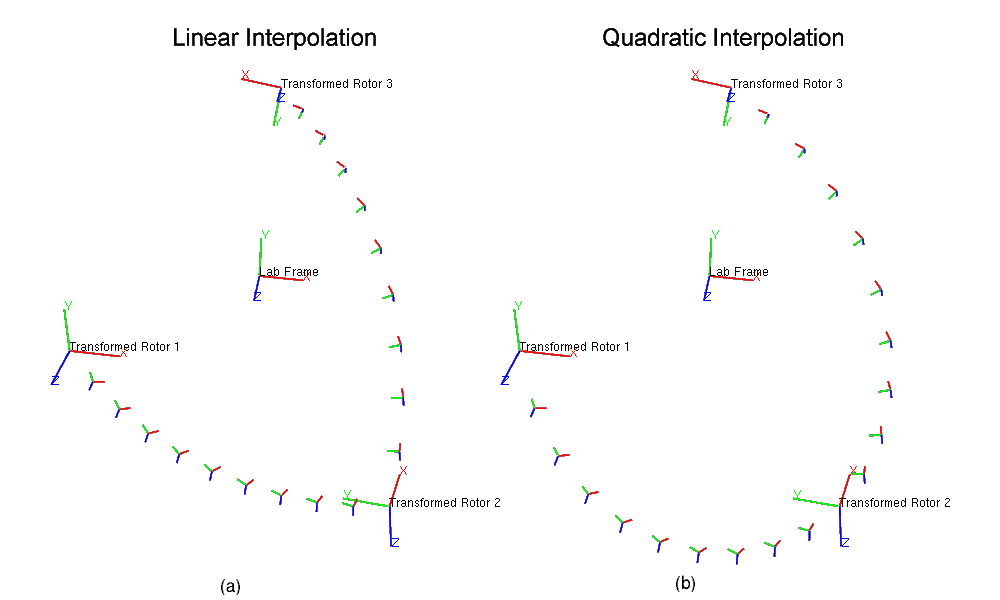
\includegraphics[width=\columnwidth]{interp}
\caption{\label{fig:interp}Examples of a) piece-wise linear and b) quadratic interpolation for
three representative poses.}
\end{figure}

\subsection{Quadratic interpolation}

Another simple form for interpolation is the quadratic interpolation where a quadratic 
is fitted through three interpolation points, $\{B_1, B_2, B_3\}$ with an interpolation
parameter varying in the range $(-1,+1)$:
\[
B'_\lambda = \left(\frac{B_3 + B_1}{2} - B_2\right)\lambda^2 + \frac{B_3 - B_1}{2}\lambda + B_2
\]
giving
\[
B'_{-1} = B_1,\quad B'_{0}=B_2\ \mbox{ and }\ B'_{+1} = B_3
\]
This interpolation varies smoothly through $B_2$ and is reflected in the final
interpolation, as shown in figure \ref{fig:interp}. Extensions to the quadratic
interpolation for more than three interpolation points, such as smoothed
quadratic interpolation \cite{cendes} are readily available.

\subsection{Alternate methods}

It is worth noting that each of the methods described above may be performed
using either direct interpolation of the bivector $\ell(R)$ corresponding
to a rotor $R$ or by interpolating the relative rotors which take one frame
to another. It is not yet clear which will give the best results and indeed
it is probably application dependent.

\section{Form of the Interpolation}

In this section we derive a clearer picture of the precise form of
a simple linear interpolation between two frames in order to relate the 
interpolation to existing methods used in mechanics and robotics. We will consider
the method used above whereby the rotor being interpolated takes one pose to another.

\subsection{Interpolation of dilations}

In certain circumstances it is desirable to add in the ability to interpolate
dilations. This was investigated in \cite{jic23fyr} and is included here
for completeness. In \cite{jic23fyr} it is shown that this can be done by extending
the form of the bivector, $B$, which we exponentiate, as follows
\[
B = \phi P + tn + \omega N
\]
where $N = e\bar{e}$. This bivector form is now sufficiently general
\cite{jic23fyr} to be able to represent dilations as well. In this case obtaining the
exponentiation
and logarithm function is somewhat involved \cite{jic23fyr}. We obtain
finally that

\[
\begin{array}{rl}
\multicolumn{2}{l}{\exp(\phi P + tn + \omega N)}\\
%\quad = & \sin(\phi)\cosh(\omega)P + \cos(\phi)\sinh(\omega)N + \cos(\phi)\cosh(\omega)+\sin(\phi)\sinh(\omega)PN \\
%&+ \frac{\omega\cos (\phi)\sinh (\omega) + \phi \sin(\phi)\cosh(\omega)}{\omega^2 + \phi^2}t_\parallel n\\
%&+ \cos(\phi)\sinhc(\omega)t_\perp n \\
%&- \frac{\omega\sin(\phi)\cosh(\omega)-\phi\cos(\phi)\sinh(\omega)}{\omega^2 + \phi^2} Pt_\parallel n \\
%&+ \sin(\phi)\sinhc(\omega)Pt_\perp n\\
\quad = & \left(\cos(\phi) + \sin(\phi)P\right)\left(\cosh(\omega) +
		\sinh(\omega)N + \sinhc(\omega)t_\Jperp n\right)\\
&+ (\omega^2 + \phi^2)^{-1} [-\omega\sin(\phi)\cosh(\omega)+\phi\cos(\phi)\sinh(\omega)]P\\
&+ (\omega^2 + \phi^2)^{-1} [\omega\cos (\phi)\sinh (\omega) + \phi \sin(\phi)\cosh(\omega)] t_\parallel n \\
	\end{array}
\]
where $\sinhc(\omega) = \omega^{-1}\sinh(\omega)$. Note that this expression reduces to 
the original form for $\exp(B)$ when $\omega = 0$, as one would expect.

It is relatively easy to use the above expansion to derive a logarithm-like inverse 
function. 

If we let $R = \exp(B)$ then we may recreate $B$ from $R$ using the method 
presented
below. Here we use $\left<R|e_i\right>$ to represent the component of $R$
parallel to $e_i$, i.e.\ $\left<R|N\right> = \left<R|e_{45}\right>$ in 
3-dimensions. We also use $\left<R\right>_i$ to represent the 
$i$-th grade-part of $R$ and $S(X)$ to represent the 
`spatial' portion of $X$ (i.e.\ those components not parallel to $e$ and 
$\bar{e}$).

\begin{tabular}{ll}
$\begin{array}{rcl}
  \omega &=& \tanh^{-1}\left(\frac{\left<R|N\right>}{\left<R|1\right>}\right)\\
  \phi &=& \cos^{-1}\left(\frac{\left<R|N\right>}{\sinh(\omega)}\right)\\
  P &=& \frac{S(\left<R\right>_2)}{\sin(\phi)\cosh(\omega)}\\
  t_\perp &=& -\frac{\left<R\right>_4-\sin(\phi)\sinh(\omega)PN}{\sin(\phi)\sinhc(\omega)}\left(\frac{P\bar{n}}2\right)\\
  t &=& t_\Jpar + t_\perp
\end{array}$ &
$\begin{array}{rcl}
  W &=& \left<R\right>_2 - \cos(\phi)\sinh(\omega)N - \sin(\phi)\cosh(\omega)P \\
  &&- \cos(\phi)\sinhc(\omega)t_\Jperp n\\
  X &=& -\omega\sin(\phi)\cosh(\omega) + \phi\cos(\phi)\sinh(\omega)\\
  Z &=&  \omega\cos(\phi)\sinh(\omega) + \phi\sin(\phi)\cosh(\omega)\\
  t_\Jpar &=& \frac{(-XP+Z)}{\sin^2(\phi)\cosh^2(\omega) + \cos^2(\phi)\sinh^2(\omega)} W
\end{array}$
\end{tabular}

\subsection{Path of the linear interpolation}

Since we have shown that $\exp(B)$ is indeed a rotor, it follows that any
Euclidean pure-translation rotor will commute with it. Thus we only need consider the
interpolant path when interpolating from the origin to some other point since
any other interpolation can be obtained by simply translating the origin to
the start point. This location independence of the interpolation is a 
desirable property in itself but also provides a powerful analysis mechanism.

\begin{figure}\centering
\includegraphics[height=1in]{plane_basis}
\caption{\label{fig:plane_basis}Orthonormal basis resolved relative to $P$.}
\end{figure}

We have identified in section \ref{subsec:form} the action of the $\exp(B)$
rotor in terms of $\psi, P, t_\parallel$ and $t_\perp$. We now investigate the resulting interpolant
path when interpolating from the origin. We shall consider the interpolant
$R_\lambda = \exp(\lambda B)$ where $\lambda$ is the interpolation co-ordinate and
varies from 0 to 1. For any values of $\psi, P, t_\parallel$ and $t_\perp$,
\[
\lambda B = \frac{\lambda \psi}{2} P + \frac{\lambda (t_\perp + t_\parallel) n}{2}
\]
from which we see that the action of $\exp(\lambda B)$ is a translation along $\lambda t_\perp$, a rotation by
$\lambda \psi$ in the plane of $P$ and finally a translation along
\[
t'_\parallel =- \sinc\left(\frac{\lambda\psi}{2}\right)
\lambda t_\parallel
\left(
\cos\left(\frac{\lambda \psi}{2}\right) -
\sin\left(\frac{\lambda \psi}{2}\right) P 
\right).
\]

We firstly resolve a three dimensional, orthonormal, basis relative to $P$ as shown in figure 
\ref{fig:plane_basis}. Here $a$ and $b$ are orthonormal vectors in the plane of $P$ and hence
$P = ab$. We may now express $t_\parallel$ as $t_\parallel = t^a a + t^b b$ where $t^{\{a,b\}}$ are suitably
valued scalars.

The initial action of $\exp(B)$ upon a frame centred at the origin is therefore to 
translate it to $\lambda t_\perp$ followed by a rotation in the plane of $P$. Due to our choice of starting
point, this has no effect on the frame's location (but will have an effect on the pose, 
see the next section).

%\begin{figure}\centering
%\includegraphics[width=0.3\columnwidth]{tan}
%\caption{\label{fig:tan} Geometric construction showing that $\beta_1 = \frac{\pi}{2} - \beta_2$.}
%\end{figure}

\begin{figure}\centering
\includegraphics[width=\columnwidth]{helix}
\caption{\label{fig:helix} Example of an interpolant path with the final location being given by
$t_\parallel = 4a + 6b$, $\psi = 9\pi$ and $t_\perp$ having a magnitude of 1.}
\end{figure}

Finally there is a translation along $t'_\parallel$ which, 
using $c = \cos\left(\frac{\lambda \psi}{2}\right)$ and $s = \sin\left(\frac{\lambda \psi}{2}\right)$,
can be expressed in terms of $a$ and $b$ as
\begin{eqnarray*}
t'_\parallel & = & - \frac{2s}{\lambda\psi} \lambda (t^a a + t^b b) (c - sab) \\
& = & -\frac{2s}{\psi} c (t^a a + t^b b) + s ( t^b a - t^a b) \\
& \equiv & -\frac{2s}{\psi} a (t^a c + t^b s) + b ( t^b c - t^a s).
\end{eqnarray*}
The position, $r_\lambda$, of the frame at $\lambda$ along the interpolation is therefore
\[
r_\lambda = -\frac{2s}{\psi} (a (t^a c + t^b s) + b ( t^b c - t^a s)) + \lambda t_\perp
\]
which can easily be transformed via the harmonic addition theorem to
\[
r_\lambda = -\frac{2s}{\psi} \alpha \left[ a \cos\left(\frac{\lambda\psi}{2} + \beta_1\right) + b \cos\left(\frac{\lambda\psi}{2} + \beta_2\right) \right] + \lambda t_\perp
\]
where $\alpha^2 = (t^a)^2 + (t^b)^2$, $\tan \beta_1 = - \frac{t^b}{t^a}$ and $\tan \beta_2 = - \frac{-t^a}{t^b}$. 
%Figure \ref{fig:tan} is a geometric construction which clearly shows by similar figures and triangle
%identities 
It is easy, via geometric construction or otherwise, to verify that this implies
that $\beta_2 = \beta_1 + \frac{\pi}{2}$. Hence $\cos(\theta + \beta_2) = - \sin(\theta + \beta_1)$. We can now express the frame's position as
\[
r_\lambda = -\frac{2\alpha}{\psi} \left[ a \sin\left(\frac{\lambda\psi}{2}\right)\cos\left(\frac{\lambda\psi}{2} + \beta_1\right) - b \sin\left(\frac{\lambda\psi}{2}\right)\sin\left(\frac{\lambda\psi}{2} + \beta_1\right) \right] + \lambda t_\perp
\]
which can be re-arranged to give
\begin{eqnarray*}
r_\lambda & = & -\frac{\alpha}{\psi} \left[ a \left(\sin\left(\lambda\psi + \beta_1\right) - \sin\beta_1\right)
+ b \left(\cos\left(\lambda\psi + \beta_1\right) - \cos\beta_1\right) \right] + \lambda t_\perp \\
& = & -\frac{\alpha}{\psi} \left[ a \sin\left(\lambda\psi + \beta_1\right)
+ b \cos\left(\lambda\psi + \beta_1\right) \right] + \frac{\alpha}{\psi} \left[
a \sin \beta_1 + b \cos \beta_1
\right] + \lambda t_\perp 
\end{eqnarray*}
noting that in the case $\psi \rightarrow 0$, the expression becomes $r_\lambda = \lambda t_\perp$ as one would
expect. Since $a$ and $b$ are defined to be orthonormal, the path is clearly some cylindrical helix with the axis of rotation passing through 
$\alpha/\psi  \left[ a \sin \beta_1 + b \cos \beta_1 \right]$.
%where the cone has an elliptical cross-section with major and minor axes aligned
%to $a$ and $b$ with magnitudes $\alpha |a|$ and $\alpha |b|$ respectively. 
An illustrative example, with $a$ and $b$ having
unit magnitude, is shown in figure \ref{fig:helix}. It also clearly shows the relation between the direction of
vector $t_\parallel$ and the final translation within the plane of $P$, $t'_\parallel$.

It is worth noting a related result in screw theory, Chasles' theorem, which
states that a general displacement may be represented using a screw motion
(cylindrical helix) such as we have derived. Screw theory is widely used in
mechanics and robotics and the fact that the na\"ive linear interpolation
generated by this method is indeed a screw motion suggests that
applications of this interpolation method may be wide-ranging, especially since
this method allows many other forms of interpolation, such as B\'ezier curves
or three-point quadratic to be performed with equal ease. Also the pure
rotation interpolation given by this method reduces exactly to the quaternionic
or Lie group interpolation result allowing this method to easily extend
existing ones based upon these interpolations.

\subsection{Pose of the linear interpolation}

The pose of the transformed frame is unaffected by pure translation and hence the initial
translation by $\lambda t_\perp$ has no effect. The rotation by $\lambda \psi$ in the plane,
however, now becomes important. The subsequent translation along $t'_\parallel$ also has
no effect on the pose. We find, therefore, that the pose change $\lambda$ along the 
interpolant is just the rotation rotor $R_{\lambda \psi, P}$.

%%%%%%%%%%%%%%%%%%%%%%%%%%%%%%%%%%%%%%%%%%%%%%%


\section{Applications}

\begin{figure}[p]
\centering
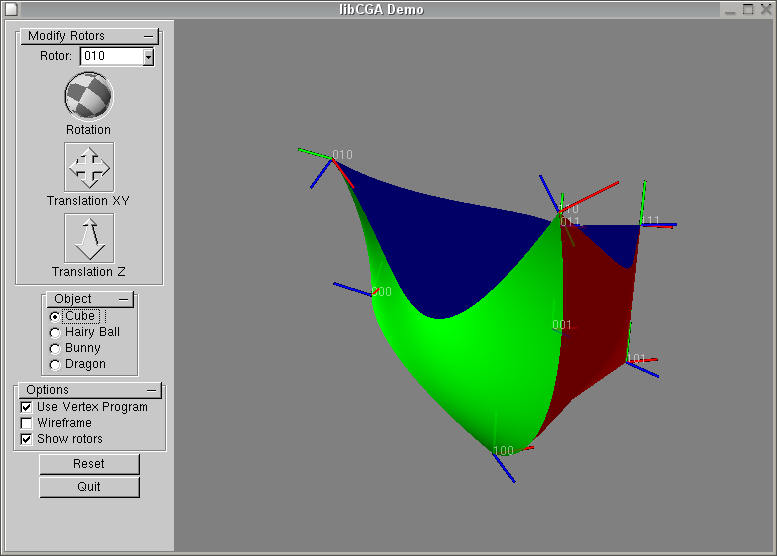
\includegraphics[width=0.7\columnwidth]{distorted_cube}
\caption{\label{fig:distorted_cube}%
  A cube distorted via the linear interpolation of rotors specifying its
  corner vertices.
}
\end{figure}

\begin{figure}[p]
\centering
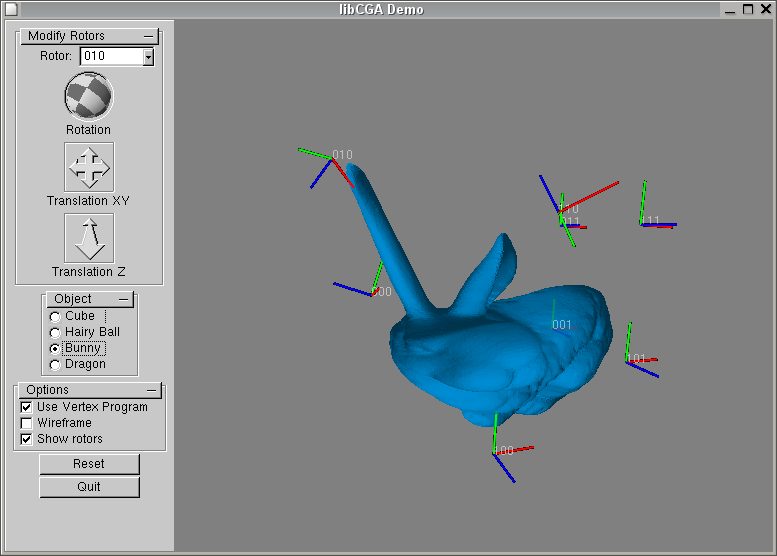
\includegraphics[width=0.7\columnwidth]{distorted_bunny}
\caption{\label{fig:distorted_bunny}%
  The Stanford Bunny\cite{bunny} distorted by the same rotors.
}
\end{figure}

The method outlined is applicable to any problem which requires the smooth
interpolation of pose. We have chosen to illustrate an application in
mesh deformation. Smooth mesh deformation is often required in medical 
imaging applications \cite{ACM:614422} or video coding \cite{ACM:704422}.
Here we use it to deform a 3d mesh in a manner which has a visual effect
similar to `grabbing' a corner of the mesh and `twisting' it into place.
We do this by specifying a set of `key-rotors' which certain parts of the
mesh must rotate and translate to co-incide with. Our implementation takes
advantage of the hardware acceleration offered by the Graphics
Processing Units (GPUs) available on today's consumer-level graphics 
hardware. A full discussion of the method will appear elsewhere.

We believe this method leads to images which are intuitively related to
the rotors specifying the deformation. Furthermore, the method need not
only be applied to meshes with simple geometry and can readily be applied to
meshes with complex geometry without any tears or other artefacts appearing
in the mesh. Figures \ref{fig:distorted_cube} and \ref{fig:distorted_bunny}
illustrate the method in the case of a cube and a mesh with approximately
36,000 vertices.



\begin{savequote}
\quoteperson{They can't keep this level of graphics up for much longer!
We used to be lucky if we only got three shades of grey, let alone any 
real colours!}{Cranky Kong}
\end{savequote}

\chapter{Hardware Assisted Geometric Algebra on the GPU}

In this chapter we explore how the \emph{Graphics Processing
Units} (GPUs) in modern consumer-level graphics cards can be
used to perform Geometric Algebra computations faster than a 
typical single-core CPU.

\section{An Overview of GPU Architecture}

\begin{figure}
\centering
\includegraphics[width=0.9\textwidth]{gpu_architecture}
\caption{\label{fig:gpu_architecture}%
  A simplified block diagram of a typical GPU.}
\end{figure}

The GPU in a graphics card is not designed for general purpose 
computing. It is designed, not surprisingly, to perform the
sort of operations useful for graphics rendering. Figure
\ref{fig:gpu_architecture} shows a simplified block diagram of
a typical GPU.

In a traditional fixed-function GPU the CPU uploads, over the AGP
bus, a set of vertices, texture maps and some state information. The
state includes projection and view matrices, clipping planes, 
lighting models, etc. The vertex list and texture maps (if present) 
are then stored in some on-card memory.

On the card there exists a number of rendering pipelines, each of which
can be run in parallel to increase throughput. The pipeline consists
of a \emph{vertex shader} which fetches triplets of vertices from
the vertex memory, transforms them using the current projection and 
view matrices, performs any clipping and sends them to the rasterizer.

The rasterizer takes triplets of screen co-ordinate vertices, forms
a triangle from them and outputs a set of pixel positions which form
render the triangle along with depth information and interpolated texture
co-ordinates. 

The fragment shader takes these pixel positions and, using the texture maps
stored in texture memory along with appropriate state information calculates
the colour of the pixel after all lighting, etc. is performed. The shaded pixel
is then sent to the screen.

In reality the rendering stage is split at the rasterizer allowing for differing
numbers of vertex and fragment shaders but for the purposes of GPU programming
one can view the shaders as being within the same pipeline.

In modern programmable GPUs both the vertex and fragment shaders are fully 
programmable allowing different per-vertex and per-pixel transformation
and shading that is allowed in the traditional fixed-function pipeline.

Each shader is, in effect, an efficient vector processor and, on modern 
graphics cards, there are a number working in parallel. To perform
general purpose computation on the GPU we must find ways of modifying our
algorithms to fit this model.

\section{GPU Programming Methods}

\subsection{DirectX shader language}

Microsoft's DirectX\cite{GPU:DirectX} is a graphics programming API for
Windows and, to some extent, the Microsoft XBox gaming platform. As part of
the API it specifies a generic shading language\cite{GPU:DirectXShadingLanguage}
which abstracts the vertex and fragment shaders. Each version of DirectX
specifies a minimum set shader capabilities which \emph{must} be supported by a 
card claiming compatibility with that level of the API. Consequently a shader written in
DirectX's shading language is portable across all cards which support that level
of the API. A disadvantage of DirectX is that it doesn't expose any functionality
beyond the specified minimum and it is not portable across operating systems.

\subsection{OpenGL shader language}

OpenGL\cite{GPU:OpenGLSpec} is a cross-platform C-based graphics API. 
It is the \emph{de facto} standard API for non-Windows platforms and
is well supported on Windows platforms by both ATI and nVidia, the dominant
vendor at the time of writing. 

The OpenGL 2.0 specification\cite{GPU:OpenGL2Overview} proposed by 3DLabs
includes a hardware agnostic shading language\cite{GPU:OpenGLShadingLanguage}
known as \emph{GL Shading Language} (GLSL) which provides a similar level
of functionality to that exposed in DirectX. 

Currently few hardware vendors support OpenGL 2.0 --- at the time of writing
nVidia was the only mainstream vendor to provide support in their
consumer-level hardware\cite{nvidia:7664relnotes}.

OpenGL 1.4 and below provide support for programmable shaders via a set of per-vendor
extensions. Unfortunately these requires programming the GPU in a variety of
assembly languages and vary between different GPUs.

\subsection{The Cg toolkit from nVidia}

Both the OpenGL and DirectX shading languages have a number of disadvantages
from the point of view of research. The OpenGL shading language, whilst being
high-level and convenient to program in, is not widely available. The
DirectX toolkit provides only a `lowest common denominator' shading language,
it is not particularly high-level and is, for all intents and purposes, limited
to the Microsoft Windows operating systems. 

An attempt to bridge these gaps is the Cg toolkit\cite{nvidia:cgtoolkit} from nVidia.
It provides a high-level C-like shading language which may be compiled at run-time or
ahead of time into either DirectX shading language or the myriad of OpenGL extensions
which exist for accessing the programmable shaders. 

Along with these advantages is the `future-proof' nature of Cg. The core Cg language
is easily extended via so-called `profiles'. These either restrict the language to
correspond to the capabilities of particular GPUs or add more features to expose
new GPU abilities. As an example in figure \ref{fig:gpu_architecture} it was implied
that the vertex shader cannot access the texture-map memory. This was true
of older cards but the latest generation of nVidia cards can
access texture maps from within the vertex shader\cite{nvidia:sm3unleashed}. Adding this
capability to Cg was simply a case of releasing a new profile where texture-map related
parts of the language were now available from within both shaders. Older shaders
would still work however and the presence of this capability could be queried
at run-time.

Because of these advantages it was decided to use Cg as the basis for the GPU
computing research. None of the techniques described below require it as they
can all be re-structured to use alternate APIs.

\section{A Cg Implementation of Generator Exponentiation}

\begin{figure}[p]
\centering
\scalebox{0.8}{
\begin{minipage}{0.8\textwidth}
\singlespacing
\lstinputlisting[language=c]{rotor_tools.cg}
\hrule
\lstinputlisting[language=c]{rotor_tools.h}
\end{minipage}}
\caption{\label{fig:rotortools}The Cg and C interfaces for dealing with rotors and
  exponentiated generators.}
\end{figure}

In order to integrate the GA interpolation scheme described in the previous 
chapter into the GPU graphics pipeline it had to be re-cast into the 
mathematical language of the GPU. Graphics cards are optimised for 
linear algebra on 4-dimensional vectors and $4\times4$ matrices, reflecting
the dominant language used in graphics. 

It was decided to abstract away the GA method and represent rotors and
generators as sets of vectors. The Cg interface, and corresponding CPU-side C
interface, used is shown in figure \ref{fig:rotortools}. The required GA
operations for rotor exponentiation and application ($X \mapsto RX\tilde{R}$)
were expanded out in terms of basis components and implemented
directly in Cg. The routines could now be used as a `black-box' by the GPU 
programmer. Indeed no GA knowledge was required for their use, merely that one
applies rotors to points to transform them, one can convert generators into
rotors and generators may be linearly interpolated.

A more general GA-solution, such as {\tt libcga}, was impractical given the
current space constraints on Cg programs although future GPUs may provide
enough space to make such a library feasible.

\section{Mesh Deformation}

In this section we shall give an example of a vertex shader that uses GA to
perform mesh deformation. The deformation scheme given is a simple application
of Geometric Algebra to the problem but nicely shows the applicability of GA
to a wide variety of problems. The method developed has a number of nice 
properties but should be viewed as an illustration of the power of GA
algorithms when implemented on the GPU rather than as a deformation scheme
in its own right.

\subsection{Method}

We shall now present a GA-based mesh deformation scheme suitable for
implementation on a GPU. In this scheme we start with
an existing mesh and set of key rotors, $\left\{ R_1, R_2, \cdots, R_k \right\}$,
which we wish to use to deform the mesh. Our scheme seeks to find some automatic
method of representing each point on the mesh as some function of the key
rotors; changing the key rotors will then lead to a deformation of the mesh. Desirable
properties include smoothness, small changes in the rotors lead to small changes
in the mesh, and to be intuitive, changes in the rotors should produce changes
in the mesh which a user, ignorant of the method, would expect.

\begin{figure}
\centering
\includegraphics[width=0.8\textwidth]{assignment_scheme}
\caption{\label{fig:assignment_scheme}Representing a point, $P_i$, on a mesh as
a rotor, $R_i$, and displacement, $p_i$, given a set of key rotors, 
  $\left\{R_1, R_2\right\}$.}
\end{figure}

Our assignment scheme is illustrated in figure \ref{fig:assignment_scheme}.
Firstly we form a set of generators, $\left\{B_1, B_2, \cdots, B_k\right\}$,
such that
\[
\left\{ R_1, R_2, \cdots, R_k \right\} \equiv \left\{\exp(B_1), \exp(B_2),
        \cdots, \exp(B_k)\right\}.
\]
We also find the image of the origin, $O_k = R_k\bar{n}\tilde{R}_k$, for 
each key-rotor. For each point-representation on the mesh, $P_i$, we find the Euclidean
distance from it to the image of the origin in each key-rotor,
\[
\label{eqn:dki}
d_{k,i} = \sqrt{-2O_k \cdot P_i}.
\]
We then form a rotor, $R_i$, for each point on the mesh as a weighted sum of the
key-rotors,
\[
R_i = \exp\left(\frac{\sum^{k}_1 w_i(d_{k,i}) B_i}{\sum^{k}_1 w_i(d_{k,i})}\right)
\]
where $w_i(d)$ is a function which defines the relative weights of each rotor depending
on its proximity to the mesh point. One might choose a relatively simple weight function
\[
w_i(d) = \frac{1}{d + \epsilon}
\]
where $\epsilon$ is a small value to avoid a singularity when the key-rotor and mesh
intersect. In our implementation we wished to have key-rotors with varying degrees of 
influence. This was accomplished by using a Gaussian weight function,
\[
w_i(d) = \exp\left(-\frac{d^2}{\sigma_i^2}\right)
\]
with $\sigma_i$ giving the radius of influence of a particular key-rotor.

Finally we find a point, $p_i$, which is transformed by $R_i$ to coincide
with $P_i$,
\[
(R_i p_i \tilde{R}_i) \cdot P_i = 0
\]
which may be found by simply applying the reversal of $R_i$ to $P_i$
\[
p_i = \tilde{R}_i P_i R_i.
\]
The point $P_i$ is now stored in memory as a set of $d_{k,i}$ for each
key-rotor and the point $p_i$.

Our deformation procedure is now simple. Given a new set of key-rotors,
$\left\{ R'_1, R'_2, \cdots, R'_k \right\}$, and a corresponding set of
generators, $\left\{B'_1, B'_2, \cdots, B'_k\right\}$, we can form the deformed
mesh point $P'_i$ given the previously calculated $d_{k,i}$ and $p_i$ as
\begin{align}
R'_i &= 
\exp\left(\frac{\sum^{k}_1 w_i(d_{k,i}) B'_i}{\sum^{k}_1 w_i(d_{k,i})}\right) \label{eqn:summation} \\
P'_i &= R'_i p_i \tilde{R}'_i.
\end{align}
It is easy to show by direct substitution that for $R'_k = R_k$ this 
reduces to $P'_i = P_i$ as would be expected.

\subsection{GPU-based implementation}

Since the GPU distinguishes between global state and per-vertex information we
must decide what information needs to be given to the GPU and how. In our mesh
deformation example we need the key-rotors which are part of the global state
and, for each mesh point, the vector $p_i$ and set of distances $d_{k,i}$.

In OpenGL each vertex has at least a three-dimensional position vector associated 
with it and may have a normal vector. In addition there are a number of 
texture co-ordinates which may be associated with each vertex. In our implementation
the values of $w(d_{k,i})$ will be stored into the texture co-ordinates. The weight
function is pre-computed to save time.

\begin{figure}[p]
\centering
\scalebox{0.8}{
\begin{minipage}{\textwidth}
\singlespacing
\lstinputlisting[language=c]{vertex_shader.cg}
\end{minipage}}
\caption{\label{fig:meshshader}The vertex shader used to perform GA-based mesh
deformation.}
\end{figure}

Figure \ref{fig:meshshader} gives the vertex shader used to perform mesh deformation in
this example. Line 2 includes the standard set of rotor manipulation functions which
were described above. 
%For the moment it is sufficient to note that generators are
%stored as a pair of 3-vectors, giving 6 components in all, and rotors are stored as a
%pair of 4-vectors, giving 8 components.

The generators associated with the key rotors are passed in the state array {\tt generators[][]}
and are constant for a particular scene. Lines 32 to 39 perform the summation in 
equation \ref{eqn:summation} and line 41 uses the function {\tt exp\_generator()} to 
form $R'_i$. Line 42 applies $R'_i$ to the point $p_i$ and the remainder of the shader
is boilerplate code to project into screen-space and perform a simple lighting calculation.

\begin{fancyalg}
\begin{algorithmic}[1]
\REQUIRE{$P_i$, the null-vector representation of mesh vertex $i$.}
\REQUIRE{$\mathcal{B} \equiv \{B_1, B_2, \cdots, B_k, \cdots \}$,
  the set of key-rotor generators.}
\STATE $w_{\mathrm{sum}} := 0$
\FOR{$k := 1$ to $n(\mathcal{B})$}
\STATE $R := \exp(B_k)$
\STATE $O := R\bar{n}\tilde{R}$
\STATE $w_k := w(\sqrt{-2 O \cdot P})$
\STATE $w_{\mathrm{sum}} := w_{\mathrm{sum}} + w_k$
\ENDFOR
\FOR{$k := 1$ to $n(\mathcal{B})$}
\STATE $w_k := \frac{w_k}{w_{\mathrm{sum}}}$
\ENDFOR
\STATE $p := \tilde{R}P_iR$
\STATE glMultiTexCoord2f(GL\_TEXTURE0, $w_1$, $w_2$);
\STATE glMultiTexCoord2f(GL\_TEXTURE1, $w_3$, $w_4$); 
\STATE glMultiTexCoord2f(GL\_TEXTURE2, $w_5$, $w_6$);
\STATE glMultiTexCoord2f(GL\_TEXTURE3, $w_7$, $w_8$);
\STATE glVertex($p$);
\end{algorithmic}
\caption{\label{alg:meshpoint}Algorithm for computing $w(d_{k,i})$ and $p_i$ for 
  each mesh point and storing them in the texture co-ordinates and vertex position.
  In this case there are eight key-rotors.}
\end{fancyalg}

The algorithm and OpenGL code required to compute the rotor weights and offset-vector
$p_i$ for each mesh vertex is shown in algorithm \ref{alg:meshpoint}. Note that this
need only be performed once-per vertex at initialisation.

In the actual implementation \emph{display lists} were utilised. A display list 
is an OpenGL technique for uploading a set of OpenGL calls to the graphics card
and executing them again with one call. Since the vertices and texture co-ordinates
generated by algorithm \ref{alg:meshpoint} don't change once calculated each mesh could
be processed once and sent to the graphics card as a display list.

Using a display list meant that the deformation now became extremely efficient in
terms of CPU usage. For each frame all that needed to be done by the CPU was update the
state variables holding the key-rotor generators and ask for the display list to be drawn.
Using such a technique resulted in the Unix \emph{top} utility reporting 0\% CPU utilisation,
i.e. below the resolution it measures to.

\subsection{Quality of the deformation}

\begin{figure}[p]
\centering
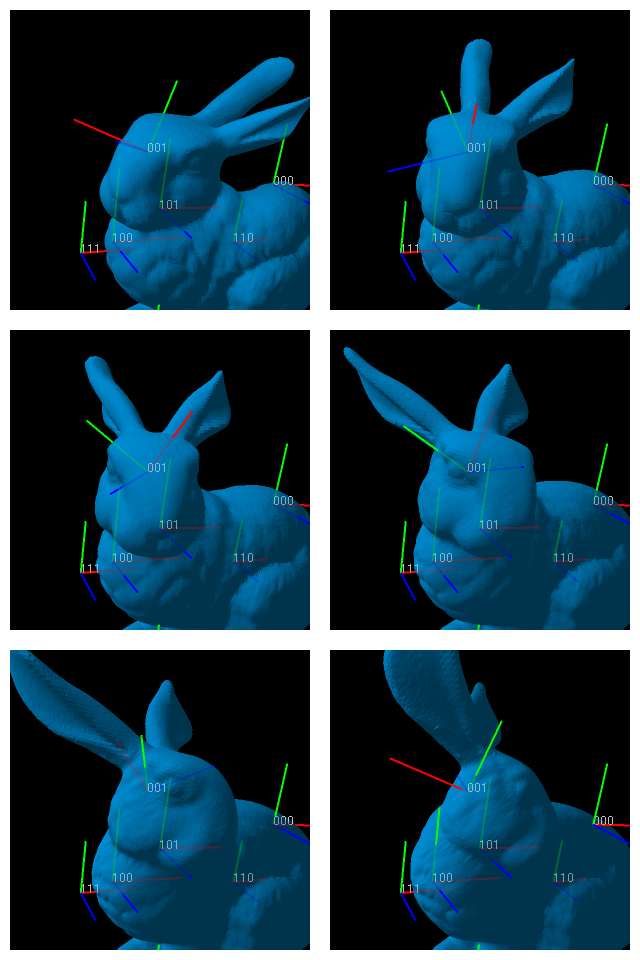
\includegraphics[height=0.8\textheight]{mesh_example}
\caption{\label{fig:meshexample}An example of animating a rabbit's head using key-rotors and an automatically
  assigned mesh.}
\end{figure}

The quality of a mesh deformation technique is ultimately subjective. A simple
example is shown in figure \ref{fig:meshexample}. In this example there were
eight key rotors labelled `000' to `111' in binary. The rotors were moved to
positions within a rabbit model and appropriate weighting and offset-vectors
were assigned using algorithm \ref{alg:meshpoint}. The `001' rotor, which was
positioned within the rabbit's head, was then moved and the results are shown.
The movement is smooth, natural and intuitive.

\begin{figure}[p]
\centering
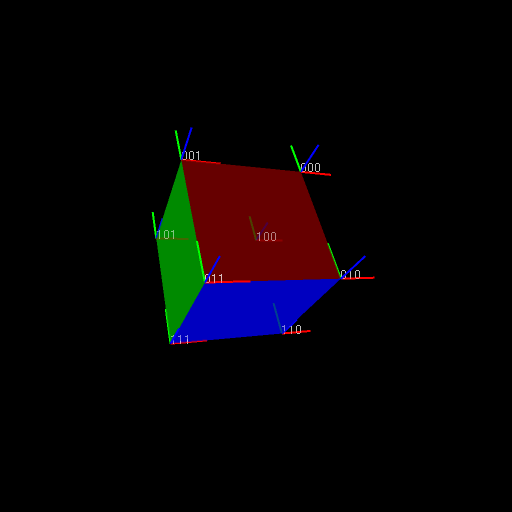
\includegraphics[height=0.37\textheight]{cube_before} \\
\noindent (a) \\ \rule{0pt}{\parskip} \\
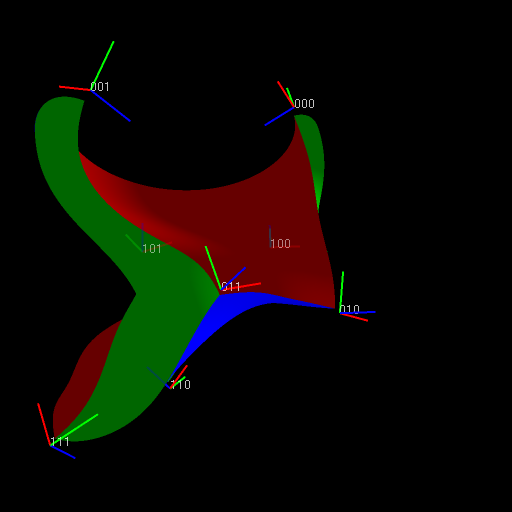
\includegraphics[height=0.37\textheight]{cube_after} \\
\noindent (b) 
\caption{\label{fig:cubeexample}An example of mesh deformation acting on a unit cube.
  (a) Initial key-rotors and automatically assigned mesh. 
  (b) Deformed mesh after movement of key-rotors.} 
\end{figure}

\begin{figure}[p]
\centering
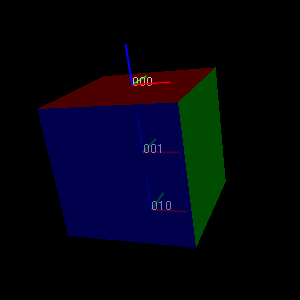
\includegraphics[height=0.37\textheight]{twist_cube_before} \\
\noindent (a) \\ \rule{0pt}{\parskip} \\
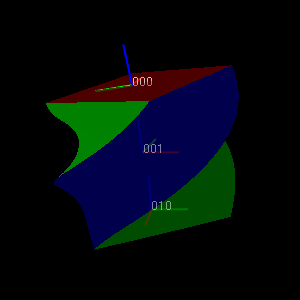
\includegraphics[height=0.37\textheight]{twist_cube_after} \\
\noindent (b) 
\caption{\label{fig:twistcubeexample}An example of twist deformation acting on a unit cube.
  (a) Initial key-rotors and automatically assigned mesh. 
  (b) Twisted mesh after movement of key-rotors.} 
\end{figure}

Figure \ref{fig:cubeexample} shows the natural `plasticine-like' effect the deformation
scheme has on a unit cube with key-rotors initially placed on it's corners. In addition to
this figure \ref{fig:twistcubeexample} shows the effect of placing the key rotors along
a central axis and applying opposite rotations at either end. Notice how the cube behaves as
expected and does not collapse in the middle.

\subsection{Performance}

\begin{table}[p]
\centering
\scalebox{0.8}{%
\begin{tabular}{|c|c|c|c|}
\hline                 
 & \multicolumn{2}{c|}{Frames per second} & \\
\hline                 
Polygons & Hardware & Software & Ratio \\
\hline                 
\hline                 
14,406 & 219.10 & 18.81 & 11.65:1\\
20,886 & 160.80 & 12.50 & 12.86:1\\
29,400 & 119.50 & 9.08 & 13.16:1\\       
43,350 & 83.91 & 6.26 & 13.40:1\\
60,000 & 62.13 & 4.65 & 13.36:1\\
\hline                 
\end{tabular}%
\hspace{3ex}
\begin{tabular}{|c|c|c|c|}
\hline                 
 & \multicolumn{2}{c|}{Frames per second} & \\
\hline                 
Polygons & Hardware & Software & Ratio \\
\hline                 
\hline                 
93,750 & 20.42 & 2.89 & 7.07:1\\        
135,000 & 14.20 & 2.07 & 6.86:1\\
240,000 & 8.13 & 1.14 & 7.13:1\\         
372,006 & 5.32 & 0.75 & 7.09:1\\         
-- & -- & -- & -- \\
\hline                 
\end{tabular}
}
\caption{\label{tab:performance}The relative performance, in frames per
second, between the GPU and pure-software mesh deformation implementations.%
}
\end{table}

\begin{figure}[p]
\centering
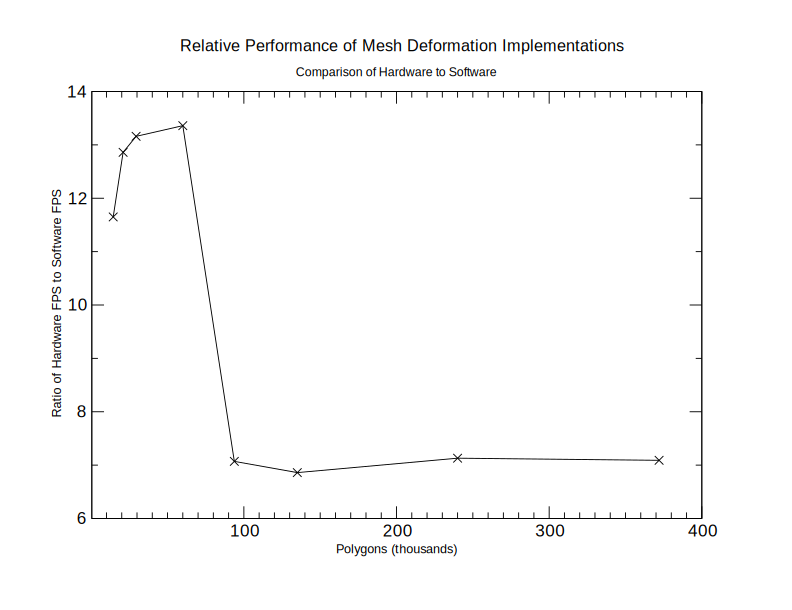
\includegraphics[width=0.9\textwidth]{performance}
\caption{\label{fig:performance}A plot of the ratio between FPS using the
GPU-based implementation and the pure-software implementation.}
\end{figure}

To test the relative performance of software and hardware two implementations
were made, one software and one hardware. Both implemented the same mesh deformation
algorithm as above and both used as near equal, within the intersection of C and
Cg, implementations of the generator exponentiation and rotor application
routines.

The implementations differed most in the use of display lists. To mirror real-world
practises each model in the hardware implementation was uploaded to the graphics
card in a display list since the per-vertex set of $d_{k,i}$ and $p_i$ could
be pre-computed. In the software implementation these were also pre-computed but the
deformed vertices had to be uploaded to the graphics card once-per frame since the
deformation step was done in software.

Table \ref{tab:performance} shows the number of frames per second that could be
displayed with a simple cube model at various different polygon count. A simple model
was chosen so that the generation, per frame, of un-deformed model vertices in the
software implementation would take as little time as possible being 
algorithmically generated rather than fetched from main memory providing a fairer
test of the speeds of the deformation algorithm. Figure \ref{fig:performance} shows
the ratio of improvement between software and hardware implementations with polygon
count.

\section{Dynamics}

In this section we will develop a simple method for doing dynamics with a sphere
which has been deformed with a set of rotors. We shall show how a simple dynamics example
using such a method may be implemented on the GPU.

Recall that a GPU has two classes of shaders; it has vertex shaders which are applied
per-vertex and fragment shaders which are applied per-pixel. Since, in a typical scene,
one would expect the number of pixels on screen to be very much greater than the number
of vertices, GPUs generally have more parallel fragment shaders than vertex shaders.
If we can re-formulate our solution to use fragment shaders we might expect even
greater performance than simply using the vertex shader.

Algorithms implemented on the fragment shaders have one further 
advantage when compared to those implemented on the vertex shader when one makes use
of the \emph{render to texture} feature on modern graphics cards. Using this feature
rendering can be directed to a texture stored in the graphics card memory rather than the
screen. This feature allows iterative algorithms to be developed.
The concept is simple. A texture is created which stores a set of initial values. 
A square is then rendered with a fragment shader which, for each pixel in the square,
reads the initial value from the texture and outputs the result of the next iteration.
If this square is rendered into the original texture then the result of each iteration
replaces the previous one. This process may be repeated as often as is desired.
In reality there are a few implementation issues. Aside from the API calls required to
setup the render to texture and appropriate projection matrices a significan issue is
that the shader is required to write back to its input which could lead to
concurrency issues. To avoid this one generally uses two textures, an `input' and `output',
which are swapped between each iteration.

\subsection{Collision detection via deformation}

\begin{figure}
\centering
\includegraphics[width=0.8\textwidth]{deformation_scheme}
\caption{\label{fig:deformation_scheme}Given a deformation scheme $\mathcal{D}$ which maps
  our object to the unit sphere we can tell whether a point, $P$, is inside the object by
          testing if the mapped point, $P'$, is inside the sphere.}
\end{figure}

We shall develop a simple example to illustrate this method. In our example we
shall implement an approximate simulation of a cloth falling onto a complex
smooth object. 

To begin with we need a GPU-based simulation of the cloth itself for when
it is moving in space away from the target object. The aim of this example is
to demonstrate complex collision rather than cloth simulation \emph{per se}
and so we choose a very simple ball and spring model; the cloth is composed
of a $N\times M$ grid of masses connected by simple Hookian springs. Formally, 
if we let $P_{i,j}$
be the position vector of the ball in row $i$, column $j$ then the force acting
on it, $F_{i,j}$ is
\[
F_{i,j} = \sum_{\alpha \in \{-1,1\}} \sum_{\beta \in \{-1,1\}} 
b_{i+\alpha, j+\beta} 
\left| P_{i,j} - P_{i+\alpha, j+\beta} \right|
\]
where
\[
\left\{
b_{i,j} = \begin{array}{ll}
1 & {\rm ~if~} i \in \{1, \cdots, N\}, j \in \{1, \cdots, M\} \\
0 & {\rm ~otherwise}
\end{array}
\right.
\]
The variation of $P_{i,j}$ over time may then be obtained by numerically
integrating the force twice.

Such simple dynamics are often employed in games where the appearance of
correct physics is often more desireable, if it is faster, than a full
`correct' calculation. We shall use a common game technique[FIXME:reference]
which may be summarised as `detect and backtrack'.

Suppose a cloth vertex were to be outside of the target object at time
$t$ and we detect it is to be inside the object at time $t + \Delta t$. 
We stop the simulation and backtrack to time $t + \Delta t - t_{\rm offset}$
with $t_{\rm offset} < \Delta t$ such that the vertex is just touching
the target object. We then use simple surface physics to modify the total
force acting on the vertex to cause reflection, friction or any other 
surface property we may wish. The simplation is then restarted from this point.

We shall discuss the precise implementation of the cloth simulation later but
for the moment we note that the key operation is detecting the interpenetration
of the grid of cloth vertices and the target object,

Our approach is illustrated in figure
\ref{fig:deformation_scheme}. We shall assume some GA-based deformation scheme
$\mathcal{D}$ which will deform our target object to the unit sphere.
%Ideally this
%deformation scheme should preserve both position and orientation information
%so that we can perform physics on the unit sphere and deform the result back
%to our original object.
If we apply the same deformation scheme to the current cloth state the
interpenetration test for each cloth vertex is simply to test if its distance
from the origin is less than unity. If so, we can correct by simply moving
the point to the unit-sphere surface and revert the deformation to obtain the
new cloth collision

\subsection{Cloth dynamics}



\begin{figure}[p]
\centering
\scalebox{0.7}{
\begin{minipage}{\textwidth}
\singlespacing
\lstinputlisting[language=c]{map.cg}
\end{minipage}}
\caption{\label{fig:map}The vertex shader utility functions for mapping to and
  from a rotor-deformed space.}
\end{figure}




\chapter{Conclusions and Future Work}

In this chapter we shall collate all of the findings from the previous chapters
and give them a context in relation to each other. Future applications for
the various findings will be discussed.

\section{Review of Achievements}

In this section we briefly review the achievements and findings from each
chapter.

\subsection{Non-Euclidean geometries}

In chapter \ref{chap:noneuclid} a framework for extending the conformal
model to deal with non-Euclidean geometries was developed with particular
emphasis on hyperbolic geometry. It was shown that the geometry
represented by a model is entirely determined by the choice of null-vector
representation and rotors. The pure-rotation and pure-translation 
rotors for hyperbolic space were derived and it was shown that the usual
distance metric for hyperbolic geometry could be obtained therefrom.

Already some work using the conformal model to represent non-Euclidean geometry
has found application in cosmology\cite{GA:SIGKEY} has been done leading, potentially, to important insights on
our Universe.

\subsection{Fractals}

In chapter \ref{chap:fractals} an extension to complex numbers, similar to that
of quaternions, was developed for arbitrary dimension. It was noted that, in
GA, quaternions are simply special cases of a wider variety of algebras. This
extension was used to form a dimension-agnostic formulation for the classic
complex iteration-based Julia and Mandelbrot fractal sets. In addition an
existing distance estimation formula was shown to be valid using this extension
allowing for the ray-tracing of arbitrary dimension sets.

Real-world applications of fractals are notoriously difficult to find but the
opening up of escape-time fractals to non-Euclidean geometries provides a
number of opportunities for `recreational mathematics' and the generation of
attractive images.

\subsection{Rotor exponentiation}

In chapter \ref{chap:exponential} it was hypothesised that all the rotors we
used in the conformal model could be obtained by exponentiating a corresponding
generator bivector the components of which would be geometrically meaningful.
A closed form solution for \emph{both} the exponentiation and subsequent
inverse exponentiation (modulo the identification of rotations by $2n\pi$) was
derived.

From this an algorithm for directly mapping the components of the generator
to a $4 \times 4$ matrix suitable for use in existing graphical pipelines
was developed. A matching algorithm for directly converting a matrix to
a generator, again identifying rotations of $2n\pi$, was also developed.

This particular chapter has almost limitless application. Not only is the
linear space of the bivectors mapped to the non-linear space of rigid-body
transformations but the appropriate inverse mapping was also defined. Using
this method many existing linear optimisation algorithms or interpolation
schemes could be extended to deal with rotation and translation
\emph{simultaneously}.

\subsection{GPU-based techniques}

In chapter \ref{chap:gpu} the techniques developed in chapter \ref{chap:exponential}
were implemented on the programmable portion of modern Graphics Processing
Units. Such \emph{shaders} were used to develop sample graphics algorithms which
made use of the mappings developed in this thesis. 

Specifically simple mesh deformation and collision detection examples were show.
The examples demonstrated that not only was GA a natural language for developing
such algorithms allowing one to use much geometric insight but they were also
compact enough to program so that they could be efficiently implemented in hardware.

\section{Future work}



\end{mainmatter}

% \nocite{*}

\begin{backmatter}
\bibliography{geometry,ga,fractals}
\end{backmatter}

\end{document}
